\Opensolutionfile{ans}[ans/ansCD2D3-3.1.1]
\section{ỨNG DỤNG CỦA TÍCH PHÂN}
\subsection{Kiến thức sách giáo khoa cần cần nắm}
\subsubsection{DIỆN TÍCH HÌNH PHẲNG}
\textbf{1. Định lý 1: }Cho hàm số $y=f(x)$ liên tục, không âm trên $[a;b]$. Khi đó diện tích $S$ của hình thang cong giới hạn bởi đồ thị hàm số $y=f(x)$, trục hoành và 2 đường thẳng $x=a,x=b$ là $S=\displaystyle\int\limits_a^b f(x)\mathrm{\,d}x$.\\
\textbf{2. Bài toán liên quan.}\\
\textbf{\textit{Bài toán 1: }}Diện tích hình phẳng giới hạn bởi đồ thị hàm số $y=f(x)$ liên tục trên đoạn $[a;b]$, trục hoành và hai đường thẳng $x=a$, $x=b$ được xác định: $S=\displaystyle\int\limits_a^b|f(x)|\mathrm{\,d}x.$ 
\begin{center}
	\begin{tikzpicture} [scale=1,yscale=.7, font=\footnotesize, line join=round, line cap=round, >=stealth]
	\def \xmin{-1} \def \xmax{5.5}
	\def \ymin{-1.3} \def \ymax{3.2} 
	\draw[-stealth] (\xmin,0)--(\xmax,0) node [below]{$x$};
	\draw[-stealth] (0,\ymin)--(0,\ymax) node[left]{$y$};
	\path (0,0) circle(1pt) node[below left]{$O$};
	\draw [] (0,0.2)-|(0.2,0);
	\def \f(#1){0.2*((#1)-.5)*((#1)-2)*((#1)-3)*((#1)-4.2)*((#1)-5.2)}
	\pgfmathsetmacro \fa{\f(1)}
	\pgfmathsetmacro \fb{\f(4.85)}
	\begin{scope}
	\clip (\xmin,\ymin) rectangle (\xmax,\ymax); 
	\fill[pattern=north west lines,opacity=10] plot[domain=1:4.85](\x,{\f(\x)})--plot[domain=4.85:1](\x,{0});
	\end{scope}
	\draw[samples=200,smooth,domain=1:4.85] plot (\x,{\f(\x)});
	\draw (1,0)--(1,\fa) (4.85,0)--(4.85,\fb);
	\foreach \x/\g in {1/a,2/c_1,3/c_2,4.2/c_3} 
	\draw[fill] (\x,0) circle(1pt)+(-90:4mm) node {$\g$} ;
	\path (3.5,1) node {$y=f(x)$} (4.85,0) node[below right] {$b$};
	\end{tikzpicture}
\end{center}
\textbf{\textit{Bài toán 2: }}Diện tích hình phẳng giới hạn bởi đồ thị hàm số $y=f(x)$, $y=g(x)$ liên tục trên đoạn $[a;b]$ và hai đường thẳng $x=a$, $x=b$ được xác định: $S=\displaystyle\int\limits_a^b|f(x)-g(x)|\mathrm{\,d}x.$ 
\begin{center}
	\begin{tikzpicture} [scale=1,yscale=.7, font=\footnotesize, line join=round, line cap=round, >=stealth]
	\def \xmin{-1} \def \xmax{5.5}
	\def \ymin{-1.3} \def \ymax{5.5} 
	\draw[-stealth] (\xmin,0)--(\xmax,0) node [below]{$x$};
	\draw[-stealth] (0,\ymin)--(0,\ymax) node[left]{$y$};
	\path (0,0) circle(1pt) node[below left]{$O$};
	\draw [] (0,0.2)-|(0.2,0);
	\def \f(#1){((#1)-.2)*((#1)-2)*((#1)-3)}
	\def \g(#1){((#1)-1.2)*((#1)-2)}
	\pgfmathsetmacro \ga{\g(.3)}
	\pgfmathsetmacro \fa{\f(.3)}
	\pgfmathsetmacro \fb{\f(3.75)}
	\begin{scope}
	\clip (\xmin,\ymin) rectangle (\xmax,\ymax); 
	\fill[pattern=north west lines,opacity=10] plot[domain=.3:3.73](\x,{\f(\x)})--plot[domain=3.73:.3](\x,{\g(\x)});
	\end{scope}
	\draw[samples=200,smooth,domain=.3:3.85] plot (\x,{\f(\x)});
	\draw[samples=200,smooth,domain=.3:3.85] plot (\x,{\g(\x)});
	\draw[dashed] (.3,0)--(.3,\ga) (3.73,0)--(3.73,\fb) ;
	\draw (.3,\ga)--(.3,\fa);
	\foreach \x/\g in {.3/a,1.2/c_1,2/c_2,3.73/b} 
	\draw[fill] (\x,0) circle(1pt)+(-90:4mm) node {$\g$} ;
	\path
	(1,2) node {$y=f(x)$}
	(1.3,-.9) node {$y=g(x)$}
	;
	\end{tikzpicture}
\end{center}
\textbf{Chú ý:}\\
- Nếu trên đoạn $[a;b]$, hàm số $f(x)$ không đổi dấu thì: $\displaystyle\int\limits_a^b|f(x)|\mathrm{\,d}x=\left|\displaystyle\int\limits_a^b f(x)\mathrm{\,d}x\right|$.\\
- Nắm vững cách tính tích phân của hàm số có chứa giá trị tuyệt đối.\\
\textbf{\textit{Bài toán 3: }}Diện tích của hình phẳng giới hạn bởi các đường $x=g(y)$, $x=h(y)$ và hai đường thẳng $y=c$, $y=d$ được xác định: $S=\displaystyle\int\limits_c^d|g(y)-h(y)|\mathrm{d}y$.\\
\textbf{\textit{Bài toán 4: }}Diện tích hình phẳng giới hạn bởi 2 đồ thị $(C_1)\colon y=f(x)$, $(C_2)\colon y=g(x)$ là $$S=\displaystyle\int\limits_{x_1}^{x_n}|f(x)-g(x)|\mathrm{\,d}x$$. Trong đó: $x_1,x_n$ tương ứng là nghiệm nhỏ nhất, nghiệm lớn nhất của phương trình $f(x)=g(x)$.
\subsubsection{THỂ TÍCH CỦA KHỐI TRÒN XOAY}
\textbf{1. Thể tích vật thể}\\
Gọi $B$ là phần vật thể giới hạn bởi hai mặt phẳng vuông góc với trục $Ox$ tại các điểm $a$ và $b$; $S(x)$ là diện tích thiết diện của vật thể bị cắt bởi mặt phẳng vuông góc với trục $Ox$ tại điểm $x$, $(a\leq x\leq b)$. Giả sử $S(x)$ là hàm số liên tục trên đoạn $[a;b]$. 
\begin{center}
	\begin{tikzpicture} [scale=1,yscale=.7, font=\footnotesize, line join=round, line cap=round, >=stealth]
	\def \xmin{-1} \def \xmax{9}
	\def \ymin{-4} \def \ymax{4} 
	\draw[-stealth] (6.8,0)--(\xmax,0) node [below]{$x$};
	\draw (-1.5,0)--(-.6,0);
	\draw [dashed] (-.5,0)--(6.8,0);
	%\draw[-stealth] (0,\ymin)--(0,\ymax) node[left]{$y$};
	\path (0,0) circle(1pt) node[below left]{$O$};
	
	\def \f(#1){-0.1*(#1)+2}
	\pgfmathsetmacro \fa{\f(1)}
	\pgfmathsetmacro \fx{\f(3.5)}
	\pgfmathsetmacro \fb{\f(6)}
	\pgfmathsetmacro \fc{\f(2.55)}
	%\pgfmathsetmacro \fd{\f(3.5)}
	\def \g(#1){-0.1*(#1)+2-2*\fx}
	\pgfmathsetmacro \ga{\g(1)}
	\pgfmathsetmacro \gb{\g(6)}
	\pgfmathsetmacro \gc{\g(2.55)}
	\pgfmathsetmacro \gx{\g(3.5)}
	\path
	($(3.5,2.5)+(20:1)$) coordinate (A)
	($(3.5,2.5)+(-160:1)$) coordinate (B)
	($(3.5,-2.5)+(-160:1)$) coordinate (C)
	($(A)+(C)-(B)$) coordinate (D)
	
	($(7,2)+(20:.8)$) coordinate (E)
	($(7,2)+(-160:1.2)$) coordinate (F)
	($(7,-3)+(-160:1.2)$) coordinate (G)
	($(E)+(G)-(F)$) coordinate (H)
	
	($(.1,3)+(20:1.2)$) coordinate (P)
	($(.1,3)+(-160:.8)$) coordinate (Q)
	($(.1,-2)+(-160:.8)$) coordinate (R)
	($(P)+(R)-(Q)$) coordinate (S);
	
	\draw 
	(A)--(B)--(C)--(D)--cycle
	(E)--(F)--(G)--(H)--cycle
	(P)--(Q)--(R)--(S)--cycle;
	\draw (1,\fa)--(2.6,\fc) (3.5,\fx)--(6,\fb);
	\draw[dashed] (2.6,\fc)--(3.5,\fx);
	\draw (1,\ga)--(2.6,\gc) (3.5,\gx)--(6,\gb);
	\draw[dashed] (2.6,\gc)--(3.5,\gx);
	%\draw[samples=200,smooth,domain=1:6] plot (\x,{\f(\x)});
	%\draw[samples=200,smooth,domain=1:6] plot (\x,{\g(\x)});
	\fill[pattern=north west lines,opacity=5,draw] (3.5,0) ellipse (.5 and \fx);
	\draw (1,\fa) to [bend right=60] (1,\ga);
	\draw[dashed] (6,\fb) to [bend left=60] (6,\gb);
	\foreach \x/\g in {.15/a,6.8/b} 
	\draw[fill] (\x,0) circle(1pt)+(-70:4mm) node {$\g$} ;
	\draw[-stealth] (3.5,-1)--(3,-1.8) node[below] {$S(x)$};
	\draw[->,sloped] (8,.3) arc (140:400:{.1} and {.3});
	\path (11,0) node {$V=\pi \displaystyle\int\limits_{a}^{b} S(x)\mathrm{\,d}x.$};
	\end{tikzpicture}
\end{center}
\textbf{2. Thể tích khối tròn xoay}\\
\textbf{\textit{Bài toán 1: }}Thể tích khối tròn xoay được sinh ra khi quay hình phẳng giới hạn bởi các đường $y=f(x)$, trục hoành và hai đường thẳng $x=a$, $x=b$ quanh trục $Ox$: 
\begin{center}
	\begin{tikzpicture} [scale=1,yscale=.7, font=\footnotesize, line join=round, line cap=round, >=stealth]
	\def \xmin{-1} \def \xmax{6.3}
	\def \ymin{-4} \def \ymax{4} 
	\draw[-stealth] (\xmin,0)--(\xmax,0) node [below]{$x$};
	\draw[-stealth] (0,\ymin)--(0,\ymax) node[left]{$y$};
	\path (0,0) circle(1pt) node[below left]{$O$};
	\draw [] (0,0.2)-|(0.2,0);
	\def \f(#1){0.04*(#1)*(#1)*(#1)-0.29*(#1)*(#1)+0.3*(#1)+2.95}
	\def \g(#1){-0.04*(#1)*(#1)*(#1)+0.29*(#1)*(#1)-0.3*(#1)-2.95}
	\pgfmathsetmacro \fa{\f(1)}
	\pgfmathsetmacro \fb{\f(5)}
	\begin{scope}
	\clip (\xmin,\ymin) rectangle (\xmax,\ymax);
	\fill[pattern=north west lines,opacity=10] plot[domain=1:5](\x,{\f(\x)})--plot[domain=5:1](\x,{0});
	\end{scope}
	\draw[samples=200,smooth,domain=1:5] plot (\x,{\f(\x)});
	\draw[samples=200,smooth,domain=1:5] plot (\x,{\g(\x)});
	\draw (1,0)--(1,\fa) (5,0)--(5,\fb);
	\draw[dashed] (1,0)--(1,-\fa) (5,0)--(5,-\fb);
	\draw[dashed] (1,0) ellipse (.5 and \fa);
	\draw[dashed] (5,0) ellipse (.5 and \fb);
	\draw[->,sloped] (5.7,.4) arc (140:400:{.1} and {.4});
	\foreach \x/\g in {1/a,5/b} 
	\draw[fill] (\x,0) circle(1pt)+(-70:3mm) node {$\g$} ;
	\path (3,3) node {$y=f(x)$}
	(9,0) node {$V=\pi \displaystyle\int\limits_{a}^{b} \left[f(x)\right]^2\mathrm{\,d}x.$};
	\end{tikzpicture}
\end{center}
\textbf{\textit{Bài toán 2: }}Thể tích khối tròn xoay được sinh ra khi quay hình phẳng giới hạn bởi các đường $x=g(y)$, trục hoành và hai đường thẳng $y=c$, $y=d$ quanh trục $Oy$: 
\begin{center}
	\begin{tikzpicture} [scale=1,yscale=.7, font=\footnotesize, line join=round, line cap=round, >=stealth]
	\def \xmin{-3} \def \xmax{3}
	\def \ymin{-1} \def \ymax{7} 
	\draw[-stealth] (\xmin,0)--(\xmax,0) node [below]{$x$};
	\draw[-stealth] (0,\ymin)--(0,\ymax) node[left]{$y$};
	\path (0,0) circle(1pt) node[below left]{$O$};
	\draw [] (0,0.2)-|(0.2,0);
	\def \f(#1){-0.74*(#1)*(#1)*(#1)-0.66*(#1)*(#1)+11.17*(#1)-8}
	\def \g(#1){-0.04*(#1)*(#1)*(#1)+0.29*(#1)*(#1)-0.3*(#1)-2.95}
	\pgfmathsetmacro \fa{\f(1)}
	\pgfmathsetmacro \fb{\f(5)}
	\fill[pattern=north west lines,opacity=10] (0,5)--(2,5) to [bend right=15] (1.5,1)--(0,1)--cycle;
	\draw (2,5) to [bend right=15] (1.5,1);
	\draw (-2,5) to [bend left=15] (-1.5,1);
	\draw [dashed] (0,5)--(-2,5) (0,1)--(-1.5,1); 
	\draw (0,5)--(2,5) (0,1)--(1.5,1);
	\draw[dashed] (0,5) ellipse (2 and .75);
	\draw[dashed] (0,1) ellipse (1.5 and .3);
	\draw[->,sloped] (-.3,6) arc (-120:140:{.6} and {.3});
	\foreach \x/\g in {1/c,5/d} 
	\draw[fill] (0,\x) circle(1pt)+(140:3mm) node {$\g$} ;
	\path (2.5,1) node {$y=f(x)$}
	(8,3) node {$V=\pi \displaystyle\int\limits_{c}^{d} \left[g(y)\right]^2\mathrm{\,d}x.$};
	\end{tikzpicture}
\end{center}
\textbf{\textit{Bài toán 3: }}Thể tích khối tròn xoay được sinh ra khi quay hình phẳng giới hạn bởi các đường $y=f(x)$, $y=g(x)$ và hai đường thẳng $x=a$, $x=b$ quanh trục $Ox$: $V=\pi\displaystyle\int\limits_a^b\left|f^2(x)-g^2(x)\right|\mathrm{\,d}x$.
\subsection{Phân loại và phương pháp giải bài tập}
\begin{dang}{Ứng dụng tích phân tính diện tích hình phẳng giới hạn bởi $y=f(x)$, $Ox$, $x=a$, $x=b$}
	\textbf{Phương pháp:} \\
	Giải theo phương pháp tự luận: Sử dụng tính chất cơ bản của tích phân (thêm cận trung gian) để tính tích phân chứa dấu giá trị tuyệt đối (GTTĐ).\\
	+) Tính chất: Hàm số $y=f(x)$ liên tục trên K (khoảng đoạn, nửa khoảng) và $a,b,c$ là ba số bất kỳ thuộc K. Khi đó, ta có $\displaystyle\int\limits_a^b f(x)\mathrm{\,d}x=\displaystyle\int\limits_a^c f(x)\mathrm{\,d}x+\displaystyle\int\limits_c^b f(x)\mathrm{\,d}x$.\\
	Phương pháp trắc nghiệm:\\
	- Xác định các yếu tố cần thiết như công thức $y=f(x), Ox, x=a,x=b$.\\
	- Sử dụng chức năng tính tích phân có sẵn trong máy tính Casio để tính.\\
	Chú ý: Nếu đề bài chưa cho $x=a, x=b$ (cận tích phân) thì ta cần giải phương trình hoành độ giao điểm $f(x)=0$ để tìm cận tích phân.
\end{dang}
\subsubsection{Các ví dụ}
\begin{vd}%[2D3Y3-1]%Ví dụ 1: 
	\immini{Cho hàm số $y=f(x)$ liên tục trên đoạn $[a;b]$. Gọi $D$ là hình phẳng giới hạn bởi đồ thị $(C)\colon y=f(x)$, trục hoành, hai đường thẳng $x=a$, $x=b$ (như hình vẽ bên). Giả sử $S_D$ là diện tích hình phẳng $D$. Chọn công thức \textbf{đúng} trong các phương án $A,B,C,D$ cho dưới đây?
	}{
		\begin{tikzpicture} [scale=1,yscale=.7, font=\footnotesize, line join=round, line cap=round, >=stealth]
		\def \xmin{-3} \def \xmax{3}
		\def \ymin{-3} \def \ymax{4} 
		\draw[-stealth] (\xmin,0)--(\xmax,0) node [below]{$x$};
		\draw[-stealth] (0,\ymin)--(0,\ymax) node[left]{$y$};
		\path (0,0) circle(1pt) node[below left]{$O$};
		\draw [] (0,0.2)-|(0.2,0);
		%\draw[step=1,help lines, dashed] (\xmin,\ymin) grid (\xmax,\ymax);
		%\foreach \x in {1,2,3,4.2,4.85}
		%\draw [shift={(\x,0)},color=blue](0pt,-1pt)--(0pt,1pt) node[below]{$\x$};
		%\foreach \y in {-1,1,2,3}
		%\draw [shift={(0,\y)},color=blue](-1pt,0)--(1pt,0) node[left]{$\y$};
		\def \f(#1){0.3*(#1)*(#1)*(#1)}
		\pgfmathsetmacro \fa{\f(-2)}
		\pgfmathsetmacro \fb{\f(2)}
		\fill[pattern=north west lines,opacity=10] plot[domain=-2:2](\x,{\f(\x)})--plot[domain=2:-2](\x,{0});
		\draw[samples=200,smooth,domain=-2.15:2.25] plot (\x,{\f(\x)});
		\draw (-2,0)--(-2,\fa) (2,0)--(2,\fb);
		\foreach \x/\g in {-2/a,2/b} 
		\draw[fill] (\x,0) circle(1pt)+(-120:3mm) node {$\g$} ;
		\end{tikzpicture}
	}
	\choice
	{$S_D=\displaystyle\int\limits_a^0 f(x)\mathrm{\,d}x+\displaystyle\int\limits_0^b f(x)\mathrm{\,d}x$}
	{\True $S_D=-\displaystyle\int\limits_a^0 f(x)\mathrm{\,d}x+\displaystyle\int\limits_0^b f(x)\mathrm{\,d}x$}
	{$S_D=\displaystyle\int\limits_a^0 f(x)\mathrm{\,d}x-\displaystyle\int\limits_0^b f(x)\mathrm{\,d}x$}
	{$S_D=\displaystyle\int\limits_a^0 f(x)\mathrm{\,d}x-\displaystyle\int\limits_0^b f(x)\mathrm{\,d}x$}
	\loigiai{
		Giải theo phương pháp tự luận\\
		+ Nhìn đồ thị ta thấy:\\
		Đồ thị $(C)$ cắt trục hoành tại $O(0;0)$.\\
		Trên đoạn $[a;0]$, đồ thị $(C)$ ở dưới trục hoành nên $\left|f(x)\right|=-f(x)$.\\
		Trên đoạn $[0;b]$, đồ thị $(C)$ ở trên trục hoành nên $\left|f(x)\right|=f(x)$.\\
		+ Do đó: $S_D=\displaystyle\int\limits_a^b\left|f(x)\right| \mathrm{\,d}x=\displaystyle\int\limits_a^0\left|f(x)\right| \mathrm{\,d}x+\displaystyle\int\limits_0^b\left|f(x)\right| \mathrm{\,d}x=-\displaystyle\int\limits_a^0 f(x)\mathrm{\,d}x+\displaystyle\int\limits_0^b f(x)\mathrm{\,d}x$.}
\end{vd}
\begin{vd}%[2D3B3-1]%Ví dụ 2: 
	Diện tích hình phẳng được giới hạn bởi đồ thị hàm số $y=x^4$, trục hoành và hai đường thẳng $x=-1$, $x=3$ là 
	\choice
	{$\dfrac{243}{5}$ (đvdt)}
	{\True $\dfrac{244}{5}$ (đvdt)}
	{$\dfrac{242}{5}$ (đvdt)}
	{$\dfrac{1}{5}$ (đvdt)}
	\loigiai{
		Giải theo phương pháp tự luận\\
		Diện tích hình phẳng cần tìm là $S=\displaystyle\int\limits_{-1}^3|x^4|\mathrm{\,d}x=\displaystyle\int\limits_{-1}^3 x^4\mathrm{\,d}x=\dfrac{x^5}{5}\bigg|_{-1}^3=\dfrac{3^5}{5}-\dfrac{(-1)^5}{5}=\dfrac{244}{5}$.\\
		Giải theo phương pháp trắc nghiệm\\
		Sử dụng máy tính Casio tính tích phân $S=\displaystyle\int\limits_{-1}^3|x^4|\mathrm{\,d}x=\dfrac{244}{5}$.}
\end{vd}
\begin{vd}%[2D3B3-1]%Ví dụ 3: 
	Hình phẳng giới hạn bởi đồ thị hàm số $y=1-\dfrac{1}{x^2}$, trục $Ox$ và hai đường thẳng $x=\dfrac{1}{2},x=2$ có diện tích là 
	\choice
	{$S=\dfrac{5}{2}$}
	{$S=5$}
	{$S=2$}
	{\True $S=1$}
	\loigiai{
		Giải theo phương pháp tự luận: Diện tích hình phẳng cần tìm là\\
		\begin{eqnarray*}
			S=\displaystyle\int\limits_{\tfrac{1}{2}}^2\left|1-\dfrac{1}{x^2}\right|\mathrm{\,d}x&=& \displaystyle\int\limits_{\tfrac{1}{2}}^2\dfrac{\left|x^2-1\right|}{x^2}\mathrm{\,d}x=-\displaystyle\int\limits_{\tfrac{1}{2}}^1\dfrac{x^2-1}{x^2}\mathrm{\,d}x+\displaystyle\int\limits_1^2\dfrac{x^2-1}{x^2}\mathrm{\,d}x\\ &=&-\displaystyle\int\limits_{\tfrac{1}{2}}^1\left(1-\dfrac{1}{x^2}\right)\mathrm{\,d}x+\displaystyle\int\limits_1^2\left(1-\dfrac{1}{x^2}\right)\mathrm{\,d}x=-\left(x+\dfrac{1}{x}\right)\bigg|_{\tfrac{1}{2}}^1+\left(x+\dfrac{1}{x}\right)\bigg|_1^2=1.
		\end{eqnarray*}
		Giải theo phương pháp trắc nghiệm\\
		Sử dụng máy tính Casio tính tích phân $S=\displaystyle\int\limits_{\tfrac{1}{2}}^2\left|1-\dfrac{1}{x^2}\right|\mathrm{\,d}x=1$.}
\end{vd}
\begin{vd}%[2D3B3-1]%Ví dụ 4: 
	Diện tích hình phẳng giới hạn bởi đồ thị hàm số $y=2x^2-x^4$ và trục hoành là 
	\choice
	{$\dfrac{8\sqrt{2}}{15}$}
	{$\dfrac{16\sqrt{2}}{15}$}
	{$4\sqrt{2}$}
	{\True $2\sqrt{2}$}
	\loigiai{
		Giải theo phương pháp tự luận:\\
		Phương trình hoành độ giao điểm của đồ thị và trục hoành là\\
		$2x^2-x^4=0\Leftrightarrow x^2\left(2-x^2\right)=0\Leftrightarrow\hoac{&x=0\\&x=\pm\sqrt{2}.}$ \\
		Diện tích hình phẳng cần tìm là\\
		$\begin{aligned} S&=\displaystyle\int\limits_{-\sqrt{2}}^0\left|2x^2-x^4\right|\mathrm{\,d}x+\displaystyle\int\limits_0^{\sqrt{2}}\left|2x^2-x^4\right|\mathrm{\,d}x
		=\displaystyle\int\limits_{-\sqrt{2}}^0\left(2x^2-x^4\right)\mathrm{\,d}x+\displaystyle\int\limits_0^{\sqrt{2}}\left(2x^2-x^4\right)\mathrm{\,d}x\\
		&=\left(2\dfrac{x^3}{3}-\dfrac{x^5}{5}\right)\bigg|_{-\sqrt{2}}^0+\left(2\dfrac{x^3}{3}-\dfrac{x^5}{5}\right)\bigg|_0^{\sqrt{2}}=\dfrac{16\sqrt{2}}{15}\end{aligned}$.\\
		Giải theo phương pháp trắc nghiệm\\
		+) Tìm hoành độ giao điểm tương tự như trên.\\
		+) Sử dụng máy tính Casio tính tích phân $S=\displaystyle\int\limits_{-\sqrt{2}}^{\sqrt{2}}\left|2x^2-x^4\right|\mathrm{\,d}x$.}
\end{vd}
\begin{vd}%[2D3B3-1]%Ví dụ 5: 
	\immini{Cho hàm số $y=f(x)=ax^3+bx^2+cx+d,\left(a,b,c\in\mathbb{R},a\neq 0\right)$ có đồ thị $(C)$. Biết rằng đồ thị $(C)$ tiếp xúc với đường thẳng $y=4$ tại điểm có hoành độ âm và đồ thị hàm số $y=f'(x)$ cho bởi hình vẽ bên. Tính diện tích $S$ của hình phẳng giới hạn bởi đồ thị $(C)$ và trục hoành. 
		\choice
		{$S=9$}
		{\True $S=\dfrac{27}{4}$}
		{$\dfrac{21}{4}$}
		{$\dfrac{5}{4}$}
	}{
		\begin{tikzpicture} [scale=1,yscale=.7, font=\footnotesize, line join=round, line cap=round, >=stealth]
		\def \xmin{-2} \def \xmax{2}
		\def \ymin{-3.5} \def \ymax{3} 
		\draw[-stealth] (\xmin,0)--(\xmax,0) node [below]{$x$};
		\draw[-stealth] (0,\ymin)--(0,\ymax) node[left]{$y$};
		\path (0,0) circle(1pt) node[below left]{$O$};
		\draw [] (0,0.2)-|(0.2,0);
		\foreach \x in {-1,1}
		\draw [shift={(\x,0)}](0pt,-1pt)--(0pt,1pt) node[below]{$\x$};
		\foreach \y in {-3,-2,-1,1,2}
		\draw [shift={(0,\y)}](-1pt,0)--(1pt,0) node[left]{$\y$};
		\def \f(#1){3*(#1)*(#1)-3)}
		\draw[samples=200,smooth,domain=-1.4:1.4] plot (\x,{\f(\x)});
		\path (2.2,2) node {$y=f'(x)$};
		\end{tikzpicture}
	}
	\loigiai{
		Giải theo phương pháp tự luận\\
		Từ đồ thị suy ra $f'(x)=3x^2-3$.\\
		$f(x)=\displaystyle\int f'(x)\mathrm{\,d}x=\displaystyle\int\left(3x^2-3\right)\mathrm{\,d}x=x^3-3x+C$.\\
		Do $(C)$ tiếp xúc với đường thẳng $y=4$ tại điểm có hoành độ $x_0$ âm nên $$f'(x_0)=0\Leftrightarrow 3x_0^2-3=0\Leftrightarrow x_0=-1.$$
		Suy ra $f(-1)=4\Leftrightarrow C=2\Rightarrow(C)\colon y=x^3-3x+2$.\\
		Xét phương trình $x^3-3x+2=0\Leftrightarrow\hoac{&x=-2\\&x=1.}$ \\
		Diện tích hình phẳng cần tìm là $\displaystyle\int\limits_{-2}^1\left|x^3-3x+2\right|\mathrm{\,d}x=\dfrac{27}{4}$.}
\end{vd}
\subsubsection{Câu hỏi trắc nghiệm}
\begin{ex}%[2D3Y3-1]%Câu 1.
	Diện tích $S$ của hình phẳng giới hạn bởi đồ thị của hàm số $y=f(x)$ liên tục, trục hoành và hai đường thẳng $x=a, x=b$ được tính theo công thức: 
	\choice
	{\True $S=\displaystyle\int\limits_a^b\left|f(x)\right|\mathrm{\,d}x$}
	{$S=\displaystyle\int\limits_a^b f(x)\mathrm{\,d}x$}
	{$S=\displaystyle\int\limits_a^0 f(x)\mathrm{\,d}x+\displaystyle\int\limits_0^b f(x)\mathrm{\,d}x$}
	{$S=\displaystyle\int\limits_a^0 f(x)\mathrm{\,d}x-\displaystyle\int\limits_0^b f(x)\mathrm{\,d}x$}
	\loigiai{.}
\end{ex}
\begin{ex}%[2D3Y3-1]%Câu 2.
	Diện tích hình phẳng giới hạn bởi đồ thị hàm số $y=\cos^2x$, trục hoành, đường thẳng $x=0$ và $x=\pi$ là 
	\choice
	{$\dfrac{\pi}{8}$}
	{$\dfrac{\pi}{6}$}
	{$\dfrac{\pi}{4}$}
	{\True $\dfrac{\pi}{2}$}
	\loigiai{
		Diện tích $S$ cần tìm: $S=\displaystyle\int\limits_0^{\pi}\cos^2x\mathrm{\,d}x=\displaystyle\int\limits_0^{\pi}\dfrac{1+\cos 2x}{2}\mathrm{\,d}x=\dfrac{1}{2}x\bigg|_0^\pi+\dfrac{\sin 2x}{4}\bigg|_0^\pi=\dfrac{\pi}{2}$.}
\end{ex}
\begin{ex}%[2D3Y3-1]%Câu 3.
	Diện tích hình phẳng giới hạn bởi đồ thị hàm số $y=x^3-4x$, trục hoành, đường thẳng $x=-2$ và $x=4$ là 
	\choice
	{\True $44$}
	{$24$}
	{$48$}
	{$28$}
	\loigiai{
		Diện tích cần tìm $S=\displaystyle\int\limits_{-2}^4\left|x^3-4x\right|\mathrm{\,d}x$.\\
		Ta có: $x^3-4x=x\left(x^2-4\right)=0\Leftrightarrow\hoac{&x=0\\&x=\pm 2.}$
		\begin{eqnarray*}
			S&=&\displaystyle\int\limits_{-2}^0\left|x^3-4x\right|\mathrm{\,d}x+\displaystyle\int\limits_0^2\left|x^3-4x\right|\mathrm{\,d}x+\displaystyle\int\limits_2^4\left|x^3-4x\right|\mathrm{\,d}x\\
			&=&\left|\left(\dfrac{x^4}{4}-2x^2\right)\bigg|_{-2}^0\right|+\left|\left(\dfrac{x^4}{4}-2x^2\right)\bigg|_0^2\right|+\left|\left(\dfrac{x^4}{4}-2x^2\right)\bigg|_2^4\right|=44.
	\end{eqnarray*} }
\end{ex}
\begin{ex}%[2D3Y3-1]%Câu 4.
	Diện tích hình phẳng giới hạn bởi đồ thị của hàm số $f(x)=\dfrac{x-1}{x}$, trục hoành, hai đường thẳng $x=1$ và $x=2$ là 
	\choice
	{$\ln 2$}
	{$\ln 2-1$}
	{$\ln 2+1$}
	{\True $1-\ln 2$}
	\loigiai{
		Phương trình hoành độ giao điểm: $\dfrac{x-1}{x}=0\Leftrightarrow x=1$.\\
		Suy ra $S=\displaystyle\int\limits_1^2\left|\dfrac{x-1}{x}\right|\mathrm{\,d}x=\left|\displaystyle\int\limits_1^2\dfrac{x-1}{x}\mathrm{\,d}x\right|=\left|\displaystyle\int\limits_1^2\left(1-\dfrac{1}{x}\right) \mathrm{\,d}x\right|=\left|(x-\ln x)\bigg|_1^2\right|=1-\ln 2$.}
\end{ex}
\begin{ex}%[2D3Y3-1]%Câu 5.
	\immini{Cho hàm số $y=f(x)$ có đồ thị như hình vẽ dưới đây. Diện tích hình phẳng (phần tô màu trong hình vẽ) được tính bằng công thức nào?
		\choice
		{\True $S=\displaystyle\int\limits_a^0 f(x)\mathrm{\,d}x-\displaystyle\int\limits_0^b f(x)\mathrm{\,d}x$}
		{$S=\displaystyle\int\limits_a^0 f(x)\mathrm{\,d}x+\displaystyle\int\limits_0^b f(x)\mathrm{\,d}x$}
		{$S=2\displaystyle\int\limits_0^b f(x)\mathrm{\,d}x$}
		{$S=\displaystyle\int\limits_a^b f(x)\mathrm{\,d}x$}
	}{	
		\begin{tikzpicture} [scale=1,yscale=.7, font=\footnotesize, line join=round, line cap=round, >=stealth]
		\def \xmin{-2.5} \def \xmax{2.5}
		\def \ymin{-3} \def \ymax{3}
		\def \a{sqrt(3)}
		\draw[-stealth] (\xmin,0)--(\xmax,0) node [below]{$x$};
		\draw[-stealth] (0,\ymin)--(0,\ymax) node[left]{$y$};
		\path (0,0) circle(1pt) node[below left]{$O$};
		\draw [] (0,0.2)-|(0.2,0);
		\def \f(#1){(#1)*(#1)*(#1)-3*(#1))}
		\fill[pattern=north west lines,opacity=10] plot[domain=-\a:\a](\x,{\f(\x)})--plot[domain=\a:-\a](\x,{0});
		\draw[samples=200,smooth,domain=-2:2] plot (\x,{\f(\x)});
		\foreach \x/\g in {-1.73/a,1.73/b} 
		\draw[fill] (\x,0) circle(1pt)+(-60:3mm) node {$\g$} ;
		\path (2.2,2.2) node {$y=f(x)$};
		\end{tikzpicture}}
	\loigiai{Diện tích cần tìm là: $S=\displaystyle\int\limits_a^0 f(x)\mathrm{\,d}x-\displaystyle\int\limits_0^b f(x)\mathrm{\,d}x$.}
\end{ex}
\begin{ex}%[2D3Y3-1]%Câu 6.
	Diện tích hình phẳng giới hạn bởi các đường $y=x^2-x, y=0, x=0$ và $x=2$ được tính bởi công thức: 
	\choice
	{$\displaystyle\int\limits_0^2\left(x-x^2\right)\mathrm{\,d}x$}
	{\True $\displaystyle\int\limits_1^2\left(x^2-x\right)\mathrm{\,d}x-\displaystyle\int\limits_0^1\left(x^2-x\right)\mathrm{\,d}x$}
	{$\displaystyle\int\limits_0^1\left(x^2-x\right)\mathrm{\,d}x+\displaystyle\int\limits_1^2\left(x^2-x\right)\mathrm{\,d}x$}
	{$\displaystyle\int\limits_0^1\left(x^2-x\right)\mathrm{\,d}x$}
	\loigiai{
		Phương trình hoành độ giao điểm: $x^2-x=0\Leftrightarrow\hoac{&x=1\\&x=0}\Rightarrow S=-\displaystyle\int\limits_0^1\left(x^2-x\right)\mathrm{\,d}x+\displaystyle\int\limits_1^2\left(x^2-x\right)\mathrm{\,d}x$.}
\end{ex}
\begin{ex}%[2D3Y3-1]%Câu 7.
	\immini{Cho đồ thị hàm số $y=f(x)$. Diện tích hình phẳng (phần có đánh dấu gạch trong hình) là 
	}{	
		\begin{tikzpicture} [scale=.7,yscale=.7, font=\footnotesize, line join=round, line cap=round, >=stealth]
		\def \xmin{-3.5} \def \xmax{4.5}
		\def \ymin{-3} \def \ymax{3}
		\def \a{sqrt(3)}
		\draw[-stealth] (\xmin,0)--(\xmax,0) node [below]{$x$};
		\draw[-stealth] (0,\ymin)--(0,\ymax) node[left]{$y$};
		\path (0,0) circle(1pt) node[below left]{$O$};
		\draw [] (0,0.2)-|(0.2,0);
		\foreach \x in {-3,1,4}
		\draw [shift={(\x,0)}](0pt,-1pt)--(0pt,1pt) node[above left]{$\x$};	
		\def \f(#1){.15*((#1)+3)*(#1)*((#1)-4)}
		\fill[pattern=north west lines,opacity=10] plot[domain=-3:4](\x,{\f(\x)})--plot[domain=4:-3](\x,{0});
		\draw[samples=200,smooth,domain=-3.3:4.2] plot (\x,{\f(\x)});
		\end{tikzpicture}}
	\choice
	{$S=\displaystyle\int\limits_{-3}^0 f(x)\mathrm{\,d}x+\displaystyle\int\limits_0^4 f(x)\mathrm{\,d}x$}
	{$S=\left|\displaystyle\int\limits_{-3}^4 f(x)\mathrm{\,d}x\right|$}
	{$S=\displaystyle\int\limits_{-3}^4 f(x)\mathrm{\,d}x$}
	{\True $S=\displaystyle\int\limits_{-3}^0 f(x)\mathrm{\,d}x-\displaystyle\int\limits_0^4 f(x)\mathrm{\,d}x$}
	\loigiai{
		Ta có: $S=\displaystyle\int\limits_{-3}^0\left|f(x)\right|\mathrm{\,d}x+\displaystyle\int\limits_0^4\left|f(x)\right|\mathrm{\,d}x$.\\
		Trên đoạn $[-3; 0]$ ta có $f(x)\geq 0$ và trên đoạn $[0; 4]$ ta có $f(x)\leq 0$.\\
		Do đó $S=\displaystyle\int\limits_{-3}^0 f(x)\mathrm{\,d}x-\displaystyle\int\limits_0^4 f(x)\mathrm{\,d}x$.}
\end{ex}
\begin{ex}%[2D3Y3-1]%Câu 8.
	\immini{Cho đồ thị hàm số $y=f(x)$ trên đoạn $[0; 4]$ như hình vẽ và có diện tích $S_1=\dfrac{11}{6}, S_2=\dfrac{9}{2}$. Tính tích phân $I=\displaystyle\int\limits_0^4 f(x)\mathrm{\,d}x$. 
		\choice
		{\True $I=-\dfrac{8}{3}$}
		{$I=\dfrac{19}{3}$}
		{$I=\dfrac{8}{3}$}
		{$I=-\dfrac{19}{3}$}
	}{	
		\begin{tikzpicture} [scale=.8,yscale=.7, font=\footnotesize, line join=round, line cap=round, >=stealth]
		\def \xmin{-1} \def \xmax{5.5}
		\def \ymin{-3} \def \ymax{5.5}
		\def \a{sqrt(3)}
		\draw[-stealth] (\xmin,0)--(\xmax,0) node [below]{$x$};
		\draw[-stealth] (0,\ymin)--(0,\ymax) node[left]{$y$};
		\path (0,0) circle(1pt) node[below left]{$O$};
		\draw [] (0,0.2)-|(0.2,0);
		\foreach \x in {1,4}
		\draw [shift={(\x,0)}](0pt,-1pt)--(0pt,1pt) node[above]{$\x$};	
		\def \f(#1){((#1)-1)*((#1)-4)}
		\fill[pattern=north west lines,opacity=8] plot[domain=0:4](\x,{\f(\x)})--plot[domain=4:0](\x,{0});
		\draw[samples=200,smooth,domain=-.2:5.2] plot (\x,{\f(\x)});
		\path 
		(0.3,1) node {$S_1$}
		(2.5,-1.3) node {$S_2$};
		\end{tikzpicture}}
	\loigiai{
		Dựa vào đồ thị ta có $I=\displaystyle\int\limits_0^4 f(x)\mathrm{\,d}x=S_1-S_2=\dfrac{11}{6}-\dfrac{9}{2}=-\dfrac{8}{3}$.}
\end{ex}
\begin{ex}%[2D3B3-1]%Câu 9.
	\immini{
		Cho đồ thị hàm số $y=f(x)$ trên đoạn $[-2; 2]$ như hình vẽ ở bên và có diện tích $S_1=S_2=\dfrac{22}{15}, S_3=\dfrac{76}{15}$. Tính tích phân \break $I=\displaystyle\int\limits_{-2}^2 f(x)\mathrm{\,d}x$.
		\choice
		{\True $I=\dfrac{32}{15}$}
		{$I=8$}
		{$I=\dfrac{18}{5}$}
		{$I=-\dfrac{32}{15}$}
	}{
		\begin{tikzpicture} [scale=.8,yscale=.7, font=\footnotesize, line join=round, line cap=round, >=stealth]
		\def \xmin{-3} \def \xmax{3}
		\def \ymin{-3} \def \ymax{5}
		\def \a{sqrt(3)}
		\draw[-stealth] (\xmin,0)--(\xmax,0) node [below]{$x$};
		\draw[-stealth] (0,\ymin)--(0,\ymax) node[left]{$y$};
		\path (0,0) circle(1pt) node[below right]{$O$};
		\draw [] (0,0.2)-|(0.2,0);
		%		\foreach \x in {-2,-1,1,2}
		%		\draw [shift={(\x,0)}](0pt,-1pt)--(0pt,1pt) node[above]{$\x$};	
		\fill (-2,0) circle (1pt) node[below left] {$-2$} 
		(-1,0) circle (1pt) node[below right] {$-1$} 
		(1,0) circle (1pt) node[below left] {$1$}
		(2,0) circle (1pt) node[below right] {$2$} 
		;
		\def \f(#1){((#1)-1)*((#1)+1)*((#1)+2)*((#1)-2)}
		\fill[pattern=north west lines,opacity=8] plot[domain=-2:2](\x,{\f(\x)})--plot[domain=2:-2](\x,{0});
		\draw[samples=200,smooth,domain=-2.2:2.2] plot (\x,{\f(\x)});
		\clip (\xmin,\ymin) rectangle (\xmax,\ymax);
		\path 
		(-1.5,-1) node {$S_1$}
		(1.5,-1) node {$S_2$}
		(0.3,1.3) node {$S_3$};
		\end{tikzpicture}
	}
	\loigiai{
		Ta có $I=\displaystyle\int\limits_{-2}^2 f(x)\mathrm{\,d}x=S_3-S_1-S_2=\dfrac{76}{15}-2\cdot\dfrac{22}{15}=\dfrac{32}{15}$.}
\end{ex}
\begin{ex}%[2D3B3-1]%Câu 10.
	Diện tích hình phẳng được giới hạn bởi đồ thị của hàm số $y=x^2$, trục hoành và hai đường thẳng $x=-1, x=3$ là 
	\choice
	{\True $\dfrac{28}{9}$}
	{$\dfrac{28}{3}$}
	{$\dfrac{1}{3}$}
	{$\dfrac{4}{3}$}
	\loigiai{
		Ta thấy $x^2\geq 0 \, \forall x$ nên diện tích $S$ cần tìm bằng $S=\displaystyle\int\limits_{-1}^3|x^2|\mathrm{\,d}x=\displaystyle\int\limits_{-1}^0 x^2\mathrm{\,d}x+\displaystyle\int\limits_0^3 x^2\mathrm{\,d}x=\dfrac{28}{3}$.}
\end{ex}
\begin{ex}%[2D3B3-1]%Câu 11.
	Diện tích hình phẳng giới hạn bởi đồ thị hàm số $y=\sin x+1,$ trục hoành và hai đường thẳng $x=0$ và $x=\dfrac{7\pi}{6}$ là 
	\choice
	{$\dfrac{\sqrt{3}}{2}+\dfrac{7\pi}{6}-1$}
	{\True $\dfrac{\sqrt{3}}{2}+\dfrac{7\pi}{6}+1$}
	{$\dfrac{\sqrt{3}}{2}+\dfrac{7\pi}{3}+1$}
	{$\dfrac{\sqrt{3}}{4}+\dfrac{7\pi}{6}-1$}
	\loigiai{
		Ta thấy $\sin x+1\geq 0 \, \forall x\in\left(0;\dfrac{7\pi}{6}\right)$ nên diện tích $S$ cần tìm bằng:\\
		$S=\displaystyle\int\limits_0^{\tfrac{7\pi}{6}}|\sin x+1|\mathrm{\,d}x=\displaystyle\int\limits_0^{\tfrac{7\pi}{6}}(\sin x+1)\mathrm{\,d}x =\left(-\cos\dfrac{7\pi}{6}+\dfrac{7\pi}{6}\right)-(-\cos 0+0)=\dfrac{\sqrt{3}}{2}+\dfrac{7\pi}{6}+1$.}
\end{ex}
\begin{ex}%[2D3B3-1]%Câu 12.
	Diện tích hình phẳng giới hạn bởi hàm số $y=x\sqrt{x^2+1}$, trục $Ox$ và đường thẳng $x=1$ là 
	\choice
	{$\dfrac{2\sqrt{2}+1}{3}$}
	{$\dfrac{3\sqrt{2}-1}{3}$}
	{\True $\dfrac{2\sqrt{2}-1}{3}$}
	{$\dfrac{3-\sqrt{2}}{3}$}
	\loigiai{
		Giải theo phương pháp tự luận:\\ Gọi $S$ là diện tích hình phẳng giới hạn bởi hàm số $y=x\sqrt{x^2+1}$, trục $Ox$ và đường thẳng $x=1$.\\
		GPT hoành độ giao điểm của đồ thị hàm số $y=x\sqrt{x^2+1}$ và trục $Ox$:\\ $x\sqrt{x^2+1}=0\Leftrightarrow x=0$. \\
		$ \Rightarrow S=\displaystyle\int\limits_0^1\left|x\sqrt{x^2+1}\right|\mathrm{\,d}x=\left|\displaystyle\int\limits_0^1 x\sqrt{x^2+1}\mathrm{\,d}x\right|=\displaystyle\int\limits_0^1 x\sqrt{x^2+1}\mathrm{\,d}x\\=\displaystyle\int\limits_0^1\left(x^2+1\right)^{\tfrac{1}{2}}\dfrac{\mathrm{d}\left(x^2+1\right)}{2}=\dfrac{\left(x^2+1\right)^{\tfrac{3}{2}}}{2}\bigg|_0^1=\dfrac{2\sqrt{2}-1}{3} $.\\ Giải theo phương pháp trắc nghiệm: \\Tính $\left|\displaystyle\int\limits_0^1 x\sqrt{x^2+1}\mathrm{\,d}x\right|$ bằng MTBT và đối chiếu với đáp án.}
\end{ex}
\begin{ex}%[2D3B3-1]%Câu 13.
	Tính diện tích $S$ của hình phẳng được giới hạn bởi đồ thị hàm số $y=x\cdot\ln(3x+1)$, trục hoành và hai đường thẳng $x=0$; $x=1$ 
	\choice
	{$S=\dfrac{4}{9}\ln 2-\dfrac{1}{12}$}
	{$S=\dfrac{2}{9}\ln 2-\dfrac{1}{12}$}
	{$S=\dfrac{7}{9}\ln 2-\dfrac{1}{12}$}
	{\True $S=\dfrac{8}{9}\ln 2-\dfrac{1}{12}$}
	\loigiai{
		Giải theo phương pháp tự luận:\\
		Ta có: Diện tích hình phẳng cần tìm là $S=\displaystyle\int\limits_0^1 x\cdot\ln(3x+1)\mathrm{\,d}x$.\\
		Đặt $u=\ln(3x+1)$ và $\mathrm{\,d}v=x\mathrm{\,d}x$ suy ra $\mathrm{\,d}u=\dfrac{3}{3x+1}\mathrm{\,d}x$; chọn $v=\dfrac{9x^2-1}{18}$.\\
		Do đó $S=\displaystyle\int\limits_0^1 x\ln(3x+1)\mathrm{\,d}x=\dfrac{9x^2-1}{18}\ln(3x+1)\bigg|_0^1-\dfrac{3}{18}\left(\dfrac{3}{2}x^2-x\right)\bigg|_0^1=\dfrac{4}{9}\ln 4-\dfrac{1}{12}=\dfrac{8}{9}\ln 2-\dfrac{1}{12}$.\\
		Giải theo phương pháp trắc nghiệm: Sử dụng máy tính bấm $S=\displaystyle\int\limits_0^1 x\cdot\ln(3x+1)\mathrm{\,d}x$ rồi so sánh các phương án đã cho.}
\end{ex}
\begin{ex}%[2D3B3-1]%Câu 14.
	Diện tích hình phẳng giới hạn bởi đồ thị hàm số $y=\ln x$, trục $Ox$ và đường thẳng $x=\mathrm{e}$ là 
	\choice
	{\True $1$}
	{$\dfrac{1}{e}-1$}
	{$\mathrm{e}$}
	{$2$}
	\loigiai{
		Ta có $\ln x=0\Leftrightarrow x=1$. Vậy $S=\displaystyle\int\limits_0^1|\ln x|\mathrm{\,d}x=1$.}
\end{ex}
\begin{ex}%[2D3B3-1]%Câu 15.
	Diện tích hình phẳng giới hạn bởi đồ thị hàm số $y=\mathrm{e}^x$, trục $Ox$, trục $Oy$ và đường thẳng $x=2$ là 
	\choice
	{\True $\mathrm{e}+4$}
	{$\mathrm{e}^2-e+2$}
	{$\dfrac{\mathrm{e}^2}{2}+3$}
	{$\mathrm{e}^2-1$}
	\loigiai{
		Ta có: $\mathrm{e}^x=0\Leftrightarrow x=1$.\\ Vậy $S=\displaystyle\int\limits_0^2|\mathrm{e}^x|\mathrm{\,d}x=\left|\mathrm{e}^x\bigg|_0^2\right|=\mathrm{e}^2-1$.}
\end{ex}
\begin{ex}%[2D3B3-1]%Câu 16.
	Tính diện tích hình phẳng giới hạn bởi đồ thị hàm số $y=x^4-2x^2+1$ và trục $Ox$ 
	\choice
	{$S=1$}
	{$S=2$}
	{$S = \dfrac{1}{2}$}
	{\True $S = \dfrac{16}{15}$}
	\loigiai{
		PT hoành độ giao điểm đồ thị hàm số $y=x^4-2x^2+1$ và trục $Ox$ là $x^4-2x^2+1=0\Leftrightarrow x=\pm 1$.\\
		Suy ra diện tích hình phẳng cần tính bằng $S=\displaystyle\int\limits_{-1}^1\left(x^4-2x^2+1\right)\mathrm{\,d}x=\dfrac{16}{15}$.}
\end{ex}
\begin{ex}%[2D3B3-1]%Câu 17.
	Diện tích hình phẳng giới hạn bởi đồ thị hàm số $y=-x^3+3x^2$ và trục hoành là 
	\choice
	{\True $\dfrac{27}{4}$}
	{$\dfrac{5}{6}$}
	{$\dfrac{4}{9}$}
	{$\dfrac{24}{7}$}
	\loigiai{
	Phương trình hoành độ giao điểm: $-x^3+3x^2=0\Leftrightarrow\hoac{&x=0\\&x=3.}$ \\
		Khi đó: $S=\displaystyle\int\limits_0^3\left|-x^3+3x^2\right|\mathrm{\,d}x=\left|\displaystyle\int\limits_0^3\left(-x^3+3x^2\right)\mathrm{\,d}x\right|=\left|\left(-\dfrac{x^4}{4}+x^3\right)\bigg|_0^3\right|=\dfrac{27}{4}$.}
\end{ex}
\begin{ex}%[2D3B3-1]%Câu 18.
	Diện tích hình phẳng giới hạn bởi đường cong $y=-x^2+2x$ và trục hoành là 
	\choice
	{\True $\dfrac{4}{3}$}
	{$\dfrac{29}{3}$}
	{$\dfrac{8}{3}$}
	{$\dfrac{20}{3}$}
	\loigiai{
		Tự luận\\
		Phương trình hoành độ giao điểm: $-x^2+2x=0\Leftrightarrow\hoac{&x=0\\&x=2.}$ \\
		Ta có: $S=\displaystyle\int\limits_0^2\left|-x^2+2x\right|\mathrm{\,d}x=\displaystyle\int\limits_0^2\left(-x^2+2x\right)\mathrm{\,d}x=\left(-\dfrac{x^3}{3}+x^2\right)\bigg|_0^2=\dfrac{4}{3}$.\\
		Giải theo phương pháp trắc nghiệm: Bấm $\displaystyle\int\limits_0^2\left|-x^2+2x\right|\mathrm{\,d}x=\dfrac{4}{3}$.}
\end{ex}
\begin{ex}%[2D3B3-1]%Câu 19.
	Diện tích hình phẳng giới hạn bởi đồ thị hàm số $y=x^4-1$ và trục hoành là
	\choice
	{$\dfrac{7}{4}$}
	{\True $\dfrac{8}{5}$}
	{$\dfrac{1}{2}$}
	{$1$}
	\loigiai{
		Phương trình hoành độ giao điểm: $x^4-1=0\Leftrightarrow x=1\vee x=-1$.\\
		Khi đó: $S=\displaystyle\int\limits_{-1}^1\left|x^4-1\right|\mathrm{\,d}x=\left|\displaystyle\int\limits_{-1}^1\left(x^4-1\right)\mathrm{\,d}x\right|=\left|\left(\dfrac{x^5}{5}-x\right)\bigg|_{-1}^1\right|=\dfrac{8}{5}$.}
\end{ex}
\begin{ex}%[2D3B3-1]%Câu 20.
	Tính diện tích $S$ của hình phẳng giới hạn bởi các đường $y^2+x-5=0, x+y-3=0$ 
	\choice
	{$S=3,5$}
	{$S=4$}
	{\True $S=4,5$}
	{$S=5$}
	\loigiai{
		Hình phẳng giới hạn bởi $\heva{&y^2+x-5=0\\&x+y-3=0}\Leftrightarrow\heva{&x=5-y^2\\&x=3-y.}$ \\
		Xét phương trình: $5-y^2=3-y\Leftrightarrow\hoac{&y=-1\\&y=2.}$ \\
		Khi đó diện tích hình phẳng cần tìm là $S=\displaystyle\int\limits_{-1}^2\left|y^2-y-2\right|\mathrm{d}y=\left(\dfrac{y^3}{3}-\dfrac{y^2}{2}-2y\right)\bigg|_{-1}^2=4,5$.\\
		Giải theo phương pháp trắc nghiệm\\
		Tương tự như tự luận sau đó sử dụng máy tính Casio tính tích phân $\displaystyle\int\limits_{-1}^2\left|x^2-x-2\right|\mathrm{\,d}x$.}
\end{ex}
\begin{ex}%[2D3B3-1]%Câu 21.
	Giá trị của tham số $m$ để diện tích hình phẳng giới hạn bởi đồ thị hàm số\\
	$y=3x^2+2mx+m^2+1$, trục $Ox$, trục $Oy$ và đường thẳng $x=2$ đạt giá trị nhỏ nhất là 
	\choice
	{$m=2$}
	{$m=1$}
	{\True $m=-1$}
	{$m=-2$}
	\loigiai{
		Vì với $m$ tùy ý ta luôn có $3x^2+2mx+m^2+1>0 \, \forall x$ nên diện tích hình phẳng cần tìm là\\
		$S=\displaystyle\int\limits_0^2 (3x^2+2mx+m^2+1)\mathrm{\,d}x=\left[x^3+mx^2+\left(m^2+1\right)x\right]\bigg|_0^2 =2m^2+4m+10=2(m+1)^2+8$.\\
		$S$ đạt giá trị nhỏ nhất bằng $8$ khi $m=-1$.}
\end{ex}
\begin{ex}%[2D3B3-1]%Câu 22.
	\immini{
		Cho hình thang cong $(H)$ giới hạn bởi các đường $y=\mathrm{e}^x$, $y=0$, $x=0$, $x=\ln 4$. Đường thẳng $x=k\,\,(0<k<\ln 4)$ chia $(H)$ thành hai phần có diện tích là $S_1$ và $S_2$ như hình vẽ bên. Tìm $k$ để $S_1=2S_2$. 
		\choice
		{$k=\dfrac{2}{3}\ln 4$}
		{$k=\ln 2$}
		{$k=\ln\dfrac{8}{3}$}
		{\True $k=\ln 3$}
	}{
		\begin{tikzpicture}[scale=1.2, font=\footnotesize, line join=round, line cap=round,>=stealth]
		\def\xmin{-1.5} \def\xmax{3} \def\ymax{4.5}
		\pgfmathsetmacro{\so}{ln(4)}
		\draw[color=gray!50,dashed] (\xmin,-0.9) grid (\xmax,\ymax);
		\draw[->] (\xmin,0)--(\xmax,0) node [below]{$x$};
		\draw[->] (0,-0.9)--(0,\ymax) node [left]{$y$};
		\node at (0,0) [below left]{$O$};
		\clip (\xmin,-0.9) rectangle (\xmax-0.1,\ymax-0.1);
		\draw[smooth,samples=300] plot(\x,{e^(\x)});
		\fill[pattern=north east lines,opacity=0.5] (0,0)--(0,1)--plot[domain=0:2/3](\x,{e^(\x)})--(2/3,0)--cycle;
		\fill[pattern=north west lines,opacity=0.5] (2/3,0)--plot[domain=2/3:\so](\x,{e^(\x)})--(\so,4)--(\so,0)--cycle;
		\draw (2/3,-1)--(2/3,4) (\so,-1)--(\so,4);
		\fill (0,0) circle (1.0pt) (2/3,0) circle (1.0pt)node[below left]{$k$} (\so,0) circle (1.0pt)node[below right]{$\ln 4$};
		\draw[fill=none] (0.3,0.5)node{$S_1$};
		\draw[fill=white] (1,1)node{$S_2$};
		\end{tikzpicture}	
	}
	
	\loigiai{
		Giải theo phương pháp tự luận:\\ Ta có $S_1=\displaystyle\int\limits_0^k\mathrm{e}^x\mathrm{\,d}x=\mathrm{e}^k\bigg|_0^k=\mathrm{e}^k-1$ và $S_2=\displaystyle\int\limits_k^{\ln 4}\mathrm{e}^x\mathrm{\,d}x=\mathrm{e}^x\bigg|_0^{\ln 4}=4-\mathrm{e}^k$.\\
		Ta có $S_1=2S_2\Leftrightarrow\mathrm{e}^k-1=2\left(4-\mathrm{e}^k\right)\Leftrightarrow k=\ln 3$.\\
		Giải theo phương pháp trắc nghiệm:\\ Nhập vào máy $\dfrac{\displaystyle\int\limits_0^A\mathrm{e}^x\mathrm{\,d}x}{\displaystyle\int\limits_k^{\ln 4}\mathrm{e}^x\mathrm{\,d}x}$ và CALC với các giá trị của $A$ lần lượt ở 4 phương án. Giá trị nào cho kết quả bằng 2 thì chọn.}
\end{ex}
\begin{ex}%[2D3B3-1]%Câu 23.
	Gọi $S_a$ là diện tích hình phẳng giới hạn bởi đồ thị hàm số $y=\mathrm{e}^{2x}-2\mathrm{e}^x$, trục $Ox$ và đường thẳng $x=a$ với $a<\ln 2$. Kết quả giới hạn $\lim\limits_{x\to-\infty} S_a$ là 
	\choice
	{$1$}
	{\True $2$}
	{$3$}
	{$4$}
	\loigiai{
		Xét phương trình: $\mathrm{e}^{2x}-2\mathrm{e}^x=0 \Leftrightarrow \hoac{& \mathrm{e}^x=0 \text{ (Vô nghiệm)}\\ & \mathrm{e}^x=2}\Leftrightarrow x=\ln 2.$\\
		Ta có $S_a=\displaystyle\int\limits_a^{\ln 2}\left(\mathrm{e}^{2x}-2\mathrm{e}^x\right)\mathrm{\,d}x=\dfrac{1}{2}\mathrm{e}^{2a}-2\mathrm{e}^a+2$ suy ra $\lim\limits_{x\to -\infty} S_a=2$.}
\end{ex}
\begin{ex}%[2D3B3-1]%Câu 24.
	\immini{
		Tính diện tích $S$ của phần hình phẳng gạch sọc (bên dưới) giới hạn bởi đồ thị hàm số bậc ba $y=ax^3+bx^2+cx+d$ và trục hoành. 
	\choice
	{$S=\dfrac{31}{5}\pi$}
	{\True $S=\dfrac{27}{4}$}
	{$S=\dfrac{19}{3}$}
	{$S=\dfrac{31}{5}$}
	
}{
	\begin{tikzpicture}[scale=.7, font=\footnotesize, line join=round, line cap=round, >=stealth]
	\def \xmin{-3} \def \xmax{3}
	\def \ymin{-1.5} \def \ymax{5} 
	\draw[-stealth] (\xmin,0)--(\xmax,0) node [below]{$x$};
	\draw[-stealth] (0,\ymin)--(0,\ymax) node[left]{$y$};
	\path (0,0) circle(1pt) node[below left]{$O$};
	\draw [] (0,0.2)-|(0.2,0);
	%\draw[step=1,help lines, dashed] (\xmin,\ymin) grid (\xmax,\ymax);
	\foreach \x in {-1,1}
	\draw [shift={(\x,0)}](0pt,-1pt)--(0pt,1pt) node[below]{$\x$};
	\foreach \y in {-1,1,2}
	\draw [shift={(0,\y)}](-1pt,0)--(1pt,0) node[left]{$\y$};
	\def \f(#1){(#1)*(#1)*(#1)-3*(#1)+2}
	\pgfmathsetmacro \fa{\f(-1)}
	\pgfmathsetmacro \fb{\f(3)}
	\fill[pattern=north west lines,opacity=10] plot[domain=-2:1](\x,{\f(\x)})--plot[domain=1:-2](\x,{0});
	\draw[samples=200,smooth,domain=-2.1:2.1] plot (\x,{\f(\x)});
	\draw [dashed] (-1,0)|-(0,\fa)node[right] {$4$};
	\node at (-2,0)[below left]{$-2$};
	\end{tikzpicture}
}
	\loigiai{
		Giải theo phương pháp tự luận:\\ Nhận thấy rằng đồ thị hàm số đã cho đi qua các điểm $(-2; 0),(-1; 4),(0; 2),(1; 0)$ nên ta thay lần lượt tọa độ $4$ điểm này vào hàm số, ta có hệ phương trình\\
		$\heva{&0=a(-2)^3+b(-2)^2+a(-2)+d\\&4=a(-1)^3+b(-1)^2+a(-1)+d\\&2=d\\&0=a+b+c+d.}$ \\
		Giải hệ phương trình ta được $a=1; b=0; c=-3; d=2$.\\
		Diện tích cần tìm là $S=\displaystyle\int\limits_{-2}^1\left|x^3-3x+2\right|\mathrm{\,d}x=\dfrac{27}{4}$.\\
		Giải theo phương pháp trắc nghiệm:\\ Dùng MTCT để giải hệ và tính tích phân.}
\end{ex}
\begin{ex}%[2D3B3-1]%Câu 25.
	Diện tích hình phẳng giới hạn bởi $y=\dfrac{x\ln(x+2)}{\sqrt{4-x^2}}$ và trục hoành là
	\choice
	{$\ln 2-2-\dfrac{\pi}{3}+\sqrt{3}$}
	{$2\ln 2-2-\dfrac{\pi}{4}$}
	{$2-\dfrac{\pi}{3}+\sqrt{3}$}
	{\True $2\ln 2-2-\dfrac{\pi}{3}+\sqrt{3}$}
	\loigiai{
		Phương trình $y=0$ có nghiệm: $x=-1$; $x=0$. Từ đó $S=\left|\displaystyle\int\limits_{-1}^0\dfrac{x\ln(x+2)}{\sqrt{4-x^2}}\mathrm{\,d}x\right|$.\\
		Sử dụng máy Casio, suy ra D.}
\end{ex}
\begin{ex}%[2D3B3-1]%Câu 26.
	Cho $(C)$: $y=\dfrac{1}{3}x^3+mx^2-2x-2m-\dfrac{1}{3}$. Giá trị $m\in\left(0;\dfrac{5}{6}\right)$ sao cho hình phẳng giới hạn bởi đồ thị $(C)$, $y=0, x=0, x=2$ có diện tích bằng 4 là 
	\choice
	{$m=-\dfrac{1}{2}$}
	{\True $m=\dfrac{1}{2}$}
	{$m=\dfrac{3}{2}$}
	{$m=-\dfrac{3}{2}$}
	\loigiai{
		Xét hàm số $y=\dfrac{1}{3}x^3+mx^2-2x-2m-\dfrac{1}{3}$ trên $[0; 2]$.\\ Ta có $y'=x^2+2mx-2$.\\
		$y'=0\Leftrightarrow\hoac{&x=-m-\sqrt{m^2+2}\\&x=-m+\sqrt{m^2+2}.}$ \\Do $m\in\left(0;\dfrac{5}{6}\right)$ nên $-m-\sqrt{m^2+2}<0, 0 <-m+\sqrt{m^2+2}<2$.\\
		và $y(0)=-2m-\dfrac{1}{2}<0, y(2)=2m-\dfrac{5}{3}<0$.\\
		Ta có bảng biến thiên trong $[0; 2]$ 
		\begin{center}
			
\begin{tikzpicture}
			\tkzTabInit[lgt=3,espcl=5] % tùy chọn
			{$x$/1.2, $f’(x)$/1, $f(x)$/2.5} % cột đầu tiên
			{$0$, $-m+\sqrt{m^2+2}$, $2$} % hàng 1 cột 2
			\tkzTabLine{,-,$0$,+,} % hàng 2 cột 2
			\tkzTabVar{+/$y(0)$, -/$y$ , +/$y(2)$} % hàng 3 cột 2
			\end{tikzpicture}
		\end{center}
		Dựa vào BBT suy ra $y<0,\forall x\in(0; 2)$.\\
		Gọi $S$ là diện tích hình phẳng cần tìm.\\ Ta có: $S=4\Leftrightarrow\displaystyle\int\limits_0^2\left|\dfrac{1}{3}x^3+mx^2-2x-2m-\dfrac{1}{3}\right|\mathrm{\,d}x=4$ \\
		$ \Leftrightarrow-\displaystyle\int\limits_0^2\left(\dfrac{1}{3}x^3+mx^2-2x-2m-\dfrac{1}{3}\right)\mathrm{\,d}x=4\Leftrightarrow\dfrac{4m+10}{3}=4\Leftrightarrow m=\dfrac{1}{2} $.}
\end{ex}
\begin{ex}%[2D3K3-1]%Câu 27.
\immini{
	Một người cần làm một cái của cổng, có hình dạng một parabol bậc hai như hình vẽ. Giả sử đặt cánh cổng vào một hệ trục tọa độ như hình vẽ (mặt đất là trục $Ox$). Hãy tính diện tích của cánh cửa cổng. 
	\choice
	{$\dfrac{16}{3}$}
	{\True $\dfrac{32}{3}$}
	{$16$}
	{$\dfrac{28}{3}$}
	
}{
	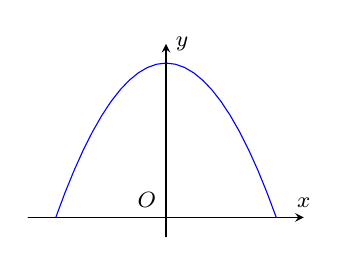
\begin{tikzpicture}[scale=.7,yscale=.7, font=\footnotesize, line join=round, line cap=round, >=stealth]
	\draw [->] (-2.5,0)--(2.5,0)node[above]{$x$}; % Hệ trục tọa độ
	\node at (0,0)[above left]{$O$};
	\draw [->] (0,-.5)--(0,4.5)node[right]{$y$};
	\draw [domain=-2:2, blue,] plot (\x, {04-(\x)^2});
	\end{tikzpicture}

}
	\loigiai{
		Dựa vào đồ thị, ta xây dựng được công thức của hàm số là $y=4-x^2$.\\
		Diện tích là $S=\displaystyle\int\limits_{-2}^2\left(4-x^2\right)\mathrm{\,d}x=\dfrac{28}{3}$.}
\end{ex}
\begin{ex}%[2D3K3-1]%Câu 28.
	\immini{
	Trong Công viên Toán học có những mảnh đất mang hình dáng khác nhau. Mỗi mảnh được trồng một loài hoa và nó được tạo thành bởi một trong những đường cong đẹp trong toán học. Ở đó có một mảnh đất mang tên Bernoulli, nó được tạo thành từ đường Lemmiscate có phương trình trong hệ tọa độ $Oxy$ là $16y^2=x^2\left(25-x^2\right)$ như hình vẽ bên. Tính diện tích $S$ của mảnh đất Bernoulli biết rằng mỗi đơn vị trong hệ tọa độ $Oxy$ tương ứng với chiều dài $1$ mét. 
	\choice
	{$S=\dfrac{125}{6}(m^2)$}
	{$S=\dfrac{125}{4}(m^2)$}
	{$S=\dfrac{250}{3}(m^2)$}
	{\True $S=\dfrac{125}{3}(m^2)$}
}{
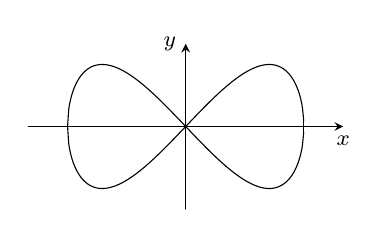
\begin{tikzpicture}[scale=.5,yscale=.7, font=\footnotesize, line join=round, line cap=round, >=stealth]
\def \xmin{-4} \def \xmax{4}
\def \ymin{-3} \def \ymax{3} 
\draw[-stealth] (\xmin,0)--(\xmax,0) node [below]{$x$};
\draw[-stealth] (0,\ymin)--(0,\ymax) node[left]{$y$};
%\node at (0,0)[above left]{$O$};
\def \f(#1){sqrt((#1)*(#1)*(9-(#1)*(#1))/4)}
\def \g(#1){-sqrt((#1)*(#1)*(9-(#1)*(#1))/4)}
\def \a{f(3)}
\draw[samples=200,smooth,domain=-3:3] plot (\x,{\f(\x)});
\draw[samples=200,smooth,domain=-3:3] plot (\x,{\g(\x)});
\draw (3,0)--(3,.2);\draw (3,0)--(3,-.2);
\end{tikzpicture}
}
	\loigiai{
		Vì tính đối xứng trụ nên diện tích của mảnh đất tương ứng với 4 lần diện tích của mảnh đất thuộc góc phần tư thứ nhất của hệ trục tọa độ $Oxy$.\\
		Từ giả thuyết bài toán, ta có $y=\pm\dfrac{1}{4}x\sqrt{25-x^2}$.\\
		Góc phần tư thứ nhất $y=\dfrac{1}{4}x\sqrt{25-x^2}; x\in[0; 5]$.\\
		Nên $S_{(I)}=\dfrac{1}{4}\displaystyle\int\limits_0^5 x\sqrt{25-x^2}\mathrm{\,d}x=\dfrac{125}{12}\Rightarrow S=\dfrac{125}{3}(m^2)$.}
\end{ex}
\begin{ex}%[2D3K3-1]%Câu 29.
	Gọi $(H)$ là hình phẳng giới hạn bởi đồ thị hàm số: $y=x^2-4x+4$, trục tung và trục hoành. Xác định $k$ để đường thẳng $(d)$ đi qua điểm $A(0; 4)$ có hệ số góc $k$ chia thành hai phần có diện tích bằng nhau. 
	\choice
	{$k=-4$}
	{$k=-8$}
	{\True $k=-6$}
	{$k=-2$}
	\loigiai{
		\immini{
			Phương trình hoành độ giao điểm của đồ thị hàm số $y=x^2-4x+4$ và trục hoành là\\
			$x^2-4x+4=0\Leftrightarrow x=2$.\\
			Diện tích hình phẳng $(H)$ giới hạn bởi đồ thị hàm số: $y=x^2-4x+4$, trục tung và trục hoành là\\ $S=\displaystyle\int\limits_0^2\left|x^2-4x+4\right|\mathrm{\,d}x=\displaystyle\int\limits_0^2\left(x^2-4x+4\right)\mathrm{\,d}x \\=\left(\dfrac{x^3}{3}-2x^2+4x\right)\bigg|_0^2=\dfrac{8}{3}$.\\
			Phương trình đường thẳng $(d)$ đi qua điểm $A(0;4)$ có hệ số góc $k$ có dạng: $y=kx+4$.\\
		}{
			\begin{tikzpicture}[scale=0.7, font=\footnotesize, line join=round, line cap=round,>=stealth]
			\def\a{1} \def\b{-4} \def\c{4} % Hệ số
			\def\xmin{-1.5} \def\xmax{5}
			\def\ymin{-1.5} \def\ymax{6}
			\draw[->] (\xmin,0)--(\xmax,0) node [below]{$x$};
			\draw[->] (0,\ymin)--(0,\ymax) node [right]{$y$};
			\node at (0,0) [below left]{$O$};
			\clip (\xmin+0.1,\ymin+0.1) rectangle (\xmax-0.5,\ymax-0.1);
			\draw[smooth,samples=300] plot(\x,{\a*(\x)^2+\b*(\x)+\c});
			\draw[smooth,samples=300] plot(\x,{-6*(\x)+4});
			\node at (1,-1)[right]{$d$};
			\fill (0,0) circle (1.0pt) (1,0) circle (1.0pt)node[below]{$1$} (2,0) circle (1.0pt)node[below]{$I$} (0,4) circle (1.0pt)node[right]{$4$};
			\fill[pattern=north east lines,opacity=0.5] (0,0)--(0,4)--(2/3,0)--cycle;
			\fill[pattern=north west lines,opacity=0.5] (0,4)--plot[domain=0:2](\x,{\a*(\x)^2+\b*(\x)+\c})--(2/3,0)--cycle;
			\node at (0,4)[left]{$A$};
			\fill (2/3,0) circle (1.0pt) node[below left]{$B$};
			\end{tikzpicture}
		}
	Gọi $B$ là giao điểm của $(d)$ và trục hoành. Khi đó $B\left(-\dfrac{4}{k}; 0\right)$.\\
	Đường thẳng $(d)$ chia $(H)$ thành hai phần có diện tích bằng nhau khi $B\in OI$ \\và $S_{\triangle OAB}=\dfrac{1}{2}S=\dfrac{4}{3}\Leftrightarrow\heva{&0 <-\dfrac{4}{k}<2\\&S_{\triangle OAB}=\dfrac{1}{2}OA\cdot OB=\dfrac{1}{2}\cdot 4\cdot\dfrac{-4}{k}=\dfrac{4}{3}}\Leftrightarrow\heva{&k <-2\\&k=-6}\Leftrightarrow k=-6$.
	}
\end{ex}	
\begin{ex}%[2D3K3-1]%Câu 30.
	\immini{
		Cho hàm số $y=x^4-3x^2+m$ có đồ thị $(C_m)$ với $m$ là tham số thực. Giả sử $(C_m)$ cắt trục $Ox$ tại bốn điểm phân biệt như hình vẽ. Gọi $S_1$, $S_2$ và $S_3$ là diện tích các miền gạch chéo được cho trên hình vẽ. Tìm $m$ để $S_1+S_2=S_3$. 
		\choice
		{$m=-\dfrac{5}{2}$}
		{$m=-\dfrac{5}{4}$}
		{$m=\dfrac{5}{2}$}
		{\True $m=\dfrac{5}{4}$}
	}{
		\begin{tikzpicture} [scale=.8,yscale=.7, font=\footnotesize, line join=round, line cap=round, >=stealth]
	\def \xmin{-3} \def \xmax{4}
	\def \ymin{-3} \def \ymax{5}
	\def \a{sqrt(3)}
	\draw[-stealth] (\xmin,0)--(\xmax,0) node [below]{$x$};
	\draw[-stealth] (0,\ymin)--(0,\ymax) node[left]{$y$};
	\path (0,0) circle(1pt) node[below left]{$O$};
	\draw [] (0,0.2)-|(0.2,0);
	%		\foreach \x in {-2,-1,1,2}
	%		\draw [shift={(\x,0)}](0pt,-1pt)--(0pt,1pt) node[above]{$\x$};	
%	\fill (-2,0) circle (1pt) node[below left] {$-2$} 
%	(-1,0) circle (1pt) node[below right] {$-1$} 
%	(1,0) circle (1pt) node[below left] {$1$}
%	(2,0) circle (1pt) node[below right] {$2$} 
%	;
	\def \f(#1){((#1)-1)*((#1)+1)*((#1)+2)*((#1)-2)}
	\fill[pattern=north west lines,opacity=8] plot[domain=-2:2](\x,{\f(\x)})--plot[domain=2:-2](\x,{0});
	\draw[samples=200,smooth,domain=-2.2:2.2] plot (\x,{\f(\x)});
	\clip (\xmin,\ymin) rectangle (\xmax,\ymax);
	\path 
	(-1.5,-1) node {$S_1$}
	(1.5,-1) node {$S_2$}
	(0.3,1.3) node {$S_3$};
	\end{tikzpicture}	
	}
	\loigiai{
		Giả sử $x=b$ là nghiệm dương lớn nhất của phương trình $x^4-3x^2+m=0$. \\Khi đó ta có
		$b^4-3b^2+m=0$ (1).\\
		Nếu xảy ra $S_1+S_2=S_3$ thì\\
		$\displaystyle\int\limits_0^b\left(x^4-3x^2+m\right)\mathrm{\,d}x=0\Rightarrow\dfrac{b^5}{5}-b^3+mb=0\Rightarrow\dfrac{b^4}{5}-b^2+m=0 \quad (2) \text{ (do } b>0 \text{)}$.\\
		Từ (1) và (2), trừ vế theo vế ta được $\dfrac{4}{5}b^4-2b^2=0\Rightarrow b^2=\dfrac{5}{2} \text{ (do } b>0 \text{)}$.\\
		Thay vào (1) ta được $m=\dfrac{5}{4}$.}
\end{ex}		

\Closesolutionfile{ans}
% \DAPAN
\inputansbox{10}{ans/ansCD2D3-3.1.1}

\Opensolutionfile{ans}[ans/ansCD2D3-3.1.2]
\begin{dang}{Ứng dụng tích phân tính diện tích hình phẳng giới hạn bởi $y=f(x),y=g(x), x=a,x=b$}
	\textbf{Phương pháp giải:}
	\immini
	{Diện tích hình phẳng giới hạn bởi hai đồ thị\\
		$(C_1)\colon y=f(x)$, $(C_2)\colon y=g(x)$ và hai đường thẳng $x=a$, $x=b$ được xác định bởi công thức: $$S=\displaystyle\int\limits_a^b\left|f(x)-g(x)\right|\mathrm{\,d}x$$.}
	{\begin{tikzpicture}[>=stealth, color=black, line width = 1pt, scale=.8]
		\draw[->] (-1,0)--(5,0) node[above]{$x$};
		\draw[->](0,-1) -- (0,4) node[right]{$y$};
		\draw(0,0) circle (1pt) node[below left]{$O$};
		\clip(-1,-1) rectangle (5,4);
		\draw[smooth,samples=100,domain=0.7:4.2] 
		plot(\x,{0.333333*(\x)^2-1.333333*(\x)+3.5});
		\draw[smooth,samples=100,domain=0.7:4.2] 
		plot(\x, {-0.25*(\x)^2+1.25*(\x)});
		\draw[pattern = north east lines, line width = 1pt,draw=none] (1,2.5)
		plot[domain=1:4] (\x,{0.333333*(\x)^2-1.333333*(\x)+3.5})--(4,3.5)--(4,1)-- plot[domain=4:1] (\x, {-0.25*(\x)^2+1.25*(\x)})--(1,1)--cycle;
		\draw(1,0)-- (1,2.5);
		\draw(4,0)-- (4,3.5);
		\begin{scriptsize}
		\draw[color=black] (1,-0.4) node {\normalsize $a$};
		\draw[color=black] (4,-0.4) node {\normalsize $b$};
		\draw[color=black] (2.2,3) node {\normalsize $y=f(x)$};
		\draw[color=black] (2.4,1) node {\normalsize $y=g(x)$};
		\end{scriptsize}
		\end{tikzpicture}} 
	Chú ý: Để phá bỏ dấu giá trị tuyệt đối ta thường làm như sau
	\begin{enumerate}[*]
		\item Giải phương trình: $f(x)=g(x)$ tìm nghiệm $x_1,x_2,\ldots,x_n\in(a;b)$, $\left(x_1<x_2 <\cdots <x_n\right)$.
		\item Tính:
		\allowdisplaybreaks
		\begin{eqnarray*}
			S&=&\displaystyle\int\limits_a^{x_1}\left|f(x)-g(x)\right|\mathrm{\,d}x+\displaystyle\int\limits_{x_1}^{x_2}\left|f(x)-g(x)\right|\mathrm{\,d}x+\cdots +\displaystyle\int\limits_{x_n}^b\left|f(x)-g(x)\right|\mathrm{\,d}x\\
			&=&\left|\displaystyle\int\limits_a^{x_1}\left(f(x)-g(x)\right)\mathrm{\,d}x\right|+\cdots +\left|\displaystyle\int\limits_{x_n}^b\left(f(x)-g(x)\right)\mathrm{\,d}x\right|.
		\end{eqnarray*}
	\end{enumerate}
	Ngoài cách trên, ta có thể dựa vào đồ thị để khử dấu giá trị tuyệt đối.
\end{dang}
\subsubsection{Các ví dụ}
\begin{vd}%Ví dụ 1.%[2D3B3-1]%[Don Lee]
	Tính diện tích hình phẳng giới hạn bởi đồ thị hàm số $y=2-x^2$ và $y=x$ và các đường thẳng $x=-2,x=1$.
	\choice
	{$5$}
	{$7$}
	{\True $\dfrac{9}{2}$}
	{$\dfrac{11}{2}$}
	\loigiai{
		\begin{enumerate}[*]
			\item Giải theo phương pháp tự luận:\\
			Diện tích hình phẳng $S=\displaystyle\int\limits_{-2}^1\left|-x^2-x+2\right|\mathrm{\,d}x=\left|\displaystyle\int\limits_{-2}^1 (-x^2-x+2){\,d}x\right|=\dfrac{9}{2}$.
			\item Giải theo phương pháp trắc nghiệm:\\
			Sử dụng máy tính Casio tính tích phân $\displaystyle\int\limits_{-2}^1\left|-x^2-x+2\right|\mathrm{\,d}x$.
		\end{enumerate}
	}
\end{vd}
\begin{vd}%Ví dụ 2.%[2D3B3-1]%[Don Lee]
	Diện tích hình phẳng giới hạn bởi các đồ thị hàm số $y=x^3+x;\,\,y=2x$ và các đường thẳng $x=-1;\,\,x=1$ được xác định bởi công thức 
	\choice
	{$S=\left|\displaystyle\int\limits_{-1}^1 (x-x^3)\mathrm{\,d}x\right|$}
	{$S=\displaystyle\int\limits_{-1}^1 (x-x^3)\mathrm{\,d}x$}
	{$S=\displaystyle\int\limits_{-1}^0 (x-x^3)\mathrm{\,d}x+\displaystyle\int\limits_0^1 (x^3-x)\mathrm{\,d}x$}
	{\True $S=\displaystyle\int\limits_{-1}^0 (x^3-x)\mathrm{\,d}x+\displaystyle\int\limits_0^1 (x-x^3)\mathrm{\,d}x$}
	\loigiai{
		\begin{enumerate}[*]
			\item Giải theo phương pháp tự luận:\\
			Phương trình hoành độ giao điểm của hai đồ thị: $x-x^3\Leftrightarrow\hoac{&x=0\\&x=\pm 1.}$
			\allowdisplaybreaks
			\begin{eqnarray*}
				S&=&\displaystyle\int\limits_{-1}^1\left|x-x^3\right|\mathrm{\,d}x=\displaystyle\int\limits_{-1}^0\left|x-x^3\right|\mathrm{\,d}x+\displaystyle\int\limits_0^1\left|x-x^3\right|\mathrm{\,d}x\\
				&=&\left|\displaystyle\int\limits_{-1}^0 (x-x^3)\mathrm{\,d}x\right|+\left|\displaystyle\int\limits_0^1 (x-x^3)\mathrm{\,d}x\right|\\
				&=&\displaystyle\int\limits_{-1}^0 (x^3-x)\mathrm{\,d}x+\displaystyle\int\limits_0^1 (x-x^3)\mathrm{\,d}x.
			\end{eqnarray*}
			\item Giải theo phương pháp trắc nghiệm:\\ $S=\displaystyle\int\limits_{-1}^1\left|x-x^3\right|\mathrm{\,d}x$ mà $x=0$ là nghiệm của PT hoành độ giao điểm của đồ thị hai hàm số nên đáp án $S=\left|\displaystyle\int\limits_{-1}^1 (x-x^3)\mathrm{\,d}x\right|$ và $S=\displaystyle\int\limits_{-1}^1 (x-x^3)\mathrm{\,d}x$ sai.\\
			Xét dấu biểu thức $x-x^3$ trên khoảng $(-1;0)$ bằng cách thay $x=-\dfrac{1}{2}$ vào biểu thức ta được $x-x^3<0$ nên đáp án $S=\displaystyle\int\limits_{-1}^0 (x-x^3)\mathrm{\,d}x+\displaystyle\int\limits_0^1 (x^3-x)\mathrm{\,d}x$ sai.
		\end{enumerate}
	}
\end{vd}
\begin{vd}%Ví dụ 3.%[2D3B3-1]%[Don Lee]
	Diện tích hình phẳng giới hạn bởi đồ thị hàm số $y=\dfrac{2x+1}{x-2}$; tiệm cận ngang và hai đường thẳng $x=3,x=e+2$ được tính bằng 
	\choice
	{$\displaystyle\int\limits_3^{e+2}\dfrac{2x+1}{x-2}\mathrm{\,d}x$}
	{\True $\displaystyle\int\limits_3^{e+2}\dfrac{5}{x-2}\mathrm{\,d}x$}
	{$\ln|x-2|\bigg|_3^{e+2}$}
	{$5-e$}
	\loigiai{
		\begin{enumerate}[*]
			\item Giải theo phương pháp tự luận:\\
			+ Tiệm cận ngang $y=2$.\\
			+ Đồ thị hàm số không cắt tiệm cận\\
			$\Rightarrow S=\displaystyle\int\limits_3^{e+2}\left|\dfrac{2x+1}{x-2}-2\right|\mathrm{\,d}x=\displaystyle\int\limits_3^{e+2}\left|\dfrac{5}{x-2}\right|\mathrm{\,d}x= 5\ln|x-2|\bigg|_3^{e+2}=5$.
			\item Giải theo phương pháp trắc nghiệm:\\
			Diện tích hình phẳng cần tìm giới hạn bởi đồ thị các hàm số $y=\dfrac{2x+1}{x-2}$ và $y=2$ nên\\ $S=\displaystyle\int\limits_3^{e+2}\left|\dfrac{2x+1}{x-2}-2\right|\mathrm{\,d}x$ suy ra loại đáp án $\displaystyle\int\limits_3^{e+2}\dfrac{2x+1}{x-2}\mathrm{\,d}x$. Rút gọn ta được đáp án đúng là $\displaystyle\int\limits_3^{e+2}\dfrac{5}{x-2}\mathrm{\,d}x$.
		\end{enumerate}
	}
\end{vd}
\begin{vd}%Ví dụ 4.%[2D3B3-1]%[Don Lee]
	\immini
	{Tính diện tích của $S$ phần hình phẳng giới hạn bởi đường Parabol đi qua gốc toạ độ và hai đoạn thẳng $AC$ và $BC$ như hình vẽ bên?
		\choice
		{$S=9$}
		{$S=\dfrac{10}{3}$}
		{\True $S=\dfrac{20}{3}$}
		{$S=\dfrac{25}{6}$}}
	{\begin{tikzpicture}[>=stealth, color=black, line width = 1pt, scale=.8]
		\draw[->] (-3,0)--(3,0) node[below]{\scriptsize $x$};
		\draw[->](0,-1) -- (0,5) node[right]{\scriptsize $y$};
		\draw(0,0) circle (1pt) node[below right]{\scriptsize $O$};
		\draw(-2,0) circle (1pt) node[below]{\scriptsize $-2$};
		\draw(-1,0) circle (1pt) node[below]{\scriptsize $-1$};
		\draw(1,0) circle (1pt) node[below]{\scriptsize $1$};
		\draw(2,0) circle (1pt) node[below]{\scriptsize $2$};
		\draw(0,2) circle (1pt) node[below left]{\scriptsize $2$};
		\draw(0,4) circle (1pt) node[below left]{\scriptsize $4$};
		\draw(-2,4) circle (1pt) node[left]{\scriptsize $A$};
		\draw(2,4) circle (1pt) node[right]{\scriptsize $B$};
		\draw(0,2) circle (1pt) node[above left]{\scriptsize $C$};
		\clip(-3,-1) rectangle (3,5);
		\draw[thick,samples=150,smooth,domain=-3:3] plot(\x,{(\x)^2});
		\draw[thick,samples=150,smooth,domain=-2:0] plot(\x,{-(\x)+2});
		\draw[thick,samples=150,smooth,domain=0:2] plot(\x,{(\x)+2});
		\draw[dashed] (-2,0)--(-2,4)--(2,4)--(2,0);
		\fill[pattern=north east lines]plot[domain=-2:0](\x,{(\x)^2})--plot[domain=0:-2](\x,{-(\x)+2})--cycle;
		\fill[pattern=north east lines]plot[domain=0:2](\x,{(\x)^2})--plot[domain=2:0](\x,{(\x)+2})--cycle;
		\end{tikzpicture}}
	\loigiai{
		\begin{enumerate}[*]
			\item Giải theo phương pháp tự luận:\\
			Dựa vào đồ thị đường Parabol có phương trình $y=x^2$.\\
			Đường thẳng chứa cạnh $BC$ có phương trình $y=x+2$.\\
			Diện tích hình phẳng cần tìm là $S=2\displaystyle\int\limits_0^2 (x+2-x^2)\mathrm{\,d}x=\dfrac{20}{3}$.
			\item Giải theo phương pháp trắc nghiệm:\\ $S=\dfrac{2}{3}\cdot 4\cdot 4-\dfrac{1}{2}\cdot 4\cdot 2=\dfrac{20}{3}$.
		\end{enumerate}
	}
\end{vd}
\subsubsection{Câu hỏi trắc nghiệm}
\begin{ex}%Câu 30.%[2D3Y3-1]%[Don Lee]
	Hình phẳng $(H)$ giới hạn bởi các đường $y=x^2$, $y=2x+3$ và hai đường $x=0$, $x=2$. Công thức nào sau đây tính diện tích hình phẳng $(H)$?
	\choice
	{$S=\displaystyle\int\limits_0^2\left(x^2-2x-3\right)\mathrm{\,d}x$}
	{\True $S=\displaystyle\int\limits_0^2\left|x^2-2x-3\right|\mathrm{\,d}x$}
	{$S=\displaystyle\int\limits_0^2\left|x^2-2x+3\right|\mathrm{\,d}x$}
	{$S=\displaystyle\int\limits_0^2\left|x^2+2x+3\right|\mathrm{\,d}x$}
	\loigiai{
		Giải theo phương pháp tự luận:\\
		Áp dụng lý thuyết: Diện tích hình phẳng giới hạn bởi hai đồ thị: $(C_1)\colon y=f(x)$, $(C_2)\colon y=g(x)$ và hai đường thẳng $x=a$, $x=b$ được xác định bởi công thức $S=\displaystyle\int\limits_a^b\left|f(x)-g(x)\right|\mathrm{\,d}x$.\\
		Khi đó diện tích hình phẳng $H=\displaystyle\int\limits_0^2\left|x^2-2x-3\right|\mathrm{\,d}x$.}
\end{ex}
\begin{ex}%Câu 31.%[2D3Y3-1]%[Don Lee]
	Diện tích hình phẳng giới hạn bởi đồ thị $y=f(x)$; $y=g(x)$, trục $Oy$ và đường thẳng $x=a,\,\,(a>0)$ là 
	\choice
	{$S=\displaystyle\int\limits_a^0\left|f(x)-g(x)\right|\mathrm{\,d}x$}
	{\True $S=\displaystyle\int\limits_0^a\left|f(x)-g(x)\right|\mathrm{\,d}x$}
	{$S=\displaystyle\int\limits_a^0\left|f(x)+g(x)\right|\mathrm{\,d}x$}
	{$S=\displaystyle\int\limits_0^a\left|f(x)+g(x)\right|\mathrm{\,d}x$}
	\loigiai{
		Giải theo phương pháp tự luận:\\
		Áp dụng lý thuyết: Diện tích hình phẳng giới hạn bởi hai đồ thị: $(C_1)\colon y=f(x)$, $(C_2)\colon y=g(x)$ và hai đường thẳng $x=a,x=b$ được xác định bởi công thức: $S=\displaystyle\int\limits_a^b\left|f(x)-g(x)\right|\mathrm{\,d}x$.\\
		Khi đó diện tích hình phẳng là $S=\displaystyle\int\limits_0^a\left|f(x)-g(x)\right|\mathrm{\,d}x$.}
\end{ex}
\begin{ex}%Câu 32.%[2D3B3-1]%[Don Lee]
	Gọi $S$ là diện tích hình phẳng giới hạn bởi các đường $y=x^2+5$, $y=6x$, $x=0$, $x=1$. Tính $S$. 
	\choice
	{$\dfrac{4}{3}$}
	{\True $\dfrac{7}{3}$}
	{$\dfrac{8}{3}$}
	{$\dfrac{5}{3}$}
	\loigiai{
		Giải theo phương pháp tự luận:\\
		Phương trình hoành độ giao điểm: $x^2+5=6x\Leftrightarrow x=5;x=1$.\\
		Diện tích hình phẳng cần tìm $S=\displaystyle\int\limits_0^1\left|x^2-6x+5\right|\mathrm{\,d}x=\dfrac{7}{3}$.\\
		Giải theo phương pháp trắc nghiệm:\\
		Sử dụng máy tính để nhận được kết quả của tích phân rồi so sánh với các đáp án.}
\end{ex}
\begin{ex}%Câu 33.%[2D3B3-1]%[Don Lee]
	Tính diện tích các hình phẳng giới hạn bởi đồ thị các hàm số $y=x^2-4, y=-x^2-2x$ và hai đường thẳng $x=-3, x=-2$. 
	\choice
	{$\dfrac{11}{6}$}
	{\True $\dfrac{11}{3}$}
	{$\dfrac{22}{3}$}
	{$\dfrac{19}{3}$}
	\loigiai{
		\immini
		{Giải theo phương pháp tự luận:\\
			Dựa vào hình vẽ ta thấy diện tích hình phẳng cần tìm là
			\allowdisplaybreaks
			\begin{eqnarray*}
				S&=&\displaystyle\int\limits_{-3}^{-2}\left|\left(x^2-4\right)-\left(-x^2-2x\right)\right|\mathrm{\,d}x\\
				&=&\displaystyle\int\limits_{-3}^{-2}\left[\left(x^2-4\right)-\left(-x^2-2x\right)\right]\mathrm{\,d}x\\
				&=&\displaystyle\int\limits_{-3}^{-2}\left(2x^2+2x-4\right)\mathrm{\,d}x\\ &=&\left(2\dfrac{x^3}{3}+2\dfrac{x^2}{2}-4x\right)\bigg|_{-3}^{-2}=\dfrac{11}{3}.
			\end{eqnarray*}
			Giải theo phương pháp trắc nghiệm:\\
			Sử dụng máy tính để nhận được kết quả của tích phân rồi so sánh với các đáp án.}
		{\begin{tikzpicture}[>=stealth, color=black, line width = 1pt, scale=.8]
			\draw[->] (-4,0)--(4,0) node[below]{$x$};
			\draw[->](0,-5) -- (0,6) node[right]{$y$};
			\draw(0,0) circle (1pt) node[below left]{$O$};
			\draw(-2,0) circle (1pt) node[shift={(-60:3mm)}]{$-2$};
			\draw(-3,0) circle (1pt) node[shift={(220:4mm)}]{$-3$};
			\fill(-3,4) node[right]{$y=x^2-4$}; 
			\fill(1/2,-3/2) node[right]{$y=-x^2-2x$};
			\clip(-4,-5) rectangle (4,6);
			\draw[thick,samples=150,smooth,domain=-4:4] plot(\x,{(\x)^2-4});
			\draw[thick,samples=150,smooth,domain=-4:4] plot(\x,{-(\x)^2-2*(\x)});
			\draw[thick,samples=150,smooth,domain=-4:4] (-3,-5)--(-3,6) (-2,-5)--(-2,6);
			\fill[pattern=north east lines]plot[domain=-3:-2](\x,{(\x)^2-4})--plot[domain=-2:-3](\x,{-(\x)^2-2*(\x)})--cycle; 
			\end{tikzpicture}}
		\noindent
		Nhận xét: Giải theo phương pháp tự luận ta có thể vẽ hình và nhìn thấy rõ trên đoạn $[-3;-2]$ đồ thị hàm số $y=x^2-4$ nằm trên đồ thị hàm số $y=-x^2-2x$ nên có thể phá dấu GTTĐ ngay; nếu không vẽ hình, ta đẩy dấu GTTĐ ra ngoài; còn trong trường hợp giải theo trắc nghiệm, ta chỉ cần bấm máy có cả dấu GTTĐ.}
\end{ex}
\begin{ex}%Câu 34.%[2D3B3-1]%[Don Lee]
	Tính diện tích hình phẳng giới hạn bởi các đường $y=x$, $y=x+\sin^2x$, $x=0$, $x=\pi$. 
	\choice
	{$S=\pi$}
	{$S=\pi-\dfrac{1}{2}$}
	{$S=\pi-1$}
	{\True $S=\dfrac{\pi}{2}$}
	\loigiai{
		Giải theo phương pháp tự luận:\\
		Hoành độ giao điểm của hai đồ thị là nghiệm của phương trình $x=x+\sin^2x\Leftrightarrow\sin^2x=0 \Leftrightarrow x=k\pi$ với $x \in [0;\pi]$.\\
		Vậy diện tích cần tìm là
		\allowdisplaybreaks
		\begin{eqnarray*}
			S&=&\displaystyle\int\limits_0^{\pi}\left|\sin^2x\right|\mathrm{\,d}x=\displaystyle\int\limits_0^{\pi}\sin^2x\mathrm{\,d}x =\displaystyle\int\limits_0^{\pi}\left(\dfrac{1-\cos 2x}{2}\right)\mathrm{\,d}x=\dfrac{1}{2}\left(\displaystyle\int\limits_0^{\pi}\mathrm{\,d}x-\displaystyle\int\limits_0^{\pi}\cos 2x\mathrm{\,d}x\right)\\
			&=&\dfrac{\pi}{2}-\dfrac{1}{4}\sin 2x\bigg|_0^{\pi}=\dfrac{\pi}{2}.
		\end{eqnarray*}
		Giải theo phương pháp trắc nghiệm:\\
		Sử dụng máy tính để tính tích phân $S=\displaystyle\int\limits_0^{\pi}\left|\sin^2x\right|\mathrm{\,d}x$.}
\end{ex}
\begin{ex}%Câu 35.%[2D3B3-1]%[Don Lee]
	Diện tích hình phẳng giới hạn bởi $y=x^2-4$, $y=-x^2-2x$ và $x=-2$ bằng 
	\choice
	{\True $\dfrac{11}{3}$}
	{$3$}
	{$\dfrac{7}{3}$}
	{$\dfrac{5}{3}$}
	\loigiai{
		Giải theo phương pháp tự luận:\\
		Hoành độ giao điểm của hai đồ thị là nghiệm của phương trình:\\
		$x^2-4=-x^2-2x\Leftrightarrow 2x^2+2x-4=0\Leftrightarrow\hoac{&x=1\\&x=-2.}$ \\
		Khi đó
		\allowdisplaybreaks
		\begin{eqnarray*}
			S&=&\displaystyle\int\limits_{-3}^{-2}\left|x^2-4-\left(-x^2-2x\right)\right|\mathrm{\,d}x =\displaystyle\int\limits_{-3}^{-2}\left|2x^2+2x-4\right|\mathrm{\,d}x=2\displaystyle\int\limits_{-3}^{-2}\left(x^2+x-2\right)\mathrm{\,d}x\\
			&=&2\left(\dfrac{1}{3}x^3+\dfrac{1}{2}x^2-2x\right)\bigg|_{-3}^{-2}=\dfrac{11}{3}.
		\end{eqnarray*}
		Giải theo phương pháp trắc nghiệm:\\
		Sử dụng máy tính để nhận được kết quả của tích phân rồi so sánh với các đáp án.}
\end{ex}
\begin{ex}%Câu 36.%[2D3B3-1]%[Don Lee]
	Tính diện tích hình phẳng giới hạn bởi hàm số $y=x^4-4x^2+4$, $y=x^2$, trục tung và đường thẳng $x=1$. 
	\choice
	{$\dfrac{38}{25}$}
	{$\dfrac{38}{35}$}
	{\True $\dfrac{38}{15}$}
	{$\dfrac{38}{5}$}
	\loigiai{
		\immini
		{Giải theo phương pháp tự luận:\\
			Diện tích hình phẳng cần tìm là:\\
			$S=\displaystyle\int\limits_0^1\left|x^4-4x^2+4-x^2\right|\mathrm{\,d}x =\displaystyle\int\limits_0^1\left|x^4-5x^2+4\right|\mathrm{\,d}x$.\\
			Vì $x^4-5x^2+4=\left(x^2-1\right)\left(x^2-4\right)\geq 0$, \quad $\forall x\in[0;1]$.\\
			nên $S=\displaystyle\int\limits_0^1\left(x^4-5x^2+4\right)\mathrm{\,d}x =\left(\dfrac{x^5}{5}-\dfrac{5x^3}{3}+4x\right)\bigg|_0^1=\dfrac{1}{5}-\dfrac{5}{3}+4 =\dfrac{38}{15}$.\\
			Giải theo phương pháp trắc nghiệm:\\
			Sử dụng máy tính để tính $\displaystyle\int\limits_0^1\left|x^4-4x^2+4-x^2\right|\mathrm{\,d}x$.}
		{\begin{tikzpicture}[>=stealth, color=black, line width = 1pt, scale=.8]
			\draw[->] (-3,0)--(3,0) node[below]{$x$};
			\draw[->](0,-1) -- (0,6) node[right]{$y$};
			\draw(0,0) circle (1pt) node[below left]{$O$};
			\draw(1,0) circle (1pt) node[shift={(240:2mm)}]{$1$};
			\fill(-11/5,9/2) node[right, blue]{\scriptsize $y=x^4-4x^2+4$}; 
			\fill(2,5) node[right,red]{\scriptsize $y=x^2$};
			\clip(-3,-1) rectangle (3,6);
			\draw[thick,red,samples=150,smooth,domain=-3:3] plot(\x,{(\x)^2});
			\draw[thick,blue,samples=150,smooth,domain=-3:3] plot(\x,{(\x)^4-4*(\x)^2+4});
			\draw[thick,green,samples=150,smooth,domain=-3:3] (1,-1)--(1,6);
			\fill[pattern=north east lines]plot[domain=0:1](\x,{(\x)^4-4*(\x)^2+4})--plot[domain=1:0](\x,{(\x)^2})--cycle; 
			\end{tikzpicture}}
	}
\end{ex}
\begin{ex}%Câu 37.%[2D3B3-1]%[Don Lee]
	Tính diện tích của những hình phẳng được giới hạn bởi các đường cong $y=\mathrm{e}^x$, $y=\mathrm{e}^{-x}$, $x=-\ln 2$, $x=\ln 2$. 
	\choice
	{$\dfrac{3}{4}$}
	{$\dfrac{1}{2}$}
	{$2$}
	{\True $1$}
	\loigiai{
		\immini
		{Giải theo phương pháp tự luận:\\
			Vì tính đối xứng qua $Oy$, nên ta chỉ cần tính\\
			$S_1=\displaystyle\int\limits_0^{\ln 2}\left(\mathrm{e}^x-\mathrm{e}^{-x}\right)\mathrm{\,d}x =\displaystyle\int\limits_0^{\ln 2}\mathrm{e}^x\mathrm{\,d}x-\displaystyle\int\limits_0^{\ln 2}\mathrm{e}^{-x}\mathrm{\,d}x =\mathrm{e}^x\bigg|_0^{\ln 2}+\mathrm{e}^u\bigg|_0^{-\ln 2} =2-1+\left(\dfrac{1}{2}-1\right)=\dfrac{1}{2}$.\\
			Do đó diện tích cần tính là $S=2\cdot S_1=1$.\\
			Giải theo phương pháp trắc nghiệm:\\
			Sử dụng máy tính để tính tích phân $S_1=\displaystyle\int\limits_0^{\ln 2}\left(\mathrm{e}^x-\mathrm{e}^{-x}\right)\mathrm{\,d}x$.}
		{\begin{tikzpicture}[>=stealth, color=black, line width = 1pt, scale=.7]
			\draw[->] (-2,0)--(2,0) node[below]{\scriptsize $x$};
			\draw[->](0,-1) -- (0,4) node[left]{\scriptsize $y$};
			\draw(0,0) circle (1pt) node[below left]{\scriptsize $O$};
			\draw(1,0) circle (1pt) node[below]{\scriptsize $1$};
			\fill(-2,3) node[right, blue]{\scriptsize $y=\mathrm{e}^{-x}$};
			\fill(2/3,7/2) node[right,red]{\scriptsize $y=\mathrm{e}^x$};
			\fill(1,0) node[below left]{\tiny $\ln 2$};
			\fill(-4/3,0) node[below]{\tiny $-\ln2$};
			\clip(-2,-1) rectangle (2,4);
			\draw[thick,red,samples=150,smooth,domain=-2:2] plot(\x,{(2.718)^(\x)});
			\draw[thick,blue,samples=150,smooth,domain=-2:2] plot(\x,{(2.718)^(-\x)});
			\draw[thick,green,samples=150,smooth,domain=-2:2] (0.6931,-1)--(0.6931,4);
			\draw[thick,green,samples=150,smooth,domain=-2:2] (-0.6931,-1)--(-0.6931,4);
			\fill[pattern=north east lines]plot[domain=-0.6931:0.6931](\x,{(2.718)^(-\x)})--plot[domain=0.6931:-0.6931](\x,{(2.718)^(\x)})--cycle; 
			\end{tikzpicture}}
	}
\end{ex}
\begin{ex}%Câu 38.%[2D3B3-1]%[Don Lee]
	Tính diện tích hình phẳng được giới hạn bởi các đường $y=x^3,y=2-x^2,x=0$. 
	\choice
	{$-\dfrac{17}{12}$}
	{$\dfrac{12}{17}$}
	{$0$}
	{\True $\dfrac{17}{12}$}
	\loigiai{
		Giải theo phương pháp tự luận:\\
		Ta có $x^3=2-x^2\Leftrightarrow x^3+x^2-2=0\Leftrightarrow x=1$.\\
		Suy ra $S=\displaystyle\int\limits_0^1\left|x^3+x^2-2\right|\mathrm{\,d}x=\left(\dfrac{x^4}{4}+\dfrac{x^3}{3}-2x\right)\bigg|_0^1=\dfrac{17}{12}$.\\
		Giải theo phương pháp trắc nghiệm:\\
		Sử dụng máy tính để tính tích phân $S=\displaystyle\int\limits_0^1\left|x^3+x^2-2\right|\mathrm{\,d}x$.}
\end{ex}
\begin{ex}%Câu 39.%[2D3B3-1]%[Don Lee]
	Diện tích hình phẳng giới hạn bởi các đồ thị hàm số $y=x^3-x, y=2x$ và các đường thẳng $x=-1,x=1$ được xác định bởi công thức 
	\choice
	{$S=\left|\displaystyle\int\limits_{-1}^1\left(3x-x^3\right)\mathrm{\,d}x\right|$}
	{$S=\displaystyle\int\limits_{-1}^0\left(3x-x^3\right)\mathrm{\,d}x+\displaystyle\int\limits_0^1\left(x^3-3x\right)\mathrm{\,d}x$}
	{$S=\displaystyle\int\limits_{-1}^1\left(3x-x^3\right)\mathrm{\,d}x$}
	{\True $S=\displaystyle\int\limits_{-1}^0\left(x^3-3x\right)\mathrm{\,d}x+\displaystyle\int\limits_0^1\left(3x-x^3\right)\mathrm{\,d}x$}
	\loigiai{
		Giải theo phương pháp tự luận:\\
		Xét phương trình hoành độ giao điểm của hai đồ thị:\\ $x^3-x=2x\Leftrightarrow x^3-x=0\Leftrightarrow x=0$ (chỉ xét trên $(-1; 1)$).\\
		Với $x\in(-1;0)$ thì $x^3-3x>0;$ với $x\in(0;1)$ thì $x^3-3x<0$.\\
		Diện tích cần tìm là $S=\displaystyle\int\limits_{-1}^1\left|x^3-3x\right|\mathrm{\,d}x=\displaystyle\int\limits_{-1}^0\left(x^3-3x\right)\mathrm{\,d}x+\displaystyle\int\limits_0^1\left(3x-x^3\right)\mathrm{\,d}x$.\\
		Giải theo phương pháp trắc nghiệm:\\ $S=\displaystyle\int\limits_{-1}^1\left|x^3-3x\right|\mathrm{\,d}x$\\
		Mà $x=0$ là nghiệm của PT hoành độ giao điểm của đồ thị hai hàm số nên đáp án $S=\left|\displaystyle\int\limits_{-1}^1\left(3x-x^3\right)\mathrm{\,d}x\right|$ và $S=\displaystyle\int\limits_{-1}^0\left(3x-x^3\right)\mathrm{\,d}x+\displaystyle\int\limits_0^1\left(x^3-3x\right)\mathrm{\,d}x$ sai.\\
		Xét dấu biểu thức $x^3-3x$ trên khoảng $(-1;0)$ bằng cách thay $x=-\dfrac{1}{2}$ vào biểu thức ta được $x^3-3x>0$ nên đáp án $S=\displaystyle\int\limits_{-1}^1\left(3x-x^3\right)\mathrm{\,d}x$ sai.}
\end{ex}
\begin{ex}%Câu 40.%[2D3B3-1]%[Don Lee]
	Tính diện tích hình phẳng giới hạn bởi đồ thị $(C)\colon y=\dfrac{x+2}{x+1}$, tiệm cận ngang của $(C)$, trục tung và đường thẳng $x=2$. 
	\choice
	{\True $\ln 2$}
	{$\dfrac{1}{8}\ln\dfrac{1}{4}$}
	{$\ln\dfrac{1}{2}$}
	{$\dfrac{1}{4}\ln\dfrac{1}{2}$}
	\loigiai{
		Giải theo phương pháp tự luận:\\
		Ta có $(C)\colon y=\dfrac{x+2}{x+1}$ có tiệm cận ngang là $y=1$.\\
		Diện tích: $S=\left|\displaystyle\int\limits_0^2\left(\dfrac{x+2}{x+1}-1\right)\mathrm{\,d}x\right|=\left|\displaystyle\int\limits_0^2\dfrac{1}{x+1}\mathrm{\,d}x\right|=\left|\ln (x+1)\bigg|_0^1\right|=\ln 2$.\\
		Giải theo phương pháp trắc nghiệm:\\
		Sử dụng máy tính để tính tích phân $\displaystyle\int\limits_0^2\left|\dfrac{x+2}{x+1}-1\right|\mathrm{\,d}x$.}
\end{ex}
\begin{ex}%Câu 41.%[2D3B3-1]%[Don Lee]
	Tính diện tích hình phẳng giới hạn bởi đường cong $(C)\colon y=\dfrac{2x+1}{x+1},$ tiệm cận ngang của $(C)$ và hai đường thẳng $x=1, x=3$. 
	\choice
	{\True $S=\ln 2$}
	{$S=4\ln 2$}
	{$S=1+\ln 2$}
	{$S=1$}
	\loigiai{
		Giải theo phương pháp tự luận:\\
		Ta có $(C)\colon y=\dfrac{2x+1}{x+1}$ có tiệm cận ngang là $y=2$.\\
		Diện tích: $S=\left|\displaystyle\int\limits_1^3\left(\dfrac{2x+1}{x+1}-2\right)\mathrm{\,d}x\right|=\left|\displaystyle\int\limits_1^3\dfrac{-1}{x+1}\mathrm{\,d}x\right|=\left|\ln (x+1)\bigg|_1^3\right|=\ln 2$.\\
		Giải theo phương pháp trắc nghiệm:\\
		Sử dụng máy tính để tính tích phân $\left|\displaystyle\int\limits_1^3\left(\dfrac{2x+1}{x+1}-2\right)\mathrm{\,d}x\right|$.}
\end{ex}
\begin{ex}%Câu 42.%[2D3B3-1]%[Don Lee]
	Diện tích hình phẳng giới hạn bởi các đường $(P)\colon y=x^2-2x+2,$ trục tung, tiếp tuyến của $(P)$ tại $M(3;5)$ là 
	\choice
	{$S=3$}
	{$S=6$}
	{$S=7$}
	{\True $S=9$}
	\loigiai{
		\immini
		{Giải theo phương pháp tự luận:\\
			Ta có $y’=2x-2\Rightarrow y’(3)=4$.\\
			Phương trình tiếp tuyến tại $M$ là: $y-5=4(x-3)$ hay $y=4x-7$.\\
			Diện tích cần tìm là
			\allowdisplaybreaks
			\begin{eqnarray*} S&=&\displaystyle\int\limits_0^3\left[(x-2x+2)-(4x-7)\right]\mathrm{\,d}x=\displaystyle\int\limits_0^3\left(x^2-6x+9\right)\mathrm{\,d}x=\displaystyle\int\limits_0^3(x-3)^2\mathrm{\,d}x\\
				&=&\dfrac{(x-3)^3}{3}\bigg|_0^3=9.
			\end{eqnarray*}
			Giải theo phương pháp trắc nghiệm:\\
			Sử dụng máy tính để tính tích phân $S=\displaystyle\int\limits_0^3\left[(x-2x+2)-(4x-7)\right]\mathrm{\,d}x$.}
		{\begin{tikzpicture}[>=stealth, color=black, line width = 1pt, scale=0.7]
			\draw[->] (-2,0)--(4,0) node[below]{$x$};
			\draw[->](0,-8) -- (0,8) node[left]{$y$};
			\draw(0,0) circle (1pt) node[shift={(220:3mm)}]{$O$};
			\draw(3,5) circle (1pt) node[right]{$M(3;5)$};
			\draw(0,-7) circle (1pt) node[left]{$-7$};
			\fill(-3/2,7) node[right]{\scriptsize $y=x^2-2x+2$};
			\fill(1,-3) node[right]{\scriptsize $y=4x-7$};
			\clip(-2,-8) rectangle (4,8);
			\draw[thick,samples=150,smooth,domain=-2:4] plot(\x,{(\x)^2-2*(\x)+2});
			\draw[thick,samples=150,smooth,domain=-1:4] plot(\x,{4*(\x)-7});
			\fill[pattern=north east lines]plot[domain=0:3](\x,{(\x)^2-2*(\x)+2})--plot[domain=3:0](\x,{4*(\x)-7})--cycle;
			\end{tikzpicture}}
	}
\end{ex}
\begin{ex}%Câu 43.%[2D3B3-2]%[Don Lee]
	\immini
	{Sơ đồ ở bên dưới phác thảo của một khung cửa sổ. Diện tích của cửa sổ được tính bằng công thức nào sau đây?
		\choice
		{\True $S=\displaystyle\int\limits_{-\tfrac{1}{2}}^{\tfrac{1}{2}}\left(\dfrac{5}{2}-4x^2\right)\mathrm{\,d}x$}
		{$S=\displaystyle\int\limits_{-\tfrac{1}{2}}^{\tfrac{1}{2}}\left|\dfrac{5}{2}-2x^2\right|\mathrm{\,d}x$}
		{$S=\displaystyle\int\limits_{-\tfrac{1}{2}}^{\tfrac{1}{2}} 2x^2\mathrm{\,d}x$}
		{$S=\displaystyle\int\limits_{-\tfrac{1}{2}}^{\tfrac{1}{2}}\left(1-4x^2\right)\mathrm{\,d}x$}}
	{\begin{tikzpicture}[>=stealth, color=black, line width = 1pt, scale=1]
		\draw[->] (-1,0)--(3/2,0) node[below]{\scriptsize $x$};
		\draw[->](0,-1) -- (0,3) node[left]{\scriptsize $y$};
		\draw(0,0) circle (1pt) node[shift={(220:2mm)}]{\scriptsize $O$};
		\draw(1/2,0) circle (1pt) node[below]{\scriptsize $\tfrac{1}{2}$};
		\draw(-1/2,0) circle (1pt) node[below]{\scriptsize $-\tfrac{1}{2}$};
		\fill(1/5,5/2) node[right]{\tiny $y=\dfrac{5}{2}-2x^2$};
		\fill(1/5,1/4) node[right]{\tiny $y=2x^2$};
		\clip(-1,-1) rectangle (3/2,3);
		\draw[thick,samples=150,smooth,domain=-1/2:1/2] plot(\x,{2*(\x)^2});
		\draw[thick,samples=150,smooth,domain=-1/2:1/2] plot(\x,{5/2-2*(\x)^2});
		\draw (-1/2,1/2)--(-1/2,2) (1/2,1/2)--(1/2,2);
		\draw[dashed] (-1/2,0)--(-1/2,1/2)  (1/2,0)--(1/2,1/2);
		\end{tikzpicture}}
	\loigiai{
		Giải theo phương pháp tự luận:\\
		Dựa vào đồ thị ta thấy trên đoạn $\left[-\dfrac{1}{2};\dfrac{1}{2}\right]$ thì đồ thị hàm số $y_1=\dfrac{5}{2}-2x^2$ nằm phía trên đồ thị hàm số $y_2=2x^2$.\\
		Do đó $S=\displaystyle\int\limits_{-\tfrac{1}{2}}^{\tfrac{1}{2}}(y_1-y_2)\mathrm{\,d}x=\displaystyle\int\limits_{-\tfrac{1}{2}}^{\tfrac{1}{2}}\left(\dfrac{5}{2}-2x^2-2x^2\right)\mathrm{\,d}x=\displaystyle\int\limits_{-\tfrac{1}{2}}^{\tfrac{1}{2}}\left(\dfrac{5}{2}-4x^2\right)\mathrm{\,d}x$.\\
		Giải theo phương pháp trắc nghiệm:\\
		Sử dụng máy tính để tính tích phân $S=\displaystyle\int\limits_{-\tfrac{1}{2}}^{\tfrac{1}{2}}\left(\dfrac{5}{2}-2x^2-2x^2\right)\mathrm{\,d}x$.}
\end{ex}
\begin{ex}%Câu 44.%[2D3B3-1]%[Don Lee]
	Tính diện tích hình phẳng giới hạn bởi Đồ thị các hàm số $y=\ln x$, $y=-\ln x$ và $x=e$. 
	\choice
	{\True $2$}
	{$\dfrac{5}{2}$}
	{$\ln e$}
	{$2\ln e$}
	\loigiai{
		Giải theo phương pháp tự luận: Hoành độ giao điểm của hai đồ thị là nghiệm của phương trình: $\ln x=-\ln x\Leftrightarrow 2\ln x=0\Leftrightarrow\ln x=0\Leftrightarrow x=1$.\\
		Khi đó: $S=\displaystyle\int\limits_1^e|\ln x+\ln x|\mathrm{\,d}x = 2\displaystyle\int\limits_1^e\ln x\cdot\mathrm{\,d}x$.\\
		Đặt: $\heva{&u=\ln x\\&\mathrm{\,d}v=\mathrm{\,d}x}\Leftrightarrow\heva{&\mathrm{\,d}u=\dfrac{\mathrm{\,d}x}{x}\\&v=x}\Leftrightarrow S=2\left(x\cdot\ln x\bigg|_1^e-\displaystyle\int\limits_1^e\mathrm{\,d}x\right) = 2\left(e- x\bigg|_1^e\right) =2$.\\
		Giải theo phương pháp trắc nghiệm: Sử dụng máy tính để tính tích phân $\displaystyle\int\limits_1^e|\ln x+\ln x|\mathrm{\,d}x$.}
\end{ex}
\begin{ex}%Câu 45.%[2D3B3-1]%[Don Lee]
	Tính diện tích hình phẳng giới hạn bởi parabol $y=x^2+1$, tiếp tuyến với đường này tại điểm $M(2;5)$ và trục $Oy$. 
	\choice
	{$\dfrac{5}{6}$}
	{$\dfrac{9}{11}$}
	{\True $\dfrac{8}{3}$}
	{$\dfrac{5}{2}$}
	\loigiai{
		\immini
		{Giải theo phương pháp tự luận:\\
			Ta có $y’=f’(x)=2x\Rightarrow f’(2)=4$.\\
			Phương trình tiếp tuyến tại tiếp điểm $M(2;5)\in(P)$ là\\ $y-5=4(x-2)\Leftrightarrow y=4x-3$.\\
			$S=\displaystyle\int\limits_0^2\left(x^2+1-4x+3\right)\mathrm{\,d}x=\displaystyle\int\limits_0^2\left(x^2-4x+4\right)\mathrm{\,d}x=\displaystyle\int\limits_0^2(x-2)^2\mathrm{\,d}x$.\\
			Đặt $u=x-2\Rightarrow\mathrm{\,d}u=\mathrm{\,d}x$.\\
			Đổi cận $x=2\Rightarrow u=0$; $x=0\Rightarrow u=-2$.\\
			Do đó: $S=\displaystyle\int\limits_{-2}^0 u^2\mathrm{\,d}u=\dfrac{u^3}{3}\bigg|_{-2}^0=\dfrac{8}{3}$ đvdt.\\
			Giải theo phương pháp trắc nghiệm:\\
			Sử dụng máy tính để tính tích phân $S=\displaystyle\int\limits_0^2\left(x^2+1-4x+3\right)\mathrm{\,d}x$.}
		{\begin{tikzpicture}[>=stealth, color=black, line width = 1pt, scale=0.7]
			\draw[->] (-5/2,0)--(3,0) node[below]{$x$};
			\draw[->](0,-4) -- (0,6) node[left]{$y$};
			\draw(0,0) circle (1pt) node[shift={(220:3mm)}]{$O$};
			\draw(2,5) circle (1pt) node[right]{$M(2;5)$};
			\draw(0,-3) circle (1pt) node[left]{$-3$};
			\fill(-9/4,16/3) node[right]{\scriptsize $y=x^2+1$};
			\fill(2/3,-3/2) node[right]{\scriptsize $y=4x-3$};
			\clip(-5/2,-4) rectangle (3,6);
			\draw[thick,samples=150,smooth,domain=-5/2:5/2] plot(\x,{(\x)^2+1});
			\draw[thick,samples=150,smooth,domain=-1:5/2] plot(\x,{4*(\x)-3});
			\fill[pattern=north east lines]plot[domain=0:2](\x,{(\x)^2+1})--plot[domain=2:0](\x,{4*(\x)-3})--cycle;
			\end{tikzpicture}}
	}
\end{ex}
\begin{ex}%Câu 46.%[2D3B3-1]%[Don Lee]
	Tính diện tích hình phẳng giới hạn bởi đồ thị các hàm số $y=x\sqrt{1+x^2}$, $y=\dfrac{x}{\sqrt{1+x^2}}$ và hai đường thẳng $x=0$, $x=\sqrt{3}$. 
	\choice
	{$\dfrac{1}{3}$}
	{\True $\dfrac{4}{3}$}
	{$2$}
	{$1$}
	\loigiai{
		Giải theo phương pháp tự luận:\\
		Ta có: $S=\displaystyle\int\limits_0^{\sqrt{3}}\left|x\sqrt{1+x^2}-\dfrac{x}{\sqrt{1+x^2}}\right|\mathrm{\,d}x =\displaystyle\int\limits_0^{\sqrt{3}}\left|\dfrac{x(1+x^2)-x}{\sqrt{1+x^2}}\right|\mathrm{\,d}x =\displaystyle\int\limits_0^{\sqrt{3}}\dfrac{x^3}{\sqrt{x^2+1}}\mathrm{\,d}x$.\\
		Tới đây, để tính tích phân ta có thể trình bày theo các cách sau
		\begin{enumerate}[.]
			\item Cách 1: Đặt $u=\sqrt{x^2+1}$, suy ra: $u^2=x^2+1\Leftrightarrow 2u\mathrm{\,d}u=2x\mathrm{\,d}x\Leftrightarrow u\mathrm{\,d}u=x\mathrm{\,d}x$.\\
			Đổi cận: Với $x=0$ thì $u=1$; với $x=\sqrt{3}$ thì $u=2$.\\
			Từ đó $S=\displaystyle\int\limits_1^2\dfrac{(u^2-1)u\mathrm{\,d}u}{u}=\displaystyle\int\limits_1^2 (u^2-1)\mathrm{\,d}u=\left(\dfrac{u^3}{3}-u\right)\bigg|_1^2=\dfrac{4}{3}$.
			\item Cách 2: Đặt $u=x^2+1$, suy ra $\mathrm{\,d}u=2x\mathrm{\,d}x$.\\
			Đổi cận: Với $x=0$ thì $u=1$ với $x=\sqrt{3}$ thì $u=4$.\\
			Từ đó: S = $S=\dfrac{1}{2}\displaystyle\int\limits_1^4\dfrac{(u-1)\mathrm{\,d}u}{\sqrt{u}} =\displaystyle\int\limits_1^4\left(\dfrac{\sqrt{u}}{2}-\dfrac{1}{2\sqrt{u}}\right)\mathrm{\,d}u =\left(\dfrac{1}{3}u^{\tfrac{3}{2}}-\sqrt{u}\right)\bigg|_1^4 =\dfrac{4}{3}$.
		\end{enumerate}
		Giải theo phương pháp trắc nghiệm:\\
		Sử dụng máy tính để tính tích phân $S=\displaystyle\int\limits_0^{\sqrt{3}}\left|x\sqrt{1+x^2}-\dfrac{x}{\sqrt{1+x^2}}\right|\mathrm{\,d}x$.}
\end{ex}
\begin{ex}%Câu 47.%[2D3B3-1]%[Don Lee]
	Cho hai hàm số $f$ và $g$ liên tục trên đoạn $[a;b]$ với $(a<b)$. Kí hiệu $S_1$ là diện tích hình phẳng giới hạn bởi các đường $y=2f(x)$, $y=2g(x)$, $x=a$, $x=b$. $S_2$ là diện tích hình phẳng giới hạn bởi các đường $y=f(x)-2$, $y=g(x)-2$, $x=a$, $x=b$.\\
	Chọn khẳng định đúng trong $4$ khẳng định sau: 
	\choice
	{$S_1=S_2$}
	{\True $S_1=2S_2$}
	{$S_1=2S_2-2$}
	{$S_1=2S_2+2$}
	\loigiai{
		Giải theo phương pháp tự luận:\\
		Ta có $S_1=\displaystyle\int\limits_a^b\left|2f(x)-2g(x)\right|\mathrm{\,d}x=2\displaystyle\int\limits_a^b\left|f(x)-g(x)\right|\mathrm{\,d}x$.\\
		$S_2=\displaystyle\int\limits_a^b\left|f(x)-2-[g(x)-2]\right|\mathrm{\,d}x=\displaystyle\int\limits_a^b\left|f(x)-g(x)\right|\mathrm{\,d}x$.\\
		Vậy $S_1=2S_2$.}
\end{ex}
\begin{ex}%Câu 48.%[2D3B3-1]%[Don Lee]
	\immini
	{Tính diện tích $S$ của phần hình phẳng giới hạn bởi đường Parabol đi qua gốc tọa độ và hai đoạn thẳng $AC$ và $BC$ như hình vẽ bên. 
		\choice
		{$S=\dfrac{25}{6}$}
		{$S=\dfrac{20}{3}$}
		{\True $S=\dfrac{10}{3}$}
		{$S=9$}}
	{\begin{tikzpicture}[>=stealth, color=black, line width = 1pt, scale=.8]
		\draw[->] (-3,0)--(3,0) node[below]{\scriptsize $x$};
		\draw[->](0,-1) -- (0,5) node[right]{\scriptsize $y$};
		\draw(0,0) circle (1pt) node[below right]{\scriptsize $O$};
		\draw(-2,0) circle (1pt) node[below]{\scriptsize $-2$};
		\draw(-1,0) circle (1pt) node[below]{\scriptsize $-1$};
		\draw(1,0) circle (1pt) node[below]{\scriptsize $1$};
		\draw(2,0) circle (1pt) node[below]{\scriptsize $2$};
		\draw(0,2) circle (1pt) node[below left]{\scriptsize $2$};
		\draw(0,4) circle (1pt) node[below left]{\scriptsize $4$};
		\draw(-2,4) circle (1pt) node[left]{\scriptsize $A$};
		\draw(2,4) circle (1pt) node[right]{\scriptsize $B$};
		\draw(0,2) circle (1pt) node[above left]{\scriptsize $C$};
		\clip(-3,-1) rectangle (3,5);
		\draw[thick,samples=150,smooth,domain=-3:3] plot(\x,{(\x)^2});
		\draw[thick,samples=150,smooth,domain=-2:0] plot(\x,{-(\x)+2});
		\draw[thick,samples=150,smooth,domain=0:2] plot(\x,{(\x)+2});
		\draw[dashed] (-2,0)--(-2,4)--(2,4)--(2,0);
		\fill[pattern=north east lines]plot[domain=-2:0](\x,{(\x)^2})--plot[domain=0:-2](\x,{-(\x)+2})--cycle;
		\fill[pattern=north east lines]plot[domain=0:2](\x,{(\x)^2})--plot[domain=2:0](\x,{(\x)+2})--cycle;
		\end{tikzpicture}}
	\loigiai{
		Giải theo phương pháp tự luận:\\
		Gọi $S_1$ là diện tích hình phẳng giới hạn bởi các đường $y=x^2$, $y=x+2$, $x=0$, $x=2$ \\
		Suy ra $S_1=\displaystyle\int\limits_0^2\left(x+2-x^2\right)\mathrm{\,d}x=\left(\dfrac{x^2}{2}+2x-\dfrac{x^3}{3}\right)\bigg|_0^2=\dfrac{2^2}{2}+2\cdot 2-\dfrac{2^3}{3}=\dfrac{10}{3} $.\\
		Khi đó diện tích hình phẳng phần gạch chéo là $S=2\cdot S_1=\dfrac{20}{3}$.\\
		Giải theo phương pháp trắc nghiệm:\\
		Sử dụng máy tính để tính tích phân $S_1=\displaystyle\int\limits_0^2\left(x+2-x^2\right)\mathrm{\,d}x$.\\
		Nhận xét: Ở bài tập này HS cần biết cách dựa vào ĐTHS để lập phương trình.}
\end{ex}
\begin{ex}%Câu 49.%[2D3B3-1]%[Don Lee]
	Tính diện tích hình phẳng giới hạn bởi đồ thị các hàm số $x=\dfrac{y}{\sqrt{1-y^2}}$, $x=\sqrt{1-y^2}$ và hai đường thẳng $x=0$, $x=\dfrac{\sqrt{2}}{2}$. 
	\choice
	{\True $\dfrac{\pi}{8}-\dfrac{1}{4}$}
	{$\dfrac{\pi}{4}-\dfrac{1}{2}$}
	{$\dfrac{\pi}{8}$}
	{$\dfrac{\pi}{4}$}
	\loigiai{
		Giải theo phương pháp tự luận:\\
		Ta có: $S=\displaystyle\int\limits_0^{\sqrt{2}/2}\left|\dfrac{1}{\sqrt{1-y^2}}-\sqrt{1-y^2}\right|dy =\displaystyle\int\limits_0^{\sqrt{2}/2}\left|\dfrac{1-(1-y^2)}{\sqrt{1-y^2}}\right|dy=\displaystyle\int\limits_0^{\sqrt{2}/2}\dfrac{y^2dy}{\sqrt{1-y^2}}$.\\
		Tới đây, để tính tích phân ta có thể trình bày theo các cách sau:
		\begin{enumerate}[.]
			\item Cách 1: Đặt $y=\sin t,-\dfrac{\pi}{2}\leq t\leq\dfrac{\pi}{2}$ suy ra $dy=\cos t\cdot\mathrm{\,d}t$.\\
			Đổi cận: Với $y=0$ thì $t=0$; với $y=\dfrac{\sqrt{2}}{2}$ thì $t=\dfrac{\pi}{4}$.\\
			Khi đó
			\begin{eqnarray*}
				I&=&\displaystyle\int\limits_0^{\tfrac{\pi}{4}}\dfrac{\sin^2t\cdot\cos t\cdot\mathrm{\,d}t}{\sqrt{1-\sin^2t}}=\displaystyle\int\limits_0^{\pi /4}\dfrac{\sin^2t\cdot\cos t\cdot\mathrm{\,d}t}{|\cos t|}=\displaystyle\int\limits_0^{\tfrac{\pi}{4}}\dfrac{\sin^2t\cdot\cos t\cdot\mathrm{\,d}t}{\cos t}=\dfrac{1}{2}\displaystyle\int\limits_0^{\tfrac{\pi}{4}} (1-\cos 2t)\mathrm{\,d}t\\
				&=&\dfrac{1}{2}\left(t-\dfrac{1}{2}\sin 2t\right)\bigg|_0^{\tfrac{\pi}{4}}=\dfrac{\pi}{8}-\dfrac{1}{4}	
			\end{eqnarray*}
			\item Cách 2: Đặt $y=\cos t$, $t\in [0;\pi]$ suy ra $dy=-\sin t\cdot\mathrm{\,d}t$.\\
			Đổi cận: Với $y=0$ thì $t=\dfrac{\pi}{2}$, với $y=\dfrac{\sqrt{2}}{2}$ thì $t=\dfrac{\pi}{4}$.\\
			Khi đó 
			\begin{eqnarray*}
				I&=&-\displaystyle\int\limits_{\tfrac{\pi}{2}}^{\tfrac{\pi}{4}}\dfrac{\cos ^2t\cdot\sin t\cdot\mathrm{\,d}t}{\sqrt{1-\cos^2t}}=-\displaystyle\int\limits_{\pi /2}^{\pi /4}\dfrac{\cos^2t\cdot\sin t\cdot\mathrm{\,d}t}{|\sin t|}=-\displaystyle\int\limits_{\pi /2}^{\pi /4}\dfrac{\cos^2t\cdot\sin t\cdot\mathrm{\,d}t}{\sin t}\\
				&=&-\dfrac{1}{2}\displaystyle\int\limits_{\tfrac{\pi}{2}}^{\tfrac{\pi}{4}} (1+cos2t)\mathrm{\,d}t=-\dfrac{1}{2}\left(t+\dfrac{1}{2}\sin 2t\right)\bigg|_{\pi /2}^{\pi /4}=\dfrac{\pi}{8}-\dfrac{1}{4}
			\end{eqnarray*}
		\end{enumerate}
		Giải theo phương pháp trắc nghiệm:\\
		Sử dụng máy tính để tính tích phân $S=\displaystyle\int\limits_0^{\sqrt{2}/2}\left|\dfrac{1}{\sqrt{1-y^2}}-\sqrt{1-y^2}\right|dy$.}
\end{ex}
\begin{ex}%Câu 50.%[2D3B3-1]%[Don Lee]
	Tính diện tích hình phẳng giới hạn bởi đồ thị hàm số $y=\ln(x+1)$, $y=\ln 2\cdot\sqrt{x}$, $x=2$?
	\choice
	{$\ln\sqrt[3]{16}\cdot (\sqrt{2}+1)-3\ln 3+1$}
	{\True $-\dfrac{4}{3}\ln 2\cdot (\sqrt{2}+1)+3\ln 3-1$}
	{$\ln\dfrac{16}{27}+\dfrac{4}{3}\sqrt{2}\ln 2+1$}
	{$\ln\dfrac{\sqrt[3]{16}}{27}+\dfrac{4}{3}\ln 2^{\sqrt{2}}+1$}
	\loigiai{
		Giải theo phương pháp trắc nghiệm:\\
		Cận đầu tiên là $x=2$.\\
		Dùng chức năng SHIFT SOLVE giải phương trình hoành độ giao điểm $\ln(x+1)-\ln 2\cdot\sqrt{x}=0$ Ta được nghiệm $x=1$.\\
		Vậy ta tìm được hai cận $x=1$; $x=2$.\\
		Diện tích hình phẳng giới hạn bởi hai hàm số $y=\ln(x+1)$, $y=\ln 2\cdot\sqrt{x}$ và hai đường thẳng $x=1$; $x=2$ là $S=\displaystyle\int\limits_1^2\left|\ln(x+1)-\ln 2\cdot\sqrt{x}\right|\mathrm{\,d}x$.\\
		Lưu kết quả vừa tìm được vào biến $A$ sau đó trừ đi các kết quả ở các đáp án kết quả nào bằng $0$ thì chọn.\\
		Nhận xét: Đối với bài toán này, nếu giải theo phương pháp tự luận sẽ dài và khó khăn hơn rất nhiều so với việc giải bằng máy tính Casio như phương pháp trình bày ở trên.}
\end{ex}
\begin{ex}%Câu 51.%[2D3B3-1]%[Don Lee]
	Cho hàm số $(C)\colon y=\dfrac{x^2}{x^2+1}$. Tìm $b$ sao cho diện tích hình phẳng giới hạn bởi $(C)$ và các đường thẳng $y=1$, $x=0$, $x=b$ bằng $\dfrac{\pi}{4}$. 
	\choice
	{$b=2$}
	{$b=-2$}
	{\True $b=\pm 1$}
	{$b=\pm 2$}
	\loigiai{
		Giải theo phương pháp tự luận:\\
		Gọi $S$ là diện tích cần xác định, ta có:\\
		$S=\displaystyle\int\limits_0^b|\dfrac{x^2}{x^2+1}-1|\mathrm{\,d}x=\dfrac{\pi}{4}\Leftrightarrow\displaystyle\int\limits_0^b|\dfrac{x^2-x^2-1}{x^2+1}|\mathrm{\,d}x=\dfrac{\pi}{4}\Leftrightarrow\left|\displaystyle\int\limits_0^b\dfrac{\mathrm{\,d}x}{x^2+1}\right|=\dfrac{\pi}{4}\quad(1)$.\\
		Đặt $x=\tan t$, $\left(-\dfrac{\pi}{2}<t<\dfrac{\pi}{2}\right) \Rightarrow\mathrm{\,d}x=\dfrac{\mathrm{\,d}t}{\cos^2t} =\left(1+\tan^2t\right)\mathrm{\,d}t$.\\
		Đổi cận: Với $x=0$ thì $t=0$, với $x=b$ thì $t=\alpha$, $\tan\alpha=b$ và $-\dfrac{\pi}{2}<t<\dfrac{\pi}{2}$.\\
		Khi đó $(1)\Leftrightarrow\left|\displaystyle\int\limits_0^{\alpha}\mathrm{\,d}t\right|=\dfrac{\pi}{4}\Leftrightarrow\left|t\bigg|_0^{\alpha}\right|=\dfrac{\pi}{4}\Leftrightarrow|\alpha|=\dfrac{\pi}{4}\Leftrightarrow b=\pm 1$.}
\end{ex}
\begin{ex}%Câu 52.%[2D3B3-1]%[Don Lee]
	Tìm $a$ để diện tích $S$ của hình phẳng giới hạn bởi $(P)\colon y=\dfrac{x^2-2x}{x-1},$ đường thẳng\\ $d\colon y=x-1$ và $x=a, x=2a (a>1)$ bằng $\ln 3$?
	\choice
	{$a=1$}
	{$a=4$}
	{$a=3$}
	{\True $a=2$}
	\loigiai{
		Giải theo phương pháp tự luận:\\
		Diện tích hình phẳng giới hạn bởi các đường $(P)\colon y=\dfrac{x^2-2x}{x-1},$ đường thẳng $d\colon y=x-1$ và $x=a$, $x=2a\,\,\, (a>1)$ là\\
		$S=\displaystyle\int\limits_a^{2a}\left|\dfrac{x^2-2x}{x-1}-(x-1)\right|\mathrm{\,d}x=\displaystyle\int\limits_a^{2a}\left|-\dfrac{1}{x-1}\right|\mathrm{\,d}x=\left|\ln|x-1|\right|\bigg|_a^{2a}=\ln\dfrac{2a-1}{a-1}=\ln 3$\\
		$\Leftrightarrow \hoac{&a=2\\&a=\dfrac{4}{5}.}$\\
		Do $a>1$ nên $a=2$.}
\end{ex}
\begin{ex}%Câu 53.%[2D3K3-1]%[Don Lee]
	Cho hàm số $f(x)$ xác định và đồng biến trên đoạn $[0;1]$ và $f\left(\dfrac{1}{2}\right)=1$, công thức tính diện tích hình phẳng được giới hạn bởi đồ thị các hàm số $y_1=f(x)$, $y_2=[f(x)]^2$, $x=0$ và $x=1$ là 
	\choice
	{$\displaystyle\int\limits_0^{\tfrac{1}{2}} f(x)[1-f(x)]\mathrm{\,d}x+\displaystyle\int\limits_1^{\tfrac{1}{2}} f(x)[f(x)-1]\mathrm{\,d}x$}
	{$\displaystyle\int\limits_0^1\left[f(x)-\left(f(x)\right)^2\right]\mathrm{\,d}x$}
	{\True $\displaystyle\int\limits_0^{\tfrac{1}{2}}\left|f(x)\right|[1-f(x)]\mathrm{\,d}x+\displaystyle\int\limits_{\tfrac{1}{2}}^1 f(x)[f(x)-1]\mathrm{\,d}x$}
	{$\displaystyle\int\limits_0^1[\left(f(x))^2-f(x)\right]\mathrm{\,d}x$}
	\loigiai{
		Gọi $S$ là diện tích hình phẳng cần tính.\\
		Ta có $S=\displaystyle\int\limits_0^1\left|f(x)-[f(x)]^2\right|\mathrm{\,d}x=\displaystyle\int\limits_0^1\left|f(x)\right|\cdot\left|1-f(x)\right|\mathrm{\,d}x=\displaystyle\int\limits_0^{\tfrac{1}{2}}\left|f(x)\right|\cdot\left|1-f(x)\right|\mathrm{\,d}x+\displaystyle\int\limits_{\tfrac{1}{2}}^1\left|f(x)\right|\left|1-f(x)\right|\mathrm{\,d}x$.\\
		Do hàm số $f(x)$ đồng biến trên $[0;1]\Rightarrow\heva{&f(x)\geq f\left(\dfrac{1}{2}\right)=1,\forall x\in\left[\dfrac{1}{2};1\right]\\&f(x)\leq f\left(\dfrac{1}{2}\right)=1,\forall x\in\left[0;\dfrac{1}{2}\right].}$ \\
		$\Rightarrow\heva{&\left|f(x)-1\right|=f(x)-1,\forall x\in\left[\dfrac{1}{2};1\right]\\&\left|f(x)-1\right|=1-f(x),\forall x\in\left[0;\dfrac{1}{2}\right].}$ \\
		Vậy $S=\displaystyle\int\limits_0^{\tfrac{1}{2}}\left|f(x)\right|[1-f(x)]\mathrm{\,d}x+\displaystyle\int\limits_{\tfrac{1}{2}}^1 f(x)[f(x)-1]\mathrm{\,d}x$.}
\end{ex}
\begin{ex}%Câu 54.%[2D3B3-1]%[Don Lee]
	Có các phát biểu sau:\\
	$(1)$. Diện tích $S$ hình phẳng giới hạn bởi hai đường $y=x^2$ và $y=x$ được tính bởi công thức\\ $S=\dfrac{2}{3}\displaystyle\int\limits_0^1\left(x-x^3\right)\mathrm{\,d}x$.\\
	$(2)$. Diện tích $S$ hình phẳng giới hạn bởi hai đường $y^2=x$ và $x^2=y$ được tính bởi công thức\\ $S=\displaystyle\int\limits_0^1\left(\sqrt{x}-x^2\right)\mathrm{\,d}x$.\\
	$(3)$. Diện tích $S$ hình phẳng giới hạn bởi hai đường $x=y^3$, $y=1$ và $x=8$ được tính bởi công thức\\ $S=\displaystyle\int\limits_1^8\left(\sqrt[3]{x}-1\right)\mathrm{\,d}x$.\\
	$(4)$. Diện tích $S$ hình phẳng giới hạn bởi hai đường $y^2=x$ và $y=x$ được tính bởi công thức\\ $S=\displaystyle\int\limits_0^1\left|y^2-y\right|dy$.\\
	Số phát biểu sai là 
	\choice
	{\True $0$}
	{$2$}
	{$3$}
	{$4$}
	\loigiai{
		Giải theo phương pháp tự luận:\\
		+ Phương trình hoành độ giao điểm của hai đường $y=x^2$ và $y=x$ là\\
		$x^2-x=0\Leftrightarrow\hoac{&x=0\\&x=1.}$ \\
		Dựa vào đồ thị hai hàm số có $S=\displaystyle\int\limits_0^1 (x-x^2)\mathrm{\,d}x=\dfrac{1}{6}$.\\
		Tính tp $S=\dfrac{2}{3}\displaystyle\int\limits_0^1\left(x-x^3\right)\mathrm{\,d}x=\dfrac{1}{6}$.\\
		Vậy $(1)$ đúng.\\
		+ Giải phương trình hoành độ giao điểm của hai đường $y^2=x$ và $x^2=y$ ta được $x=0,x=1$.\\
		Kết hợp dựa vào đồ thị hai hàm số $y=\sqrt{x}$, $y=x^2$ ta có $S=\displaystyle\int\limits_0^1\left(\sqrt{x}-x^2\right)\mathrm{\,d}x$.\\
		Vậy $(2)$ đúng.\\
		+ $x=y^3\Leftrightarrow y=\sqrt[3]{x}$.\\
		Giải phương trình hoành độ giao điểm của hai đường $y=\sqrt[3]{x}$ và $y=1$ ta được $x=1$.\\
		Suy ra $S=\displaystyle\int\limits_1^8\left(\sqrt[3]{x}-1\right)\mathrm{\,d}x$.\\
		Vậy $(3)$ đúng.\\
		+ Áp dụng công thức phần lý thuyết có $S=\displaystyle\int\limits_0^1\left|y^2-y\right|dy$.\\
		Vậy $(4)$ đúng.}
\end{ex}
\begin{ex}%Câu 55.%[2D3B3-1]%[Don Lee]
	\immini
	{Tính diện tích hình phẳng được bôi đen trong hình bên
		\choice
		{\True $S=2\sqrt{3}-\dfrac{2}{3}$}
		{$S=\dfrac{28}{3}$}
		{$S=\dfrac{23}{8}$}
		{$S=3\sqrt{2}-\dfrac{1}{3}$}}
	{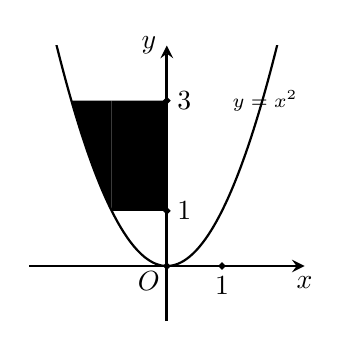
\begin{tikzpicture}[>=stealth, color=black, line width = 1pt, scale=0.7]
		\draw[->] (-5/2,0)--(5/2,0) node[below]{$x$};
		\draw[->](0,-1) -- (0,4) node[left]{$y$};
		\draw(0,0) circle (1pt) node[shift={(220:3mm)}]{$O$};
		\draw(1,0) circle (1pt) node[below]{$1$};
		\draw(0,1) circle (1pt) node[right]{$1$};
		\draw(0,3) circle (1pt) node[right]{$3$};
		\fill(1,3) node[right]{\scriptsize $y=x^2$};
		\clip(-5/2,-1) rectangle (5/2,4);
		\draw[thick,samples=150,smooth,domain=-5/2:5/2] plot(\x,{(\x)^2});
		\fill[black]plot[domain=-1.732:-1](\x,{(\x)^2})--plot[domain=-1:-1.732](\x,{3})--cycle;
		\fill[black]plot[domain=-1:0](\x,{3})--plot[domain=0:-1](\x,{1})--cycle;
		\end{tikzpicture}}
	\loigiai{
		Cách 1: Ta có $\heva{&x^2=3\xrightarrow{{x<0}}x=-\sqrt{3}\\&x^2=1\xrightarrow{{x<0}}x=-1.}$ \\
		Dựa vào đồ thị ta có $S=\displaystyle\int\limits_{-\sqrt{3}}^0\left(3-x^2\right)\mathrm{\,d}x-\displaystyle\int\limits_{-1}^0\left(1-x^2\right)\mathrm{\,d}x =\left(3x-\dfrac{x^3}{3}\right)\bigg|_{-\sqrt{3}}^0-\left(x-\dfrac{x^3}{3}\right)\bigg|_{-1}^0=2\sqrt{3}-\dfrac{2}{3}$.\\
		Cách 2: Do $y=x^2\Rightarrow\hoac{&x=\sqrt{y}\\&x=-\sqrt{y}.}$ \\
		Do trong hình vẽ ta tính phần đồ thị với $x<0$ do đó tính diện tích hình phẳng cần tính là diện tích hình phẳng giới hạn bởi các đường $x=-\sqrt{y}$, $x=0$, $y=1$, $y=3$.\\
		Khi đó $S=\displaystyle\int\limits_1^3\sqrt{y}dy=\dfrac{2}{3}\sqrt{y^3}\bigg|_1^3=2\sqrt{3}-\dfrac{2}{3}$.}
\end{ex}
\begin{ex}%Câu 56.%[2D3B3-1]%[Don Lee]
	\immini
	{Cho hình phẳng $(H)$ giới hạn bởi các đường $y=x^2$, $y=0$, $x=0$, $x=4$. Đường thẳng $y=k,\,\,(0<k<16)$ chia hình $(H)$ thành hai phần có diện tích $S_1$, $S_2$ (hình vẽ). Tìm $k$ để $S_1=S_2$.
		\choice
		{$k=3$}
		{\True $k=4$}
		{$k=5$}
		{$k=8$}}
	{\begin{tikzpicture}[>=stealth, color=black, line width = 1pt, scale=0.6]
		\draw[->] (-5/2,0)--(5/2,0) node[below]{$x$};
		\draw[->](0,-1) -- (0,5) node[left]{$y$};
		\draw(0,0) circle (1pt) node[shift={(220:3mm)}]{$O$};
		\draw[thick] (2,-1)--(2,5)  (-5/2,1)--(5/2,1);
		\fill(-2,4) node[right]{$y=x^2$};
		\fill(5/4,-1) node[right]{$x=4$};
		\fill(-2,1) node[above]{$y=k$};
		\fill(3/2,1/2) node[blue]{$S_1$};
		\fill(5/3,7/4) node[red]{$S_2$};
		\clip(-5/2,-1) rectangle (5/2,5);
		\draw[thick,samples=150,smooth,domain=-5/2:5/2] plot(\x,{(\x)^2});
		\fill[pattern=north west lines]plot[domain=0:1](\x,{(\x)^2})--plot[domain=1:0](\x,{0})--cycle;
		\fill[pattern=north west lines]plot[domain=1:2](\x,{(1})--plot[domain=2:1](\x,{0})--cycle;
		\fill[pattern=north east lines]plot[domain=1:2](\x,{(\x)^2})--plot[domain=2:1](\x,{1})--cycle;
		\end{tikzpicture}}
	\loigiai{
		Phương trình hoành độ giao điểm: $x^2=k\Rightarrow x=\sqrt{k}$.\\
		Ta có\\
		$S_1+S_2=\displaystyle\int\limits_0^4 x^2\mathrm{\,d}x=\dfrac{x^3}{3}\bigg|_0^4=\dfrac{64}{3}$.\\
		$S_1=\displaystyle\int\limits_{\sqrt{k}}^4\left(x^2-k\right)\mathrm{\,d}x=\left(\dfrac{x^3}{3}-kx\right)\bigg|_{\sqrt{k}}^4=-4k+\dfrac{2k\sqrt{k}}{3}+\dfrac{64}{3}$.\\
		Yêu cầu bài toán $\Leftrightarrow S_1=\dfrac{1}{2}(S_1+S_2)\Leftrightarrow-4k+\dfrac{2k\sqrt{k}}{3}+\dfrac{64}{3}=\dfrac{32}{3}$\\
		$\Leftrightarrow 2k\sqrt{k}-12k+32=0\xrightarrow{t=\sqrt{k}(0<t<4)}2t^3-12t^2+32=0\Rightarrow t=2\Rightarrow k=4$.}
\end{ex}
\begin{ex}%Câu 57.%[2D3K3-2]%[Don Lee]
	\immini
	{Một khuôn viên dạng nửa hình tròn có đường kính bằng $4\sqrt{5}(m)$. Trên đó người thiết kế hai phần để tròng hoa và trồng cỏ Nhật Bản. Phần trồng hoa có dạng của một cánh hoa hình parabol có đỉnh trùng với tâm nửa hình tròn và hai đầu mút của cánh hoa nằm trên nửa đường trong (phần tô màu) cách nhau một khoảng bằng $4m$, phần còn lại của khuôn viên (phần không tô màu) dành để trồng cỏ Nhật Bản. Biết các kích thước như hình vẽ và kinh phí để trồng cỏ Nhật Bản là $200\cdot 000$ đồng/1m$^2$. Hỏi cần bao nhiêu tiền để trồng cỏ Nhật Bản trên phần đất đó? (số tiền được làm tròn đến hàng nghìn)
		\choice
		{\True $3.895\cdot 000$ đồng}
		{$1.948\cdot 000$ đồng}
		{$2.388\cdot 000$ đồng}
		{$1.194\cdot 000$ đồng}}
	{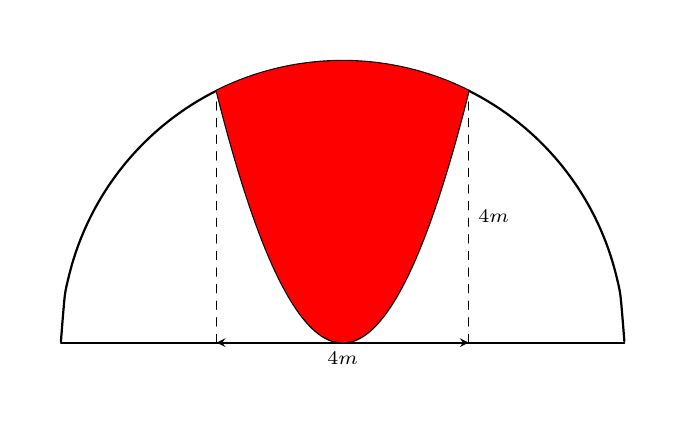
\begin{tikzpicture}[>=stealth,line join=round,line cap=round,font=\footnotesize,scale=0.8]
		\fill (2,2)node[right]{\scriptsize $4m$};
		\fill (0,0)node[below]{\scriptsize $4m$};
		\clip (-5,-1)rectangle(5,5);
		\draw[thick,samples=150,smooth,domain=-2:2] plot(\x,{(\x)^2});
		\draw[thick,samples=150,smooth,domain=-2*sqrt(5):2*sqrt(5)] plot(\x,{sqrt(20-(\x)^2)});
		\draw[dashed] (-2,0)--(-2,4)  (2,0)--(2,4);
		\draw[thick](-4.472136,0)--(4.472136,0);
		\draw[<->] (-2,0)--(2,0);
		\fill[red=north east lines]plot[domain=-2:2](\x,{(\x)^2})--plot[domain=-2:2](\x,{sqrt(20-(\x)^2)})--cycle;
		\end{tikzpicture}}
	\loigiai{
		\immini
		{Gọi $S_1$ là diện tích hình phẳng giới hạn bởi các đường $y=\sqrt{20-x^2}$, $y=x^2$, $x=-2$, $x=2$ được tô màu trong hình bên, $S_2$ là diện tích nửa hình tròn có bán kính bằng $2\sqrt{5}$\\
			Suy ra $S=\dfrac{1}{2}\pi(2\sqrt{5})^2-\displaystyle\int\limits_{-2}^2\left(\sqrt{20-x^2}-x^2\right)\mathrm{\,d}x $.\\
			Vậy $S\approx 19,476(m^2)$ \\
			Do đó chi phí sẽ bằng $200\cdot 000S=3\cdot 895\cdot 000$ đồng.}
		{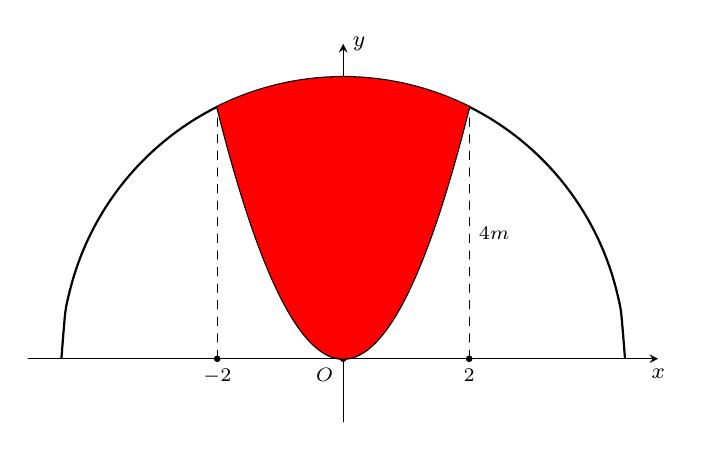
\begin{tikzpicture}[>=stealth,line join=round,line cap=round,font=\footnotesize,scale=0.8]
			\draw[->] (-5,0)--(5,0)node[below]{$x$};
			\draw[->] (0,-1)--(0,5)node[right]{$y$};
			\fill (0,0)node[below left]{\scriptsize $O$}circle(1.5pt);
			\fill (-2,0)node[below]{\scriptsize $-2$}circle(1.5pt);
			\fill (2,0)node[below]{\scriptsize $2$}circle(1.5pt);
			\fill (2,2)node[right]{\scriptsize $4m$};
			\clip (-5,-1)rectangle(5,5);
			\draw[thick,samples=150,smooth,domain=-2:2] plot(\x,{(\x)^2});
			\draw[thick,samples=150,smooth,domain=-2*sqrt(5):2*sqrt(5)] plot(\x,{sqrt(20-(\x)^2)});
			\draw[dashed] (-2,0)--(-2,4)  (2,0)--(2,4);
			\fill[red=north east lines]plot[domain=-2:2](\x,{(\x)^2})--plot[domain=-2:2](\x,{sqrt(20-(\x)^2)})--cycle;
			\end{tikzpicture}}
	}
\end{ex}
\begin{ex}%Câu 58.%[2D3K3-1]%[Don Lee]
	\immini
	{Cho hình thang cong $(H)$ giới hạn bởi các đưởng $y=2^x$, $y=0, x=0, x=4$. Đường thẳng $x=1 (0<a<4)$ chia hình $(H)$ thành hai phần có diện tích là $S_1$ và $S_2$ như hình vẽ bên. Tìm $a$ để $S_2=4S_1$.
		\choice
		{$a=3$}
		{$a=\log_213$}
		{\True $a=2$}
		{$a=\log_2\dfrac{16}{5}$}}
	{\begin{tikzpicture}[>=stealth,line join=round,line cap=round,font=\footnotesize,scale=0.8]
		\draw[->] (-1,0)--(5,0)node[below]{$x$};
		\draw[->] (0,-1/2)--(0,11/2)node[right]{$y$};
		\fill (0,0)node[below left]{\scriptsize $O$}circle(1.5pt);
		\fill (1,0)node[below left]{\scriptsize $a$}circle(1.5pt);
		\fill (4,0)node[below left]{\scriptsize $4$}circle(1.5pt);
		\fill (1/2,1/2)node{\scriptsize $S_1$};
		\fill (5/2,3/2)node{\scriptsize $S_2$};
		\clip (-1,-1/2)rectangle(5,11/2);
		\draw[thick,samples=150,smooth,domain=-1:4.5] plot(\x,{(3/2)^(\x)});
		\draw (1,-1)--(1,11/2)  (4,-1)--(4,11/2);
		\fill[pattern=north east lines]plot[domain=0:1](\x,{(3/2)^(\x)})--plot[domain=1:0](\x,{0})--cycle;
		\fill[pattern=north west lines]plot[domain=1:4](\x,{(3/2)^(\x)})--plot[domain=4:1](\x,{0})--cycle;
		\end{tikzpicture}}
	\loigiai{
		$S_1=\displaystyle\int\limits_0^a 2^x\mathrm{\,d}x=\dfrac{2^x}{\ln 2}\bigg|_0^a=\dfrac{2^a-1}{\ln 2};S_2=\displaystyle\int\limits_a^4 2^x\mathrm{\,d}x=\dfrac{2^x}{\ln 2}\bigg|_a^4=\dfrac{2^4-1}{\ln 2}$.\\
		Từ $S_2=4S_1\Leftrightarrow\dfrac{2^4-2^a}{\ln 2}=4\cdot\dfrac{2^a-1}{\ln 2}\Leftrightarrow 2^a=4\Leftrightarrow a=2$ (thỏa đk).}
\end{ex}
% \begin{ex}%Câu 59.%[2D3K3-2]%[Don Lee]
% 	\immini
% 	{Hình $(H)$ được cho dưới đây là hình phẳng được giới hạn bởi hai đường $(C_1)\colon y=|x|+\sqrt{16-x^2}$, $(C_2)\colon y=|x|-\sqrt{25-x^2}$ và hai đoạn thẳng $(d_1)\colon y=x$ với $x\in[4;5],(d_2)\colon y=-x$ với $x\in[-5;-4]$. Tính diện tích $S$ của hình $(H)$. 
% 		\choice
% 		{$\dfrac{41}{4}$}
% 		{$\dfrac{41\pi}{4}$}
% 		{\True $\dfrac{41\pi}{2}$}
% 		{$\dfrac{41}{2}$}}
% 	{\begin{tikzpicture}[>=stealth,line join=round,line cap=round,font=\footnotesize,scale=0.6]
% 		\fill (0,17/4)node[above]{$(C_1)$};
% 		\fill (-17/4,0)node[above]{$(C_2)$};
% 		\fill (17/4,0)node[above]{$(C_2)$};
% 		\fill (9/2,9/2)node[above]{$d_1$};
% 		\fill (-9/2,9/2)node[above]{$d_2$};
% 		\draw[thick,red,samples=150,smooth,domain=-4:4] plot(\x,{abs(\x)+sqrt(16-(\x)^2)});
% 		\draw[thick,red,samples=150,smooth,domain=-5:5] plot(\x,{abs(\x)-sqrt(25-(\x)^2)});
% 		\draw[thick,red,samples=150,smooth,domain=-5:-4] plot(\x,{-(\x)});
% 		\draw[thick,red,samples=150,smooth,domain=4:5] plot(\x,{(\x)});	
% 		\fill[yellow]plot[domain=-5:-4](\x,{-(\x)})--plot[domain=-4:-5](\x,{abs(\x)-sqrt(25-(\x)^2)})--cycle;
% 		\fill[yellow]plot[domain=-4:4](\x,{abs(\x)+sqrt(16-(\x)^2)})--plot[domain=4:-4](\x,{abs(\x)-sqrt(25-(\x)^2)})--cycle;
% 		\fill[yellow]plot[domain=4:5](\x,{(\x)})--plot[domain=5:4](\x,{abs(\x)-sqrt(25-(\x)^2)})--cycle;
% 		\end{tikzpicture}}
% 	\loigiai{
% 		\immini
% 		{Gọi $S_1$ là diện tích hình phẳng được giới hạn bởi các đường $y=x-\sqrt{25-x^2},y=x,x=0,x=5$ được tô màu trong hình bên suy ra $S_1=\displaystyle\int\limits_0^5\left(x-\left(x-\sqrt{25-x^2}\right)\right)\mathrm{\,d}x=\dfrac{25}{4}\pi$.\\
% 			Gọi S2 là điện tích hình phẳng được giới hạn bởi các đường $y=x+\sqrt{16-x^2},y=x,x=0,x=4$ được tô màu trong hình bên suy ra $S_2=\displaystyle\int\limits_0^4\left(\left(x+\sqrt{16-x^2}\right)-x\right)\mathrm{\,d}x=4\pi$.\\
% 			Diện tích cần tính bằng $S=2(S_1+S_2)=\dfrac{41}{2}\pi$.}
% 		{\begin{tikzpicture}[>=stealth,line join=round,line cap=round,font=\footnotesize,scale=0.6]
% 			\fill (-5,0)node[below]{$-5$}circle(1.0pt);
% 			\fill (-4,0)node[below]{$-4$}circle(1.0pt);
% 			\fill (4,0)node[below]{$4$}circle(1.0pt);
% 			\fill (5,0)node[below]{$5$}circle(1.0pt);
% 			\draw[thick,samples=150,smooth,domain=-4:4] plot(\x,{abs(\x)+sqrt(16-(\x)^2)});
% 			\draw[thick,samples=150,smooth,domain=-5:5] plot(\x,{abs(\x)-sqrt(25-(\x)^2)});
% 			\draw[thick,samples=150,smooth,domain=-5:-4] plot(\x,{-(\x)});
% 			\draw[thick,samples=150,smooth,domain=4:5] plot(\x,{(\x)});	
% 			\fill[yellow]plot[domain=0:5](\x,{(\x)})--plot[domain=5:0](\x,{abs(\x)-sqrt(25-(\x)^2)})--cycle;
% 			\fill[red]plot[domain=0:4](\x,{abs(\x)+sqrt(16-(\x)^2)})--plot[domain=4:0](\x,{(\x)})--cycle;
% 			\draw[->] (-11/2,0)--(11/2,0)node[below]{$x$};
% 			\draw[->] (0,-11/2)--(0,11/2)node[right]{$y$};
% 			\fill (0,0)node[below left]{$O$}circle(1.0pt);
% 			\draw[dashed] (-5,0)--(-5,5)  (-4,0)--(-4,4)  (4,0)--(4,4)  (5,0)--(5,5);
% 			\fill (2,3)node[above]{$(S_2)$};
% 			\fill (2,-1)node[above]{$(S_1)$};
% 			\end{tikzpicture}}
% 	}
% \end{ex}
\Closesolutionfile{ans}
% \DAPAN
\inputansbox{10}{ans/ansCD2D3-3.1.2}
\Opensolutionfile{ans}[ans/ansCD2D3-3.1.3]

\begin{dang}{Ứng dụng tích phân tính diện tích hình phẳng giới hạn bởi $y=f(x),y=g(x)$.}
	\textbf{Phương pháp giải:}\\
	\immini{\textbf{Dạng:} Cho hai hàm số $y=f(x)$ và $y=g(x)$ liên tục trên đoạn $[a; b]$. Diện tích hình phẳng giới hạn bởi các đường $y=f(x)$ và $y=g(x)$ là 
		$$\boxed{S=\displaystyle\int\limits_{\alpha}^{\beta}\left|f(x)-g(x)\right|\mathrm{\,d}x}$$ 
		Trong đó $\alpha,\beta$ là nghiệm nhỏ nhất và lớn nhất của phương trình $f(x)=g(x)\left(a\leq\alpha<\beta\leq b\right)$.
	}{
		\begin{tikzpicture}[>=stealth, color=black, line width = 1pt, scale=.8]
		\draw[->] (0,0)--(5,0) node[above]{$x$};
		\draw[->](0,0) -- (0,5) node[right]{$y$};
		\draw(0,0) circle (1pt) node[below left]{$0$};
		\clip(-1,-1) rectangle (5,5);
		
		\draw[smooth,samples=100,domain=0.7:4.2] 
		plot(\x,{0.333333*(\x)^2-1.333333*(\x)+3.5});
		\draw[smooth,samples=100,domain=0.7:4.2] 
		plot(\x, {-0.25*(\x)^2+1.25*(\x)});
		
		\draw[pattern = north east lines, line width = 1pt,draw=none] (1,2.5)
		plot[domain=1:4] (\x,{0.333333*(\x)^2-1.333333*(\x)+3.5})--(4,3.5)--(4,1)-- plot[domain=4:1] (\x, {-0.25*(\x)^2+1.25*(\x)})--(1,1)--cycle;
		
		\draw(1,0)-- (1,2.5);
		\draw(4,0)-- (4,3.5);
		\begin{scriptsize}
		\draw[color=black] (1,-0.4) node {\normalsize $a$};
		\draw[color=black] (4,-0.4) node {\normalsize $b$};
		\draw[color=black] (2.2,3) node {\normalsize $y=f(x)$};
		\draw[color=black] (2.4,1) node {\normalsize $y=g(x)$};
		\end{scriptsize}
		\end{tikzpicture}
	}
	\textbf{Cách giải:}\\
	Bước 1: Giải phương trình $f(x)=g(x)$ tìm các giá trị $\alpha,\beta$.\\
	Bước 2: Tính $S=\displaystyle\int\limits_{\alpha}^{\beta}\left|f(x)-g(x)\right|\mathrm{\,d}x$. 	\\
	\textbf{Chú ý:} Nếu $f(x)\geq g(x),\forall x\in[a;b]$ thì $S=\displaystyle\int\limits_a^b[f(x)-g(x)]\mathrm{\,d}x$.
\end{dang}
\subsubsection{Các ví dụ}
\begin{vd}%[Nguyễn Tâm Phục]%[2D3B3-1]%Ví dụ 1.
	Diện tích hình phẳng giới hạn bởi các đường $y=x^2$; $y=x+2$ bằng
	\choice
	{$\dfrac{15}{2}$}
	{$\dfrac{-9}{2}$}
	{\True $\dfrac{9}{2}$}
	{$\dfrac{-15}{2}$}
	\loigiai{
		Phương trình hoành độ giao điểm của đồ thị các hàm số là $$x^2=x+2\Leftrightarrow\hoac{&x=-1\\&x=2.}$$
		Do đó diện tích hình phẳng cần tìm là 		
		$$S=\displaystyle\int\limits_{-1}^2\left|x^2-x-2\right|\mathrm{\,d}x=\displaystyle\int\limits_{-1}^2\left(2+x-x^2\right)\mathrm{\,d}x=\dfrac{9}{2}.$$}
\end{vd}
\begin{vd}%[Nguyễn Tâm Phục]%[2D3B3-1]%Ví dụ 2.
	Diện tích hình phẳng giới hạn bởi các đường $y=\left|x^2-4x+3\right|$ và $y=x+3$ bằng 
	\choice
	{$S=\dfrac{106}{6}$}
	{$S=\dfrac{105}{6}$}
	{\True $S=\dfrac{109}{6}$}
	{$S=\dfrac{107}{6}$}
	\loigiai{
		Phương trình hoành độ giao điểm là $$\left|x^2-4x+3\right|=x+3\Leftrightarrow\hoac{&x=0\\&x=5.}$$ 
		Do đó diện tích hình phẳng cần tìm là $$S=\displaystyle\int\limits_0^5\left|\left|x^2-4x+3\right|-x-3\right|\mathrm{\,d}x=\dfrac{109}{6}.$$}
\end{vd}
\begin{vd}%[Nguyễn Tâm Phục]%[2D3K3-1]%Ví dụ 3.
	Diện tích hình phẳng giới hạn bởi parabol $(P)\colon y=x^2-4x+5$ và hai tiếp tuyến của $(P)$ tại các điểm $A(1;2), B(4;5)$ là 
	\choice
	{$\dfrac{13}{4}$}
	{\True $\dfrac{9}{4}$}
	{$\dfrac{15}{4}$}
	{$\dfrac{11}{4}$}
	\loigiai{
		\begin{center}
			\begin{tikzpicture}[line join=round, line cap=round,>=stealth,thick,scale=1]
			\def\xmin{-1}
			\def\xmax{5}
			\def\ymin{-2}
			\def\ymax{6}
			\tikzset{label style/.style={font=\footnotesize}}
			\draw[->] (\xmin,0)--(\xmax,0) node[below left] {$x$};
			\draw[->] (0,\ymin)--(0,\ymax) node[below left] {$y$};
			\draw (0,0) node [below left] {$O$};
			\begin{scope}
			\clip (\xmin,\ymin) rectangle (\xmax,\ymax); 
			\draw[pattern = north east lines, line width = 1.2pt,draw=none](1,2)-- plot[domain=1:2.5] (\x, {-2*(\x)+4})--plot[domain=2.5:4] (\x, {4*(\x)-11})--(4,5);
			\draw[pattern = north east lines, line width = 1.2pt,draw=none,fill=white] plot[domain=0:4] (\x, {(\x)^2-4*(\x)+5})--cycle;		
			
			\draw[samples=200,domain=\xmin:\xmax,smooth,variable=\x] plot (\x,{(\x)^2-4*(\x)+5});
			\draw[samples=200,domain=\xmin:\xmax,smooth,variable=\x] plot (\x,{-2*(\x)+4});
			\draw[samples=200,domain=\xmin:\xmax,smooth,variable=\x] plot (\x,{4*(\x)-11});
			\tkzDrawPoint[fill=black,size=2pt](1,0);
			\tkzLabelPoint[below](1,0){$1$};		
			\draw [dashed](1,0) -- (1,2);
			\tkzDrawPoint[fill=black,size=2pt](2.5,-1);
			\tkzDrawPoint[fill=black,size=2pt](2.5,0);
			\tkzLabelPoint[above,fill=white](2.5,0){$\frac{5}{2}$};
			\draw [dashed](2.5,-1) -- (2.5,0);
			\tkzDrawPoint[fill=black,size=2pt](4,5);
			\tkzLabelPoint[below](4,0){$4$};
			\draw [dashed](4,0) -- (4,5);		
			\end{scope}
			\tkzLabelPoint[left](-0.5,5){$y=-2x+4$};
			\tkzLabelPoint[left](2.25,-2.01){$y=4x-11$};
			\tkzLabelPoint[right](0.44,3.45){$y=x^2-4x+5$};
			\end{tikzpicture}
		\end{center}
		\begin{itemize}
			\item Phương trình tiếp tuyến với $(P)$ tại $A(1;2)$ là $y=-2x+4$.
			\item Phương trình tiếp tuyến với $(P)$ tại $B(4;5)$ là $y=4x-11$.
			\item Giao của hai tiếp tuyến có hoành độ $x=\dfrac{5}{2}$.
			\item Xét phương trình $x^2-4x+5=-2x+4\Leftrightarrow x=1$.
			\item Xét phương trình $x^2-4x+5=4x-11\Leftrightarrow x=4$.
			\item Do đó diện tích hình phẳng cần tìm là $$S=\displaystyle\int\limits_1^{\tfrac{5}{2}}\left|x^2-4x+5+2x-4\right|\mathrm{\,d}x+\displaystyle\int\limits_{\tfrac{5}{2}}^4\left|x^2-4x+5-4x+11\right|\mathrm{\,d}x=\dfrac{9}{4}.$$
		\end{itemize}
	}
\end{vd}
\begin{vd}%[Nguyễn Tâm Phục]%[2D3G3-1]%Ví dụ 4.
	\immini{Cho parabol $(P)\colon y=-x^2+2x$, có đỉnh $S$ và $A$ là giao điểm khác $O$ của $(P)$ và trục hoành. $M$ là điểm di động trên đường cong $SA$ của $(P)$, tiếp tuyến của $(P)$ tại $M$ cắt $Ox,Oy$ lần lượt tại $E$ và $F$. Tìm giá trị nhỏ nhất của tổng diện tích $2$ tam giác cong $MOE$ và $MAF$ thì giá trị của m là 
		\choice
		{$\dfrac{5}{3}$}
		{$4$}
		{\True $\dfrac{4}{3}$}
		{$13$}
	}{
		\begin{tikzpicture}[line join=round, line cap=round,>=stealth,thick,scale=1]
		\def\xmin{-1}
		\def\xmax{4}
		\def\ymin{-1}
		\def\ymax{3}
		\tikzset{label style/.style={font=\footnotesize}}
		\draw[->] (\xmin,0)--(\xmax,0) node[below left] {$x$};
		\draw[->] (0,\ymin)--(0,\ymax) node[below left] {$y$};
		\draw (0,0) node [below left] {$O$};
		\begin{scope}
		
		\clip (\xmin,\ymin) rectangle (\xmax,\ymax); 
		\draw[pattern = north east lines, line width = 1.2pt,draw=none](0,0)--(0,2)--plot[domain=0:2.25] (\x, {-(\x)+2.25})--cycle;
		\draw[pattern = north east lines, line width = 1.2pt,draw=none,fill=white](0,0)--(0,2)--plot[domain=0:2] (\x, {-(\x)^2+2*(\x)})--cycle;
		\draw[samples=200,domain=\xmin:\xmax,smooth,variable=\x] plot (\x,{-(\x)^2+2*(\x)});
		\draw[samples=200,domain=\xmin:\xmax,smooth,variable=\x] plot (\x,{-(\x)+2.25});
		\tkzDrawPoint[fill=black,size=2pt](1,1);\tkzLabelPoint[below left](1,1){$S$};
		\tkzDrawPoint[fill=black,size=2pt](2,0);
		\tkzLabelPoint[below left](2,0){$2$};
		\tkzLabelPoint[above left](2,-0.1){$A$};
		\tkzDrawPoint[fill=black,size=2pt](0,2.25);
		\tkzLabelPoint[left](0,2.25){$E$};
		\tkzDrawPoint[fill=black,size=2pt](2.25,0);
		\tkzLabelPoint[above right](2.25,0){$F$};
		\tkzDrawPoint[fill=black,size=2pt](1.5,0.75);
		\tkzLabelPoint[right](1.5,0.75){$M$};
		\tkzDrawPoint[fill=black,size=2pt](0,1);
		\tkzDrawPoint[fill=black,size=2pt](1,0);
		\tkzLabelPoint[left](0,1){$1$};
		\tkzLabelPoint[below](1,0){$1$};
		\draw [dashed](1,0) -- (1,1)--(0,1);
		\end{scope}
		\end{tikzpicture}
	}
	\loigiai{	
		Tiếp tuyến tại $M\left(m;2m-m^2\right),1\leq m\leq 2$ có phương trình 
		$$y=(2-2m)(x-m)+2m-m^2\Leftrightarrow y=(2-2m)x+m^2.$$
		Ta có: $E\left(0;m^2\right);F\left(\dfrac{m^2}{2m-2};0\right)$ với $1<m\leq 2$.\\
		Gọi $S$ là diện tích hình phẳng giới hạn bởi $(P)$ và trục hoành. Khi đó $$S=\displaystyle\int\limits_0^2\left|-x^2+2x\right|\mathrm{\,d}x=\dfrac{4}{3}.$$ 
		Lại có
		$$S_{OEF}=\dfrac{1}{2}\left|\dfrac{m^4}{2m-2}\right|=\dfrac{m^4}{4(m-1)}.$$
		Ta thấy, $S_{MOE}+S_{MAF}=S_{OEF}-S,\left(S_{MOE}+S_{MAF}\right)\min\Leftrightarrow(S_{OEF})\min$.\\
		$\left(S_{MOE}+S_{MAF}\right)\min=\left(\dfrac{4}{3}\right)^3-\dfrac{4}{3}=\dfrac{28}{27}$ khi $m=\dfrac{4}{3}$.\\
		Vậy $m=\dfrac{4}{3}$ thỏa bài toán.
	}
\end{vd}
\subsubsection{Câu hỏi trắc nghiệm}
\begin{ex}%[Nguyễn Tâm Phục]%[2D3B3-1]%Câu 60.
	Diện tích hình phẳng giới hạn bởi các đường $y=x+3, y=x^2-4x+3$ là 
	\choice
	{$\dfrac{25}{6}$}
	{\True $\dfrac{125}{6}$}
	{$\dfrac{625}{6}$}
	{$\dfrac{124}{6}$}
	\loigiai{
		Phương trình hoành độ giao điểm của hai đường đã cho là $$x+3=x^2-4x+3\Leftrightarrow x^2-5x=0\Leftrightarrow\hoac{&x=0\\&x=5.}$$ 
		Do đó diện tích hình phẳng cần tìm là $$S=\displaystyle\int\limits_0^5\left|x^2-5x\right|\mathrm{\,d}x=\left(\dfrac{x^3}{3}-5\cdot\dfrac{x^2}{2}\right)\bigg|_0^5=\dfrac{125}{6}.$$}
\end{ex}
\begin{ex}%[Nguyễn Tâm Phục]%[2D3B3-1]%Câu 61.
	Diện tích hình phẳng giới hạn bởi đồ thị hai hàm số $y=x^3, y=4x$ là 
	\choice
	{\True $8$}
	{$9$}
	{$12$}
	{$13$}
	\loigiai{
		Phương trình hoành độ giao điểm của đồ thị hai hàm số là $$x^3=4x\Leftrightarrow \hoac{&x=-2\\&x=0\\&x=2.}$$
		Suy ra diện tích hình phẳng cần tìm là $$S=\left|\displaystyle\int\limits_{-2}^{0}\left(x^3-4x\right)\mathrm{\,d}x\right|+\left|\displaystyle\int\limits_0^2\left(x^3-4x\right)\mathrm{\,d}x\right|=8.$$
		\textbf{Lưu ý: }Nếu trong đoạn $\left[\alpha;\beta\right]$ phương trình $f(x)=g(x)$ không còn nghiệm nào nữa thì ta có thể dùng công thức $$S=\displaystyle\int\limits_{\alpha}^{\beta}\left|f(x)-g(x)\right|\mathrm{\,d}x=\left|\displaystyle\int\limits_{\alpha}^{\beta}[f(x)-g(x)]\mathrm{\,d}x\right|.$$}
\end{ex}
\begin{ex}%[Nguyễn Tâm Phục]%[2D3B3-1]%Câu 62.
	Diện tích hình phẳng được giới hạn bởi parabol $y=2-x^2$ và đường thẳng $y=-x$ là 
	\choice
	{\True $\dfrac{9}{2}$}
	{$\dfrac{9}{4}$}
	{$3$}
	{$\dfrac{7}{2}$}
	\loigiai{
		Phương trình hoành độ giao điểm của đồ thị hai hàm số là $$2-x^2=-x\Leftrightarrow\hoac{&x=-1\\&x=2.}$$
		Do đó diện tích hình phẳng cần tìm là $$S=\displaystyle\int\limits_{-1}^2\left|2+x-x^2\right|\mathrm{\,d}x=\displaystyle\int\limits_{-1}^2\left(2+x-x^2\right)\mathrm{\,d}x=\dfrac{9}{2}.$$}
\end{ex}
\begin{ex}%[Nguyễn Tâm Phục]%[2D3B3-1]%Câu 63.
	Diện tích hình phẳng giới hạn bởi đồ thị hai hàm số $y=\sqrt{x}$ và $y=\sqrt[3]{x}$ là 
	\choice
	{$\dfrac{1}{15}$}
	{$\dfrac{1}{13}$}
	{$\dfrac{1}{14}$}
	{\True $\dfrac{1}{12}$}
	\loigiai{
		Phương trình hoành độ giao điểm của đồ thị hai hàm số là  $$\sqrt{x}=\sqrt[3]{x}\Leftrightarrow\hoac{&x=0\\&x=1.}$$
		Do đó diện tích hình phẳng cần tìm là $$S=\displaystyle\int\limits_0^1\left|\sqrt{x}-\sqrt[3]{x}\right|\mathrm{\,d}x=\dfrac{1}{12}.$$}
\end{ex}
\begin{ex}%[Nguyễn Tâm Phục]%[2D3B3-1]%Câu 64.
	Diện tích hình phẳng giới hạn bởi các đường $y=x^3-12x$ và $y=x^2$ là 
	\choice
	{$\dfrac{210}{12}$}
	{$\dfrac{56}{12}$}
	{\True $\dfrac{937}{12}$}
	{$12$}
	\loigiai{
		Phương trình hoành độ giao điểm của đồ thị hai hàm số là $$x^3-12x=x^2\Leftrightarrow\hoac{&x=0\\&x=-3\\&x=4.}$$
		Do đó diện tích hình phẳng cần tìm là 
		\begin{eqnarray*}
			&S&=\displaystyle\int\limits_{-3}^4\left|x^3-12x-x^2\right|\mathrm{\,d}x=\displaystyle\int\limits_{-3}^{0}\left|x^3-12x-x^2\right|\mathrm{\,d}x+\displaystyle\int\limits_0^4\left|x^3-12x-x^2\right|\mathrm{\,d}x\\
			&&=\left|\displaystyle\int\limits_{-3}^{0}\left(x^3-12x-x^2\right)\mathrm{\,d}x\right|+\left|\displaystyle\int\limits_0^4\left(x^3-12x-x^2\right)\mathrm{\,d}x\right|=\dfrac{937}{12}.
		\end{eqnarray*}
	}
\end{ex}
\begin{ex}%[Nguyễn Tâm Phục]%[2D3B3-1]%Câu 65.
	Diện tích hình phẳng giới hạn bởi các đường $y=x^2+x-1, y=x^4+x-1$ là 
	\choice
	{$\dfrac{8}{15}$}
	{$\dfrac{7}{15}$}
	{$-\dfrac{7}{15}$}
	{\True $\dfrac{4}{15}$}
	\loigiai{
		Phương trình hoành độ giao điểm của các đường là $$x^2+x-1=x^4+x-1\Leftrightarrow x^4-x^2=0\Leftrightarrow\hoac{&x=0\\&x=1\\&x=-1.}$$
		Do đó diện tích hình phẳng cần tìm là $$S=\displaystyle\int\limits_{-1}^1\left|x^4-x^2\right|\mathrm{\,d}x=\left|2\displaystyle\int\limits_0^1\left(x^4-x^2\right)\mathrm{\,d}x\right|=\left|2\left(\dfrac{x^5}{5}-\dfrac{x^3}{3}\right)\bigg|_0^1\right|=\dfrac{4}{15}.$$}
\end{ex}
\begin{ex}%[Nguyễn Tâm Phục]%[2D3B3-1]%Câu 66.
	Diện tích hình phẳng giới hạn bởi các đường $y=x^2, y=\sqrt{x}$ là 
	\choice
	{$\dfrac{2}{3}$}
	{$\dfrac{4}{3}$}
	{$\dfrac{5}{3}$}
	{\True $\dfrac{1}{3}$}
	\loigiai{
		Phương trình hoành độ giao điểm của đồ thị các hàm số là $$x^2=\sqrt{x}\Leftrightarrow\hoac{&x=0\\&x=1.}$$ 
		Do đó diện tích hình phẳng cần tìm là $$S=\displaystyle\int\limits_0^1\left|x^2-\sqrt{x}\right|\mathrm{\,d}x=\left|\displaystyle\int\limits_0^1\left(x^2-\sqrt{x}\right)\mathrm{\,d}x\right|=\left|\left(\dfrac{x^3}{3}-\dfrac{2}{3}x^{\tfrac{3}{2}}\right)\bigg|_0^1\right|=\dfrac{1}{3}.$$}
\end{ex}
\begin{ex}%[Nguyễn Tâm Phục]%[2D3B3-1]%Câu 67.
	Diện tích hình phẳng giới hạn bởi đồ thị hai hàm số $y=2x^3-3x^2+1$ và $y=x^3-4x^2+2x+1$ là 
	\choice
	{$\dfrac{37}{13}$}
	{\True $\dfrac{37}{12}$}
	{$3$}
	{$4$}
	\loigiai{
		Phương trình hoành độ giao điểm của đồ thị hai hàm số là $$2x^3-3x^2+1=x^3-4x^2+2x+1\Leftrightarrow\hoac{&x=-2\\&x=0\\&x=1.}$$
		Do đó diện tích hình phẳng cần tìm là 
		\begin{eqnarray*}
			&S&=\displaystyle\int\limits_{-2}^1\left|x^3+x^2-2x\right|\mathrm{\,d}x=\left|\displaystyle\int\limits_{-2}^{0}\left(x^3+x^2-2x\right)\right|+\left|\displaystyle\int\limits_0^1\left(x^3+x^2-2x\right)\right|.\\
			&&=\left|\left(\dfrac{x^4}{4}+\dfrac{x^3}{3}-x^2\right)\bigg|_{-2}^{0}\right|+\left|\left(\dfrac{x^4}{4}+\dfrac{x^3}{3}-x^2\right)\bigg|_0^1\right|=\dfrac{37}{12}.
		\end{eqnarray*}	
	}
\end{ex}
\begin{ex}%[Nguyễn Tâm Phục]%[2D3B3-1]%Câu 68.
	Cho S là diện tích hình phẳng giới hạn bởi đồ thị hàm số $y=x^3-6x^2+9x$ và trục $Ox$. Số nguyên lớn nhất không vượt quá S là 
	\choice
	{$10$}
	{\True $6$}
	{$8$}
	{$4$}
	\loigiai{
		Phương trình hoành độ giao điểm của đồ thị  hàm số và trục hoành là $$x^3-6x^2+9x=0\Leftrightarrow\hoac{&x=0\\&x=3.}$$
		Do đó diện tích hình phẳng cần tìm là $$S=\displaystyle\int\limits_0^3\left|x^3-6x^2+9x\right|\mathrm{\,d}x=\displaystyle\int\limits_0^3\left(x^3-6x^2+9x\right)\mathrm{\,d}x=\left(\dfrac{x^4}{4}-2x^3+\dfrac{9}{2}x^2\right)\bigg|_0^3=\dfrac{27}{4}.$$}
\end{ex}
\begin{ex}%[Nguyễn Tâm Phục]%[2D3B3-1]%Câu 69.
	Diện tích hình phẳng giới hạn bởi các đường $y=-1, y=x^4-2x^2-1$ là 
	\choice
	{$\dfrac{6\sqrt{2}}{5}$}
	{$\dfrac{28}{3}$}
	{\True $\dfrac{16\sqrt{2}}{15}$}
	{$\dfrac{27}{4}$}
	\loigiai{
		Phương trình hoành độ giao điểm của các đường là  $$-1=x^4-2x^2-1\Leftrightarrow x^4-2x^2=0\Leftrightarrow\hoac{&x=0\\&x=\sqrt{2}\\&x=-\sqrt{2}.}$$
		Do đó diện tích hình phẳng cần tìm là 
		$$S=\displaystyle\int\limits_{-\sqrt{2}}^{\sqrt{2}}\left|x^4-2x^2\right|\mathrm{\,d}x=\dfrac{16\sqrt{2}}{15}.$$}
\end{ex}
\begin{ex}%[Nguyễn Tâm Phục]%[2D3B3-1]%Câu 70.
	Diện tích hình phẳng giới hạn bởi các đường $y=\dfrac{x^3}{1-x^2}, y=x$ là 
	\choice
	{$1$}
	{\True $1-\ln 2$}
	{$1+\ln 2$}
	{$2-\ln 2$}
	\loigiai{
		Phương trình hoành độ giao điểm của đồ thị các hàm số là $$\dfrac{x^3}{1-x^2}=x\Leftrightarrow x^3=x-x^3\Leftrightarrow 2x^3-x=0\Leftrightarrow\hoac{&x=0\\&x=\dfrac{1}{\sqrt{2}}\\&x=-\dfrac{1}{\sqrt{2}}.}$$
		Do đó diện tích hình phẳng cần tìm là $$S=\displaystyle\int\limits_{-\tfrac{1}{\sqrt{2}}}^{\tfrac{1}{\sqrt{2}}}\left|\dfrac{x^3}{1-x^2}-x\right|\mathrm{\,d}x=\displaystyle\int\limits_{-\tfrac{1}{\sqrt{2}}}^{0}\left|\dfrac{x^3}{1-x^2}-x\right|\mathrm{\,d}x+\displaystyle\int\limits_0^{\tfrac{1}{\sqrt{2}}}\left|\dfrac{x^3}{1-x^2}-x\right|\mathrm{\,d}x=1-\ln 2 .$$}
\end{ex}
\begin{ex}%[Nguyễn Tâm Phục]%[2D3K3-1]%Câu 71.
	Gọi $(H)$ là diện tích hình phẳng được giới hạn bởi đồ thị hai hàm số $y=\left(1+\mathrm{e}^x\right)x$, $y=(1+e)x$. Diện tích của $(H)$ bằng
	\choice
	{$\dfrac{e+2}{2}$}
	{$\dfrac{e-1}{2}$}
	{\True $\dfrac{e-2}{2}$}
	{$\dfrac{e+1}{2}$}
	\loigiai{
		Phương trình hoành độ giao điểm của đồ thị các hàm số là $$\left(1+\mathrm{e}^x\right)x-(1+e)x=0 \Leftrightarrow x(\mathrm{e}^x-e)=0\Leftrightarrow\hoac{&x=0\\&x=1.}$$
		Do đó diện tích hình phẳng cần tìm là $$S=\displaystyle\int\limits_0^1\left|x\left(e-\mathrm{e}^x\right)\right|\mathrm{\,d}x=\displaystyle\int\limits_0^1 x\left(e-\mathrm{e}^x\right)\mathrm{\,d}x=\dfrac{e-2}{2} .$$}
\end{ex}
\begin{ex}%[Nguyễn Tâm Phục]%[2D3K3-1]%Câu 72.
	Diện tích hình phẳng giới hạn bởi các đường $y^2=2x, y=2x-2$ là 
	\choice
	{$\dfrac{5}{4}$}
	{\True $\dfrac{9}{4}$}
	{$\dfrac{11}{2}$}
	{$3$}
	\loigiai{
		\begin{center}
			\begin{tikzpicture}[line join=round, line cap=round,>=stealth,thick,scale=1]
			\def\xmin{-1}
			\def\xmax{3.5}
			\def\ymin{-4}
			\def\ymax{4}
			\tikzset{label style/.style={font=\footnotesize}}
			\draw[->] (\xmin,0)--(\xmax,0) node[below left] {$x$};
			\draw[->] (0,\ymin)--(0,\ymax) node[below left] {$y$};
			\draw (0,0) node [below left] {$O$};
			\begin{scope}
			\clip (\xmin,\ymin) rectangle (\xmax,\ymax); 
			\draw[samples=200,domain=0:\xmax,smooth,variable=\x] plot (\x,{sqrt(2*\x)});
			\draw[samples=200,domain=0:\xmax,smooth,variable=\x] plot (\x,-{sqrt(2*\x)});
			\draw[samples=200,domain=\xmin:\xmax,smooth,variable=\x] plot (\x,{2*(\x)-2});
			\draw[pattern = north east lines, line width = 1.2pt,draw=none]plot[domain=0:0.5] (\x, {sqrt(2*(\x))})--(0.5,0);
			\draw[pattern = north east lines, line width = 1.2pt,draw=none]plot[domain=0:0.5] (\x, {-sqrt(2*(\x))})--(0.5,0);
			\draw[pattern = north west lines, line width = 1.2pt,draw=none](0.5,-1)--plot[domain=0.5:2] (\x, {sqrt(2*(\x))})--plot[domain=0.5:2] (\x, {2*(\x)-2})--(1,0);
			\draw (0.5,-1) -- (0.5,1);
			\tkzLabelPoint[right](2,1.7){$y^2=2x$};
			\tkzLabelPoint[left](2.64,3.22){$y=2x-2$};
			\tkzLabelPoint[above right,fill=white](0.5,0){$\frac{1}{2}$};
			\draw [dashed](2,0) -- (2,2);
			\tkzLabelPoint[below](2,0){$2$};
			\tkzDrawPoint[fill=black,size=2pt](2,0);
			\end{scope}
			\end{tikzpicture}
		\end{center}
		Phương trình hoành độ giao điểm của đồ thị các hàm số là $$(2x-2)^2=2x\Leftrightarrow 2x^2-5x+2=0\Leftrightarrow\hoac{&x=2\\&x=\dfrac{1}{2}.}$$
		Do đó, diện tích hình phẳng cần tìm là $$S=2\displaystyle\int\limits_0^{\tfrac{1}{2}}\sqrt{2x}\mathrm{\,d}x+\displaystyle\int\limits_{\tfrac{1}{2}}^2\left[\sqrt{2x}-2x+2\right]\mathrm{\,d}x=\dfrac{4\sqrt{2}}{3}\sqrt[3]{x}\bigg|_0^{\tfrac{1}{2}}+\left(\dfrac{2\sqrt{2}}{3}\sqrt{x^3}-x^2+2x\right)\bigg|_{\tfrac{1}{2}}^2=\dfrac{9}{4}.$$}
\end{ex}
\begin{ex}%[Nguyễn Tâm Phục]%[2D3B3-1]%Câu 73.
	Diện tích hình phẳng giới hạn bởi các đường $y=x, y=\sin^2x+x$, $(0<x<\pi)$ là 
	\choice
	{$\pi$}
	{\True $\dfrac{\pi}{2}$}
	{$2\pi$}
	{$\dfrac{\pi}{3}$}
	\loigiai{
		Phương trình hoành độ giao điểm của các đường đã cho là $$x+\sin^2x=x\Leftrightarrow\sin^2x=0\Leftrightarrow\hoac{&x=0\\&x=\pi.}$$ \\
		Do đó, diện tích hình phẳng cần tìm là $$S=\displaystyle\int\limits_0^{\pi}\left|\sin^2x\right|\mathrm{\,d}x=\left (\dfrac{1}{2}x -\dfrac{\sin 2x}{4}\right )\bigg|_0^{\pi}=\dfrac{1}{2}\pi$$.}
\end{ex}
\begin{ex}%[Nguyễn Tâm Phục]%[2D3K3-1]%Câu 74.
	Diện tích hình phẳng giới hạn bởi các đường $y=|\ln x|; y=1$ là 
	\choice
	{$\mathrm{e}-2\mathrm{e}^2+2$}
	{\True $\mathrm{e}-\dfrac{3}{\mathrm{e}}+2$}
	{$\mathrm{e}^2+2\mathrm{e}-1$}
	{3}
	\loigiai{
		Phương trình hoành độ giao điểm của đồ thị các hàm số là $$|\ln x|=1\Rightarrow\hoac{&x=\mathrm{e}\\&x=\dfrac{1}{\mathrm{e}}.}$$ 
		Do đó, diện tích hình phẳng cần tìm là $$S=\displaystyle\int\limits_{\tfrac{1}{e}}^e\left||\ln x|-1\right|\mathrm{\,d}x=\displaystyle\int\limits_{\tfrac{1}{e}}^{0} (1+\ln x)\mathrm{\,d}x+\displaystyle\int\limits_0^e (\ln x-1)\mathrm{\,d}x=\mathrm{e}-\dfrac{3}{\mathrm{e}}+2.$$}
\end{ex}
\begin{ex}%[Nguyễn Tâm Phục]%[2D3B3-1]%Câu 75.
	Diện tích hình phẳng giới hạn bởi các đường $y=x+\sin x, y=x\left(0\leq x\leq\pi\right)$ là 
	\choice
	{$1$}
	{\True $2$}
	{$3$}
	{$4$}
	\loigiai{
		Phương trình hoành độ giao điểm của các đường là $$x+\sin x=x\Leftrightarrow\sin x=0\Leftrightarrow\hoac{&x=0\\&x=\pi.}$$ \\
		Do đó, diện tích hình phẳng cần tìm là $$S=\displaystyle\int\limits_0^{\pi}\left|\sin x\right|\mathrm{\,d}x=\displaystyle\int\limits_{0}^{\pi}\sin x\mathrm{\,d}x= -\cos x\bigg|_0^{\pi}=2.$$}
\end{ex}
\begin{ex}%[Nguyễn Tâm Phục]%[2D3K3-1]%Câu 76.
	Diện tích hình phẳng giới hạn bởi $(P)\colon y=x^2+3$, tiếp tuyến của $(P)$ tại điểm có hoành độ $x=2$ và trục tung bằng
	\choice
	{$\dfrac{17}{3}$}
	{\True $\dfrac{8}{3}$}
	{$2$}
	{$\dfrac{7}{3}$}
	\loigiai{
		Phương trình tiếp tuyến của $(P)$ tại $x=2$ là $y=4x+3$.\\
		Phương trình hoành độ giao điểm của $(P)$ và tiếp tuyến là $$(x^2+3)-(4x+3)=0 \Leftrightarrow x^2-4x=0\Leftrightarrow\hoac{&x=0\\&x=2.}$$ 
		Do đó, diện tích hình phẳng cần tìm là $$S=\displaystyle\int\limits_0^2\left|\left(x^2-4x+4\right)\right|\mathrm{\,d}x=\left|\displaystyle\int\limits_0^2\left(x^2-4x+4\right)\mathrm{\,d}x\right|=\left|\left(\dfrac{x^3}{3}-2x^2+4x\right)\bigg|_0^2\right|=\dfrac{8}{3}.$$}
\end{ex}
\begin{ex}%[Nguyễn Tâm Phục]%[2D3K3-1]%Câu 77.
	Diện tích hình phẳng giới hạn bởi hai đường $x=-2y^2$ và $x=1-3y^2$ được viết dưới dạng $\dfrac{a}{b}$. Khi đó $a$ và $b$ là nghiệm của phương trình
	\choice
	{$x^2-4x+3=0$}
	{$x^2-6x+8=0$}
	{\True $x^2-7x+12=0$}
	{$x^2-5x+6=0$}
	\loigiai{
		Phương trình tung độ giao điểm của hai đường đã cho là $$-2y^2=1-3y^2\Leftrightarrow y^2=1\Leftrightarrow\hoac{&y=1\\&y=-1.}$$\
		Do đó, diện tích hình phẳng cần tìm là $S=\displaystyle\int\limits_{-1}^1\left|y^2-1\right|\mathrm{\,d}y=2\left(y-\dfrac{y^3}{3}\right)\bigg|_0^1=\dfrac{4}{3}$.\\
		Suy ra $a=4, b=3$.\\
		Vậy $a,b$ là nghiệm của phương trình $x^2-7x+12=0$.}
\end{ex}
\begin{ex}%[Nguyễn Tâm Phục]%[2D3K3-1]%Câu 78.
	Diện tích hình phẳng giới hạn bởi đồ thị hai hàm số $y^2-2y+x=0$, $x+y=0$ là 
	\choice
	{$\dfrac{109}{6}$}
	{$\dfrac{109}{5}$}
	{$\dfrac{108}{5}$}
	{\True $\dfrac{9}{2}$}
	\loigiai{
		Biến đổi về hàm số theo biến số $y$ là $x=-y^2+2y, x=-y$.\\
		Phương trình tung độ giao điểm của đồ thị hai hàm số là $$-y^2+2y-(-y)=0\Leftrightarrow\hoac{&y=0\\&y=3.}$$ 
		Do đó diện tích hình phẳng cần tìm là $$S=\displaystyle\int\limits_0^3\left|-y^2+3y\right|dy=\displaystyle\int\limits_0^3\left(-y^2+3y\right)dy=\dfrac{9}{2}.$$}
\end{ex}
\begin{ex}%[Nguyễn Tâm Phục]%[2D3K3-1]%Câu 79.
	Diện tích hình phẳng giới hạn bởi hai đồ thị hàm số $y=ax^3$, $(a>0),$ trục hoành và hai đường thẳng $x=-1,x=k$, $(k>0)$ bằng $\dfrac{17a}{4}$. Tìm $k$. 
	\choice
	{$k=1$}
	{$k=\dfrac{1}{4}$}
	{$k=\dfrac{1}{2}$}
	{\True $k=2$}
	\loigiai{
		Ta có: $I=\displaystyle\int\limits_{-1}^k\left|ax^3\right|\mathrm{\,d}x=a\left(\displaystyle\int\limits_{-1}^{0}-x^3\mathrm{\,d}x+\displaystyle\int\limits_0^k x^3\mathrm{\,d}x\right)=a\left(\dfrac{1}{4}+\dfrac{k^4}{4}\right)=\dfrac{17a}{4}\Rightarrow k=2$.}
\end{ex}
\begin{ex}%[Nguyễn Tâm Phục]%[2D3K3-1]%Câu 80.
	Tính diện tích  hình phẳng được giới hạn bởi các đường $y=\left|x^2-4\right|,y=\dfrac{x^2}{2}+4$. 
	\choice
	{\True $S=\dfrac{64}{3}$}
	{$S=\dfrac{32}{3}$}
	{$S=8$}
	{$S=16$}
	\loigiai{
		Phương trình hoành độ giao điểm của đồ thị các hàm số là $$\left|x^2-4\right|=\dfrac{x^2}{2}+4\Leftrightarrow\hoac{&x^2-4=\dfrac{x^2}{2}+4,\left(x\leq-2\vee x\geq 2\right)\\&4-x^2=\dfrac{x^2}{2}+4,(-2<x<2)}\Leftrightarrow\hoac{&x=\pm 4\\&x=0.}$$ 
		Do đó, diện tích hình phẳng cần tìm là $$S=\displaystyle\int\limits_{-4}^4\left|\left|x^2+4\right|-\left(\dfrac{x^2}{2}+4\right)\right|\mathrm{\,d}x=\dfrac{64}{3}.$$}
\end{ex}
\begin{ex}%[Nguyễn Tâm Phục]%[2D3K3-1]%Câu 81.
	Hình phẳng $(H)$ được giới hạn bởi đồ thị hai hàm số $y=\left|x^2-1\right|$ và $y=|x|+5$. Diện tích của $(H)$ bằng 
	\choice
	{$\dfrac{74}{3}$}
	{$\dfrac{71}{3}$}
	{$\dfrac{70}{3}$}
	{\True $\dfrac{73}{3}$}
	\loigiai{
		Phương trình hoành độ giao điểm của đồ thị các hàm số là $$\left|x^2-1\right|=|x|+5\Leftrightarrow\hoac{&x=-3\\&x=3.}$$
		Do đó, diện tích hình phẳng cần tìm là 
		$$\begin{aligned}&S=\displaystyle\int\limits_{-3}^3\left|\left(\left|x^2-1\right|-(|x|+5)\right)\right|\mathrm{\,d}x=2\displaystyle\int\limits_0^3\left|\left(\left|x^2-1\right|-(|x|+5)\right)\right|\mathrm{\,d}x\\&=2\left|\displaystyle\int\limits_0^1\left(-x^2-x-4\right)\mathrm{\,d}x+\displaystyle\int\limits_1^3\left(x^2-x-6\right)\mathrm{\,d}x\right|=\dfrac{73}{3}\end{aligned}.$$}
\end{ex}
\begin{ex}%[Nguyễn Tâm Phục]%[2D3K3-1]%Câu 82.
	Diện tích hình phẳng giới hạn bởi các đường $y=\sqrt{4-\dfrac{x^2}{4}}$ và $y=\dfrac{x^2}{4\sqrt{2}}$ là 
	\choice
	{$\dfrac{4}{3}$}
	{$2\pi$}
	{$2\pi-\dfrac{4}{3}$}
	{\True $2\pi+\dfrac{4}{3}$}
	\loigiai{
		\begin{center}
			\begin{tikzpicture}[line join=round, line cap=round,>=stealth,thick,scale=1]
			\def\xmin{-5}
			\def\xmax{5}
			\def\ymin{-1}
			\def\ymax{3}
			\tikzset{label style/.style={font=\footnotesize}}
			\draw[->] (\xmin,0)--(\xmax,0) node[below left] {$x$};
			\draw[->] (0,\ymin)--(0,\ymax) node[below left] {$y$};
			\draw (0,0) node [below left] {$O$};
			\begin{scope}
			\clip (\xmin,\ymin) rectangle (\xmax,\ymax); 
			\draw[samples=200,domain=-4:4,smooth,variable=\x] plot (\x,{sqrt(4-(\x)^2/4)});
			\draw[samples=200,domain=\xmin:\xmax,smooth,variable=\x] plot (\x,{((\x)^2)/(5.66)});
			\draw[pattern = north east lines, line width = 1.2pt,draw=none] plot[domain=-2.83:2.83] (\x, {((\x)^2)/(5.66)})--plot[domain=-2.83:2.83] (\x, {sqrt(4-(\x)^2/4)});
			\draw [dashed](-2.83,0) -- (-2.83,1.41);
			\draw [dashed](2.83,0) -- (2.83,1.41);
			\tkzLabelPoint[below](-2.83,0){$-\sqrt{8}$};
			\tkzLabelPoint[below](2.83,0){$\sqrt{8}$};
			
			\end{scope}
			\tkzLabelPoint[right](-4.14,3.03){$y=\dfrac{x^2}{4\sqrt{2}}$};
			\tkzLabelPoint[left](-3.84,0.56){$y=\sqrt{4-\dfrac{x^2}{4}}$};
			\end{tikzpicture}
		\end{center}
		Phương trình hoành độ giao điểm của đồ thị các hàm số là $$\sqrt{4-\dfrac{x^2}{4}}=\dfrac{x^2}{4\sqrt{2}}\Leftrightarrow\hoac{&x=\sqrt{8}\\&x=-\sqrt{8}.}$$
		Do đó, diện tích hình phẳng cần tìm là $$S=\displaystyle\int\limits_0^{\sqrt{8}}\sqrt{16-x^2}\mathrm{\,d}x-\dfrac{1}{2\sqrt{2}}\displaystyle\int\limits_0^{\sqrt{8}} x^2\mathrm{\,d}x=2\pi+\dfrac{4}{3}.$$}
\end{ex}
\begin{ex}%[Nguyễn Tâm Phục]%[2D3G3-1]%Câu 83.
	Gọi $S$ là diện tích mặt phẳng giới hạn bởi parabol $y=x^2+2x-3$ và đường thẳng $y=kx+1$ với $k$ là tham số thực. Tìm $k$ để $S$ nhỏ nhất. 
	\choice
	{$k=1$}
	{\True $k=2$}
	{$k=-1$}
	{$k=-2$}
	\loigiai{
		Phương trình hoành độ giao điểm của đồ thị các hàm số là $$x^2+2x-3=kx+1\Leftrightarrow x^2-(k-2)x-4=0.$$
		Do $ac=-4<0$ nên phương trình trên luôn có hai nghiệm phân biệt $x_1,x_2$ thỏa mãn $\heva{&x_1+x_2=k-2\\&x_1\cdot x_2=-4.}$ \\
		Giả sử $x_1<x_2$
		Suy ra
		\begin{eqnarray*}
			&S&=\left|\displaystyle\int\limits_{x_1}^{x_2}\left[x^2-(k-2)x-4\right]\mathrm{\,d}x\right|=\left|\left(\dfrac{x^3}{3}-\dfrac{k-2}{2}x^2-4x\right)\bigg|_{x_1}^{x_2}\right|\\
			&&=\left|\dfrac{1}{3}\left(x_2^3-x_1^3\right)-\dfrac{k-2}{2}\left(x_2^2-x_1^2\right)-4(x_2-x_1)\right|\\
			&&=\left|(x_2-x_1)\left|\dfrac{1}{3}\left[x_1^2+x_2^2+x_1\cdot x_2\right]\right|-\dfrac{k-2}{2}(x_1+x_2)-4\right|.\\
			&&=\sqrt{(x_2+x_1)^2-4x_1\cdot x_2}\left|\dfrac{1}{3}\left[(x_2+x_1)^2-x_1\cdot x_2\right]-\dfrac{k-2}{2}(x_1+x_2)-4\right|\\
			&&=\sqrt{(k-2)^2+16}\left|\dfrac{(k-2)^2}{6}+\dfrac{8}{3}\right|.
		\end{eqnarray*}
		
		Vậy $S$ nhỏ nhất khi $k=2$.}
\end{ex}
\begin{ex}%[Nguyễn Tâm Phục]%[2D3G3-1]%Câu 84.
	Cho Parabol $(P)\colon y=x^2$. Hai điểm $A, B$ di động trên $(P)$ sao cho $AB=2$. Gọi $S$ là diện tích hình phẳng giới hạn bởi Parabol $(P)$ và đoạn thẳng $AB$. Tìm giá trị lớn nhất của $S$. 
	\choice
	{\True $\max S=\dfrac{4}{3}$}
	{$\max S=\dfrac{7}{6}$}
	{$\max S=\dfrac{5}{3}$}
	{$\max S=\dfrac{5}{6}$}
	\loigiai{
		\begin{center}
			\begin{tikzpicture}[line join=round, line cap=round,>=stealth,thick,scale=1]
			\def\xmin{-2}
			\def\xmax{3}
			\def\ymin{-1}
			\def\ymax{5}
			\tikzset{label style/.style={font=\footnotesize}}
			\draw[->] (\xmin,0)--(\xmax,0) node[below left] {$x$};
			\draw[->] (0,\ymin)--(0,\ymax) node[below left] {$y$};
			\draw (0,0) node [below left] {$O$};
			\begin{scope}
			\clip (\xmin,\ymin) rectangle (\xmax,\ymax); 
			\draw[samples=200,domain=\xmin:\xmax,smooth,variable=\x] plot (\x,{(\x)^2});
			\draw (-1,1) -- (2,4);
			\draw[pattern = north east lines, line width = 1.2pt,draw=none] plot[domain=-1:2] (\x, {(\x)^2})--(2,4)--(-1,1);
			\tkzLabelPoint[right](1.41,2){$y=x^2$};
			\tkzDrawPoint[fill=black,size=2pt](-1,1);
			\tkzDrawPoint[fill=black,size=2pt](2,4);
			\tkzLabelPoint[left](-1,1){$A$};
			\tkzLabelPoint[right](2,4){$B$};
			\end{scope}
			\end{tikzpicture}
		\end{center}
		Gọi $A\left(a;a^2\right),B\left(b;b^2\right)\in(P)$ sao cho $b>a$ là hai điểm trên Parabol và $AB=2$.\\
		Khi đó phương trình đường thẳng $AB$ là $$y-a^2=\dfrac{b^2-a^2}{b-a}(x-a)\Rightarrow y=(a+b)x-ab.$$
		Gọi $S$ là diện tích hình phẳng cần tìm, ta có: $$S=\displaystyle\int\limits_a^b\left[(a+b)x-ab-x^2\right]\cdot\mathrm{\,d}x=\dfrac{1}{6}(b-a)^3.$$
		Ta có: $AB=2\Rightarrow|b-a|=b-a\leq 2\Rightarrow S=\dfrac{1}{6}(b-a)^3\leq\dfrac{2^3}{6}=\dfrac{4}{3}\Rightarrow S_{\max} =\dfrac{4}{3}$.\\
		Đẳng thức xảy ra khi và chỉ khi $a=-1; b=1\Rightarrow A(-1;1),B(1;1)$.}
\end{ex}
\Closesolutionfile{ans}
% \DAPAN
\inputansbox{10}{ans/ansCD2D3-3.1.3}
\Opensolutionfile{ans}[ans/ansCD2D3-3.1.4]
\begin{dang}{Ứng dụng tích phân tính diện tích hình phẳng giới hạn bởi nhiều đồ thị hàm số}
	Phương pháp giải:\\
	+) Tìm giao điểm các đường cong để xác định miền S.\\
	+) Vẽ phác hình.\\
	+) Dựa vào hình vẽ để xây dựng công thức tính diện tích miền S. (trong cùng một khoảng lấy đường phía trên trừ đi đường phía dưới).
\end{dang}
\subsubsection{Các ví dụ}
\begin{vd}%[2D3K3-1][Trần Lê Vĩnh Phúc]%Ví dụ 1: 
	Diện tích hình phẳng giới hạn bởi các đường: $y=x^2,y=\dfrac{x^2}{27},y=\dfrac{27}{x}$.
	\choice
	{$27\ln3$}
	{$27\ln3-3$}
	{\True $27\ln3-234$}
	{$27\ln3-243$}
	\loigiai{
		\begin{center}
			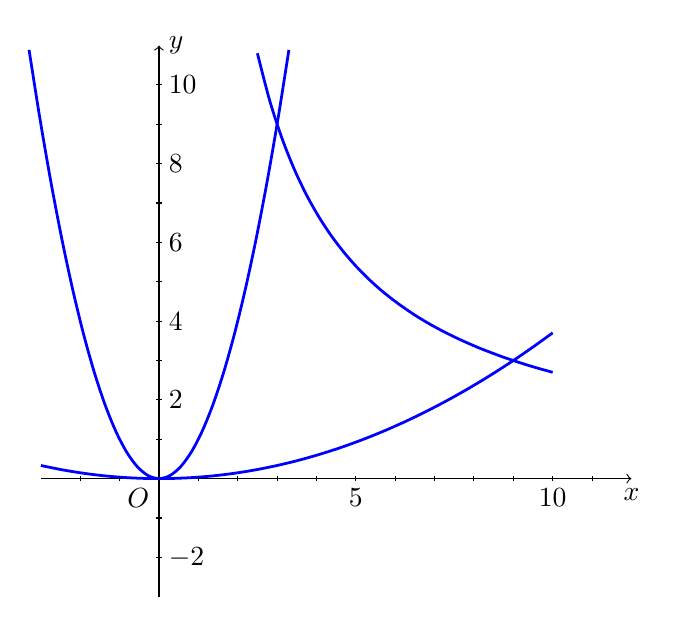
\begin{tikzpicture}[scale=.5]%VD1
			\draw[->] (-3,0)--(12,0);
			\draw[->] (0,-3)--(0,11);
			\draw  (0,0) node[below left]{$O$}  (12,0) node[below]{$x$}  (0,11) node[right]{$y$}   ;
			\draw[smooth,blue,line width=1]
			plot[domain=-3.3:3.3]
			(\x,{(\x)^(2)});
			\draw[smooth,blue,line width=1]
			plot[domain=-3:10]
			(\x,{1/(27)*(\x)^(2)});
			\draw[smooth,blue,line width=1]
			plot[domain=2.5:10]
			(\x,{27*(\x)^-1});
			%f(x) = -0.5x³ + 1.5x
			\foreach \y in {-2,-1,1,2,3,4,5,6,7,8,9,10}
			\draw[shift={(0,\y)}] (2pt,0)--(-2pt,0);
			\foreach \x in {-2,-1,1,2,3,4,5,6,7,8,9,10,11}
			\draw[shift={(\x,0)}] (0,2pt)--(0,-2pt);
			\draw  (5,0) node[below]{$5$} (10,0) node[below]{$10$}
			(0,-2) node[right]{$-2$} (0,2) node[right]{$2$} (0,4) node[right]{$4$} (0,6) node[right]{$6$}
			(0,8) node[right]{$8$} (0,10) node[right]{$10$}
			; 
			\end{tikzpicture}
		\end{center}
		Gọi $(P_1)\colon y=x^2, (P_2)\colon y=\dfrac{x^2}{27}, (H)\colon y=\dfrac{27}{x}$.\\
		Ta đi tìm giao điểm của các đường.\\
		$\begin{aligned}&(P_1)\cap (P_2)\colon x^2=\dfrac{x^2}{27}\Leftrightarrow x=0\Rightarrow y=0\Rightarrow O(0;0)\\&(P_1)\cap (H)\colon x^2=\dfrac{27}{x}\Leftrightarrow x=3\Rightarrow y=9\Rightarrow A(3;9)\\&(P_2)\cap (H)\colon\dfrac{x^2}{27}=\dfrac{27}{x}\Leftrightarrow x=9\Rightarrow y=3\Rightarrow B(9;3)\end{aligned}$.\\
		Diện tích miền S là\\
		\[S=\displaystyle\int\limits_0^3\left(x^2-\dfrac{x^2}{27}\right)\mathrm{\,d}x+\displaystyle\int\limits_3^9\left(\dfrac{27}{x}-x^2\right)\mathrm{\,d}x=27\ln 3-234\]	}
\end{vd}
\begin{vd}%Ví dụ 2:[Trần Lê Vĩnh Phúc]%[2D3K3-1] 
	Diện tích hình phẳng giới hạn bởi các đường: $y=\sqrt{8-x^2};y=\sqrt{2-x^2};y=|x|$ 
	\choice
	{\True $\dfrac{3}{2}\pi$}
	{$3\pi$}
	{$\pi$}
	{$6\pi$}
	\loigiai{
		\begin{center}
			\begin{tikzpicture}[samples=200]%VÍ DỤ 2
			\draw[->] (-4,0)--(4,0);
			\draw[->] (0,-2.3)--(0,4);
			\draw  (0,0) node[below left]{$O$}  (4,0) node[below]{$x$}  (0,4) node[right]{$y$}   ;
			\draw[color=blue] (-2.828427125,0) arc (180:0:2.828427125 cm and 2.828427125 cm);
			\draw[color=blue] (-1.414213562,0) arc (180:0:1.414213562 cm and 1.414213562 cm);	
			\draw[smooth,blue,line width=1]
			plot[domain=-3:3]
			(\x,{abs(\x) });
			%f(x) = -0.5x³ + 1.5x
			\foreach \y in {-2,-1,1,2,3}
			\draw[shift={(0,\y)}] (2pt,0)--(-2pt,0);
			\foreach \x in {-3,-2,-1,1,2,3}
			\draw[shift={(\x,0)}] (0,2pt)--(0,-2pt);
			
			\end{tikzpicture}
		\end{center}
		$(C_1)\colon y=\sqrt{8-x^2};(C_2)y=\sqrt{2-x^2};(d)y=|x|$.\\
		Tìm giao điểm giữa các đường:\\
		$(C_1)\cap(d)\colon\sqrt{8-x^2}=|x|\Leftrightarrow\hoac{&x=2\Rightarrow y=2\Rightarrow A(2;2)\\&x=-2\Rightarrow y=-2\Rightarrow B(-2;2).}$ \\
		$(C_2)\cap(d)\colon\sqrt{2-x^2}=|x|\Leftrightarrow\hoac{&x=1\Rightarrow y=1\Rightarrow C(1;1)\\&x=-1\Rightarrow y=1\Rightarrow D(-1;1).}$ \\
		Diện tích miền S là\\
		$S=\displaystyle\int\limits_{-2}^{-1}\left(\sqrt{8-x^2}+x\right)\mathrm{\,d}x+\displaystyle\int\limits_{-1}^1\left(\sqrt{8-x^2}-\sqrt{2-x^2}\right)\mathrm{\,d}x+\displaystyle\int\limits_1^2\left(\sqrt{8-x^2}-x\right)\mathrm{\,d}x=\dfrac{3}{2}\pi$.\\
		Cách 2: Nếu vẽ phác hình ra nhìn thấy diện tích hình vành khăn là\\
		$S=\dfrac{1}{4}\left(\pi R_1^2-\pi R_2^2\right)=\dfrac{3}{2}\pi$.}
\end{vd}
\begin{vd}%Ví dụ 3.[Trần Lê Vĩnh Phúc]%[2D3G3-1]
	Gọi (H) là hình phẳng giới hạn bởi đồ thị (P) của hàm số $y=6x-x^2$ và trục hoành. Hai đường thẳng $y=m,y=n$ chia hình (H) thành ba phần có diện tích bằng nhau. Tính $P=(9-m)^3+(9-n)^3$ 
	\begin{center}
		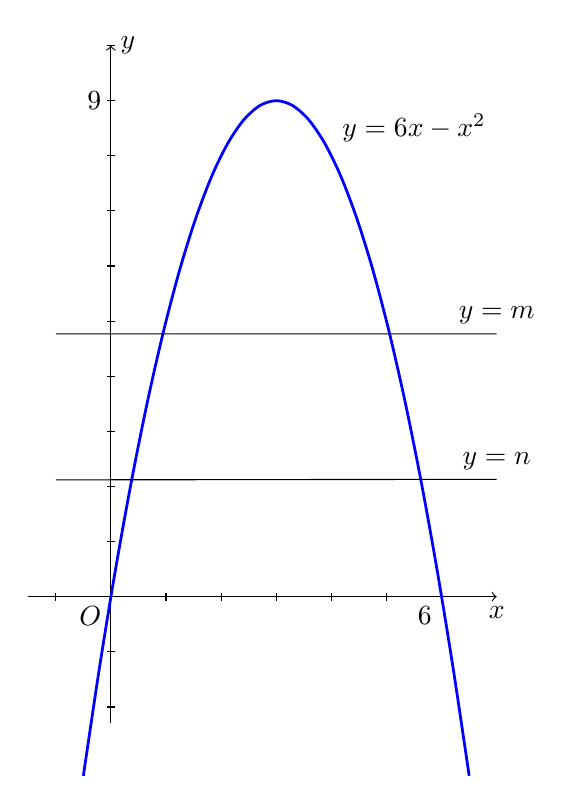
\begin{tikzpicture}[scale=.7]%VÍ DỤ 3
		\draw[->] (-1.5,0)--(7,0);
		\draw[->] (0,-2.3)--(0,10);
		\draw  (0,0) node[below left]{$O$}  (7,0) node[below]{$x$}  (0,10) node[right]{$y$}   ;
		\draw[smooth,blue,line width=1]
		plot[domain=-0.5:6.5]
		(\x,{6*(\x)-(\x)^2 });
		\foreach \y in {-2,-1,1,2,3,4,5,6,7,8,9,10}
		\draw[shift={(0,\y)}] (2pt,0)--(-2pt,0);
		\foreach \x in {-1,1,2,3,4,5,6}
		\draw[shift={(\x,0)}] (0,2pt)--(0,-2pt);
		\draw (0,9) node[left]{$9$}   (6,0)node[below left]{$6$}  (5.5,8.5)node{$y=6x-x^2$};
		\draw (-1,2.12)--(7,2.13)node[above]{$y=n$} (-1,4.77)--(7,4.77)node[above]{$y=m$} ;
		\end{tikzpicture}
	\end{center}
	\choice
	{\True $P=405$}
	{$P=409$}
	{$P=407$}
	{$P=403$}
	\loigiai{
		\textbf{Cách 1: (Dùng công thức diện tích theo biến $y$)}.\\
		\begin{center}
			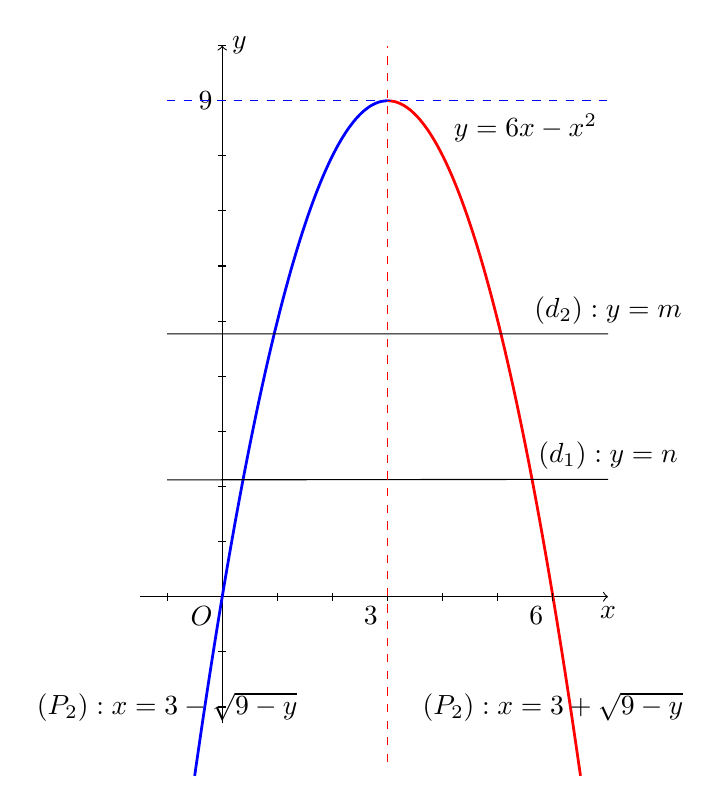
\begin{tikzpicture}[scale=.7]% LỜI GIẢI VÍ DỤ 3
			\draw[->] (-1.5,0)--(7,0);
			\draw[->] (0,-2.3)--(0,10);
			\draw  (0,0) node[below left]{$O$}  (7,0) node[below]{$x$}  (0,10) node[right]{$y$}   ;
			\draw[smooth,blue,line width=1]
			plot[domain=-0.5:3]
			(\x,{6*(\x)-(\x)^2 });
			\draw[smooth,red,line width=1]
			plot[domain=3:6.5]
			(\x,{6*(\x)-(\x)^2 });
			\foreach \y in {-2,-1,1,2,3,4,5,6,7,8,9,10}
			\draw[shift={(0,\y)}] (2pt,0)--(-2pt,0);
			\foreach \x in {-1,1,2,3,4,5,6}
			\draw[shift={(\x,0)}] (0,2pt)--(0,-2pt);
			\draw (0,9) node[left]{$9$}   (6,0)node[below left]{$6$}  (5.5,8.5)node{$y=6x-x^2$} (3,0)node[below left]{$3$};
			\draw (-1,2.12)--(7,2.13)node[above]{$(d_1):y=n$} (-1,4.77)--(7,4.77)node[above]{$(d_2):y=m$} ;
			\draw[dashed,red] (3,-3)--(3,10) (-1,9)--(7,9);
			\draw[dashed,blue] (-1,9)--(7,9);
			\draw (-1,-2)node{$(P_2): x=3-\sqrt{9-y}$} (6,-2)node{$(P_2): x=3+\sqrt{9-y}$};
			\end{tikzpicture}
		\end{center}
		+ Gọi $(H)\colon\heva{&(P)\colon y=6x-x^2\\&Ox\colon y=0\\&x=0, x=6}$. Suy ra: $S=S_H=\displaystyle\int\limits_0^6\left(6x-x^2\right)\mathrm{\,d}x=36$.\\
		Ta có: $y=6x-x^2\Leftrightarrow(x-3)^2=9-y\Leftrightarrow\hoac{&x=3+\sqrt{9-y}\quad(P_1)\\&x=3-\sqrt{9-y}\quad(P_2).}$ \\
		+ Gọi $(H_1)\colon\heva{&(P_1)\colon x=3+\sqrt{9-y}\\&(P_2)\colon x=3-\sqrt{9-y}\\&y=n, y=9.}$ \\
		Suy ra: $S_1=S_{H_1}=\displaystyle\int\limits_n^9\left(3+\sqrt{9-y}-3+\sqrt{9-y}\right)dy=2\displaystyle\int\limits_n^9\sqrt{9-y}dy=\dfrac{4}{3}(\sqrt{9-n})^3$.\\
		Mà $S_1=\dfrac{S}{3}=12$ nên $\dfrac{4}{3}(\sqrt{9-n})^3=12\Leftrightarrow(9-n)^3=81$.\\
		+ Gọi $(H_2)\colon\heva{&(P_1)\colon x=3+\sqrt{9-y}\\&(P_2)\colon x=3-+\sqrt{9-y}\\&y=m, y=9.}$ \\
		Suy ra: $S_2=S_{H_2}=2\displaystyle\int\limits_m^9\sqrt{9-y}dy=\dfrac{4}{3}(\sqrt{9-m})^3$.\\
		Mà $S_2=\dfrac{2S}{3}=24$ nên $\dfrac{4}{3}(\sqrt{9-n})^3=24\Leftrightarrow(9-n)^3=324$.\\
		Vậy $P=81+324=405$.\\
		\textbf{	Cách 2: (Dùng công thức diện tích theo biến $x$)}.\\
		Từ điều kiện bài toán ta có: $0<m,n<9$.\\
		Xét các phương trình hoành độ giao điểm: $6x-x^2=0$.\\
		$6x-x^2=m\Leftrightarrow\hoac{&x=3-\sqrt{9-m}\\&x=3+\sqrt{9-m}}$ và $6x-x^2=n\Leftrightarrow\hoac{&x=3-\sqrt{9-n}\\&x=3+\sqrt{9-n}.}$ \\
		Gọi $D\heva{&y=6x-x^2\\&Ox\\&x=0;x=6}$; $D_M\heva{&y=6x-x^2\\&y=m\\&x=3-\sqrt{9-m};x=3+\sqrt{9+m}}$; $D_N\heva{&y=6x-x^2\\&y=n\\&x=3-\sqrt{9-n};x=3+\sqrt{9+n}.}$ \\
		Khi đó ta có: 
		$S_{D}=\displaystyle\int\limits_{0}^{6}\left(6x-x^2-m\right)\mathrm{\,d}x=36$.\\
		$S_{D_M}=\displaystyle\int\limits_{3-\sqrt{9-m}}^{3+\sqrt{9-m}}\left(6x-x^2-m\right)\mathrm{\,d}x$  $=\left((9-m)x-\dfrac{(x-3)^3}{3}\right)\bigg|_{3-\sqrt{9-m}}^{3+\sqrt{9-m}} =\dfrac{4}{3}\cdot (\sqrt{9-m})^3$.\\
		Chứng minh tương tự ta có: $S_{D_N}=\dfrac{4}{3}\cdot (\sqrt{9-n})^3$.\\
		Theo bài ra ta có: $S_{D_M}=\dfrac{2}{3}\cdot 36=24$ và $S_{D_N}=\dfrac{1}{3}\cdot 36=12$.\\
		Do đó $(9-m)^3=324$ và $(9-n)^3=81$.\\
		Vậy $P=324+81=405$.}
\end{vd}
\subsubsection{Câu hỏi trắc nghiệm}
\begin{ex}%Câu 85.[Trần Lê Vĩnh Phúc]%[2D3B3-1]
	Diện tích hình phẳng giới hạn bởi các đường: $y=x^2,y=\dfrac{x^2}{4},y=\dfrac{2}{x},y=\dfrac{8}{x}$ 
	\choice
	{\True $\dfrac{10}{3}\ln 4$}
	{$\dfrac{10}{3}\ln 2$}
	{$10\ln 4$}
	{$10\ln 2$}
\end{ex}
\begin{ex}%Câu 86.[Trần Lê Vĩnh Phúc]%[2D3K3-1]
	Tính diện tích của những hình phẳng được giới hạn bởi các đường cong \[y=x^3;\ y=x,\ y=2x\] .
	\choice
	{$\dfrac{7}{3}$}
	{$\dfrac{5}{4}$}
	{\True $\dfrac{3}{2}$}
	{$\dfrac{1}{2}$}
\end{ex}
\begin{ex}%Câu 87.[Trần Lê Vĩnh Phúc]%[2D3K3-1]
	Tính diện tích hình phẳng giới hạn bởi các đường:$y=\left|x^2-4x+3\right|$ và $y=x+3$.
	\choice
	{\True $\dfrac{109}{6}$}
	{$\dfrac{103}{3}$}
	{$\dfrac{79}{34}$}
	{$\dfrac{13}{3}$}
\end{ex}
\Closesolutionfile{ans}
% \DAPAN
\inputansbox{10}{ans/ansCD2D3-3.1.4}
\Opensolutionfile{ans}[ans/ansCD2D3-3.1.5]
\begin{dang}{Ứng dụng tích phân tính diện tích hình phẳng giải quyết bài toán về đồ thị hàm số.}
\end{dang}
\subsubsection{Các ví dụ}
\begin{vd}%[Trần Lê Vĩnh Phúc] %[2D3B3-1]
	Cho hàm số $y=f(x)$ có đồ thị trên đoạn $[-1;4]$như hình vẽ dưới. Tính tích phân $\displaystyle\int\limits_{-1}^{4}\left(x\right)\mathrm{\,d}x$. 
	\begin{center}
		\begin{tikzpicture}[scale=1.2]%  VÍ DỤ 1 phần 5
		\draw[->] (-2,0)--(5,0);
		\draw[->] (0,-2)--(0,3.5);
		\draw  (0,0) node[below left]{$O$}  (5,0) node[below]{$x$}  (0,3.5) node[right]{$y$}   ;
		
		\foreach \y in {-1,1,2,3}
		\draw[shift={(0,\y)}] (2pt,0)--(-2pt,0);
		\foreach \x in {-1,1,2,3,4}
		\draw[shift={(\x,0)}] (0,2pt)--(0,-2pt);
		\draw (-1,0) node[below]{$-1$}  (1,0) node[below]{$1$} (2,0) node[below]{$2$} (3,0) node[above]{$3$} (4,0) node[above]{$4$} (0,-1) node[left]{$-1$} (0,2) node[left]{$2$};
		\draw[smooth,line width=1] (-1,0)--(0,2)--(1,2)--(2,0)--(3,-1)--(4,-1) ;
		\draw[dashed,blue,line width=.8] (1,0)--(1,2) (3,0)|-(0,-1) (4,0)|-(0,-1);
		\draw (2,1.5)node{$y=f(x)$};
		\end{tikzpicture}
	\end{center}
	\choice
	{\True $I=\dfrac{5}{2}$}
	{$I=\dfrac{11}{2}$}
	{$I=5$}
	{$I=3$}
	\loigiai{
		Gọi $A(-1;0)$, $B(0;2)$, $C(1; 2)$, $D(2; 0)$,\\
		$E(3;-1)$, $F(4;-1)$, $H(1; 0)$, $K(3; 0)$, $L(4; 0)$.\\
		Khi đó $I=\displaystyle\int\limits_{-1}^4 f(x)\mathrm{\,d}x=\displaystyle\int\limits_{-1}^{\circ} f(x)\mathrm{\,d}x+\displaystyle\int\limits_0^1 f(x)\mathrm{\,d}x+\displaystyle\int\limits_1^2 f(x)\mathrm{\,d}x+\displaystyle\int\limits_2^3 f(x)\mathrm{\,d}x+\displaystyle\int\limits_3^4 f(x)\mathrm{\,d}x$.\\
		$=\displaystyle\int\limits_{-1}^{\circ}|f(x)|\mathrm{\,d}x+\displaystyle\int\limits_0^1|f(x)|\mathrm{\,d}x+\displaystyle\int\limits_1^2|f(x)|\mathrm{\,d}x-\displaystyle\int\limits_2^3|f(x)|\mathrm{\,d}x-\displaystyle\int\limits_3^4|f(x)|\mathrm{\,d}x$.\\
		(do $f(x)\geq 0$, $\forall x\in[-1;2]$ và $f(x)\leq 0$, $\forall x\in[2;4]$).\\
		$=S_{ABO}+S_{OBCH}+S_{HCD}-S_{DKE}-S_{EFLK}$ = $\dfrac{1}{2}2\cdot 1+2\cdot 1+\dfrac{1}{2}\cdot 2\cdot 1-\dfrac{1}{2}1\cdot 1-1\cdot 1=\dfrac{5}{2}$.}
\end{vd}
\begin{vd}%Ví dụ 2.%[Trần Lê Vĩnh Phúc] %[2D3K3-1]
	Gọi $(H)$ là hình phẳng giới hạn bởi đồ thị hàm số $y=x^2-4x+4$, trục tung và trục hoành. Xác định $k$ để đường thẳng $(d)$ đi qua điểm $A(0,4)$ có hệ số góc $k$ chia $(H)\colon$ thành hai phần có diện tích bằng nhau. 
	\choice
	{$k=-4$}
	{$k=-8$}
	{\True $k=-6$}
	{$k=-2$}
	\loigiai{
		\begin{center}
			\begin{tikzpicture}[line join=round, line cap=round,>=stealth,thick,scale=.7]
			\def\hesoa{1}
			\def\hesob{-4}
			\def\hesoc{4}
			\def\xmin{-1}
			\def\xmax{5}
			\def\ymin{-1}
			\def\ymax{5}
			\tikzset{label style/.style={font=\footnotesize}}
			\draw[->] (\xmin,0)--(\xmax,0) node[below left] {$x$};
			\draw[->] (0,\ymin)--(0,\ymax) node[below right] {$y$};
			\draw (0,0) node [below left] {$O$};
			\begin{scope}
			\clip (\xmin,\ymin) rectangle (\xmax,\ymax);
			\draw[samples=200,domain=\xmin:\xmax,smooth,variable=\x] plot (\x,{\hesoa*(\x)^2+\hesob*(\x)+\hesoc});
			\draw[samples=200,domain=\xmin:\xmax,smooth,variable=\x] plot (\x,{-4*(\x)+4});
			\draw[pattern = north east lines, line width = 1.2pt,draw=none](0,0) plot[domain=0:1] (\x, {-4*(\x)+4})--(1,0)--(0,0)--cycle;
			\draw[pattern = north west lines, line width = 1.2pt,draw=none]plot[domain=0:2] (\x, {(\x)^2-4*(\x)+4})--(2,0)--(1,0)--plot[domain=0:1] (\x, {-4*(\x)+4});
			\tkzDrawPoint[fill=black,size=4pt](1,0);
			\tkzDrawPoint[fill=black,size=4pt](2,0);
			\tkzLabelPoint[below left](1,0){$B$};
			\tkzLabelPoint[below](2,0){$I$};		
			\tkzLabelPoint[left](0,4){$4$};	
			\end{scope}
			\tkzLabelPoint[right](1.25,-1.02){$d$};
			\end{tikzpicture}
		\end{center}
		Phương trình hoành độ giao điểm của đồ thị hàm số $y=x^2-4x+4$ và trục hoành là  \[x^2-4x+4=0 \Leftrightarrow x=2\] .\\
		Diện tích hình phẳng  $(H)\colon$ giới hạn bởi đồ thị hàm số: $y=x^2-4x+4$, trục tung và trục hoành là 
		\[S=\displaystyle\int\limits_{0}^{2} \left|x^2-4x+4\right| \mathrm{\,d}x=\displaystyle\int\limits_{0}^{2} \left(x^2-4x+4\right) \mathrm{\,d}x=\left(\dfrac{x^3}{3}-2x^2+4x\right)\bigg|_{0}^{2}=\dfrac{8}{3}  \]
		Phương trình đường thẳng $(d)$ đi qua điểm $A(0;4)$
		có hệ số góc $k$ có dạng: $y=kx+4$.\\
		Gọi $B$ là giao điểm của $(d)$ và trục hoành. \\
		Khi đó $B=\left(\dfrac{-4}{k};0\right)$.\\
		Đường thẳng $(d)$ chia $(H) \colon$ thành hai phần có diện tích bằng nhau khi $B \in OI$ và \\ $S_{\Delta OAB}=\dfrac{1}{2}S=\dfrac{4}{3} \Leftrightarrow \heva{&0<\dfrac{-4}{k}<2 \\&S_{\Delta OAB}=\dfrac{1}{2}OA.OB=\dfrac{1}{2}.4.\dfrac{-4}{k}=\dfrac{-8}{k}}\Leftrightarrow \heva{&k<-2\\&k=-6} \Leftrightarrow k=-6$. 
	}
\end{vd}
\begin{vd}%Ví dụ 3.%[Trần Lê Vĩnh Phúc] %[2D3K3-2]
	Một khuôn viên dạng nửa hình tròn có đường kính bằng $4\sqrt{5}$ (m). Trên đó người thiết kế hai phần để trồng hoa có dạng của một cánh hoa hình parabol có đỉnh trùng với tâm nửa hình tròn và hai đầu mút của cánh hoa nằm trên nửa đường tròn (phần tô màu), cách nhau một khoảng bằng $4$ (m), phần còn lại của khuôn viên (phần không tô màu) dành để trồng cỏ Nhật Bản.\\
	Biết các kích thước cho như hình vẽ và kinh phí để trồng cỏ Nhật Bản là $100\cdot 000$ đồng/m2. Hỏi cần bao nhiêu tiền để trồng cỏ Nhật Bản trên phần đất đó? (Số tiền được làm tròn đến hàng nghìn)
	\begin{center}
		\begin{tikzpicture}[samples=200]%VÍ DỤ 3 PHẦN 5
		\draw[line width=1] (-4.4721,0)--(4.4721,0);
		\fill[red] 
		(0,0) circle (2pt) 
		(-4.4721,0) circle (2pt) 
		(4.4721,0) circle (2pt) 
		;	
		\draw[smooth,blue,line width=1]
		plot[domain=-sqrt(20):sqrt(20)]
		(\x,{sqrt(20-(\x)^(2)) });	
		\draw[smooth,blue,line width=1]
		plot[domain=-2:2]
		(\x,{(\x)^2 });
		\draw[dashed,line width=1] (-2,0)|-(0,4) (2,0)|-(0,4) ;
		\draw (-2.3,2) node{$4m$} (2.3,2) node{$4m$} (0,4) node[below]{$4m$} ;
		\draw[pattern = north east lines, line width = 1.2pt,draw=none] plot[domain=-2:2] (\x, {sqrt(20-(\x)^2)})--plot[domain=-2:2] (\x, {(\x)^2});
		\end{tikzpicture}
	\end{center}
	\choice
	{$3.895.000$ (đồng)}
	{\True $1.948.000$ (đồng)}
	{$2.388.000$ (đồng)}
	{$1.194.000$ (đồng)}
	\loigiai{
		\begin{center}
			\begin{tikzpicture}[samples=200]% LỜI GIẢI VÍ DỤ 3 PHẦN 5
			\draw[line width=1] (-4.4721,0)--(4.4721,0);
			\fill[red] 
			(0,0) circle (2pt) 
			(-4.4721,0) circle (2pt) 
			(4.4721,0) circle (2pt) 
			(2,4) circle (2pt) 
			;
			\draw[smooth,blue,line width=1]
			plot[domain=-sqrt(20):sqrt(20)]
			(\x,{sqrt(20-(\x)^(2)) });
			\draw[smooth,blue,line width=1]
			plot[domain=-2:2]
			(\x,{(\x)^2 });
			\draw[dashed,line width=1] (-2,0)|-(0,4) (2,0)|-(0,4) ;
			\draw (-2.3,2) node{$4m$} (2.3,2) node{$4m$} (0,4) node[below]{$4m$} ;
			\draw[->] (-5,0)--(5,0);
			\draw[->] (0,-2)--(0,5);
			\draw  (0,0) node[below left]{$O$}  (5,0) node[below]{$x$}  (0,5) node[right]{$y$} (2,4) node[above right]{$M(2,4)$}   ;
			\draw[pattern = north east lines, line width = 1.2pt,draw=none] plot[domain=-2:2] (\x, {sqrt(20-(\x)^2)})--plot[domain=-2:2] (\x, {(\x)^2});
			\end{tikzpicture}
		\end{center}
		Đặt hệ trục tọa độ như hình vẽ. Khi đó phương trình nửa đường tròn là \[y=\sqrt{R^2-x^2}=\sqrt{(2\sqrt{5})^2-x^2}=\sqrt{20-x^2}\] 
		Phương trình parabol $(P)$ có đỉnh là gốc $O$ sẽ có dạng $y=ax^2$.\\
		Mặt khác $(P)$ qua điểm $M(2;4)$ do đó: $4=a(-2)^2\Rightarrow a=1$.\\
		Phần diện tích của hình phẳng giới hạn bởi $(P)$ và nửa đường tròn. (phần tô màu).\\
		Ta có công thức $S_1=\displaystyle\int\limits_{-2}^2\left(\sqrt{20-x^2}-x^2\right)\mathrm{\,d}x\cong 11,94m^2$.\\
		Vậy phần diện tích trồng cỏ là $S_{\text{trồng cỏ}}=\dfrac{1}{2}S_{\text{hình tròn}}-S_1\approx 19,47592654$.\\
		Vậy số tiền cần có là $S_{\text{trồng cỏ}}\times 100000\approx 1\cdot 948\cdot 000$ (đồng). đồng.}
\end{vd}
\begin{vd}%Ví dụ 4.%[Trần Lê Vĩnh Phúc] %[2D3K3-2]
	Cho hình phẳng $(H)$ giới hạn bởi các đường $y=\left|x^2-1\right|$ và $y=k,0<k<1$. Tìm $k$ để diện tích của hình phẳng $(H)$ gấp hai lần diện tích hình phẳng được kẻ sọc trong hình vẽ bên. 
	\begin{center}
		\begin{tikzpicture}[samples=200]% VÍ DỤ 4 PHẦN 5
		\draw[->] (-5,0)--(5,0);
		\draw[->] (0,-2)--(0,5);
		\draw  (0,0) node[below left]{$O$}  (5,0) node[below]{$x$}  (0,5) node[right]{$y$}   ;	
		\draw[smooth,blue,line width=1]
		plot[domain=-2.3:2.3]
		(\x,{ abs((\x)^2-1) });	
		\draw[smooth,blue,line width=1,dashed]
		plot[domain=-1.5:-1]
		(\x,{1-(\x)^2 });	
		\draw[smooth,blue,line width=1,dashed]
		plot[domain=1:1.5]
		(\x,{1-(\x)^2 });
		\draw (1,0) node[below]{$1$} 
		(0,1) node[above right]{$1$} 
		;
		\draw[line width=1] (-2,.6)--(2,.6) node[above]{$y=k$};
		\draw[pattern = north east lines, line width = 1.2pt,draw=none] plot[domain=-0.63:0.63] (\x, {1-(\x)^2})--plot[domain=-0.63:0.63] (\x, {0.6});	
		\end{tikzpicture}
	\end{center}
	\choice
	{$k=\sqrt[3]{4}$}
	{$k=\sqrt[3]{2}-1$}
	{$k=\dfrac{1}{2}$}
	{\True $k=\sqrt[3]{4}-1$}
	\loigiai{
		\begin{center}
			\begin{tikzpicture}[samples=200,scale=1.2]% LỜI GIẢI VÍ DỤ 4 PHẦN 5
			\draw[->] (-5,0)--(5,0);
			\draw[->] (0,-2)--(0,5);
			\draw  (0,0) node[below left]{$O$}  (5,0) node[below]{$x$}  (0,5) node[right]{$y$}   ;				
			\draw[smooth,blue,line width=1,dashed]
			plot[domain=-1.5:-1]
			(\x,{1-(\x)^2 });				
			\draw[smooth,blue,line width=1,dashed]
			plot[domain=1:1.5]
			(\x,{1-(\x)^2 });
			\draw (1,0) node[below]{$1$} 
			(0,1) node[above right]{$1$} 
			;
			\draw[line width=1] (-2.5,.6)--(2.5,.6) node[above]{$y=k$}
			;
			\draw[name path=ab] (-2.5,.6)--(2.5,.6);
			\draw[name path=gk] plot[domain=-2.3:2.3,smooth,blue,line width=1]
			(\x,{ abs((\x)^2-1) });
			\fill[name intersections={of=ab and gk,total=\t}]
			\foreach \s in {1,...,\t}{(intersection-\s)coordinate(\s) circle (1.5pt)  };			
			\end{tikzpicture}
		\end{center}
		Do đồ thị nhận trục $Oy$ làm trục đối xứng nên yêu cầu bài toán trở thành:\\
		Diện tích hình phẳng giới hạn bởi $y=1-x^2,y=k,x=0$ bằng diện tích hình phẳng giới hạn bởi: \[y=1-x^2,y=x^2-1,y=k,x>0\]
		$\displaystyle\int\limits_0^{\sqrt{1-k}}\left(1-x^2-k\right)\mathrm{\,d}x=\displaystyle\int\limits_{\sqrt{1-k}}^1\left(k-1+x^2\right)\mathrm{\,d}x+\displaystyle\int\limits_1^{\sqrt{1+k}}\left(k-x^2+1\right)\mathrm{\,d}x$.\\
		$\begin{aligned}&\Leftrightarrow(1-k)\sqrt{1-k}-\dfrac{1}{3}(1-k)\sqrt{1-k}\\&=\dfrac{1}{3}-(1-k)-\dfrac{1}{3}(1-k)\sqrt{1-k}+(1-k)\sqrt{1-k}+(1+k)\sqrt{1+k}-\dfrac{1}{3}(1+k)\sqrt{1+k}-(1+k)+\dfrac{1}{3}\end{aligned}$ \\
		$ \Leftrightarrow\dfrac{2}{3}(1+k)\sqrt{1+k}=\dfrac{4}{3}\Leftrightarrow(\sqrt{1+k})^3=2\Leftrightarrow k=\sqrt[3]{4}-1 $.}
\end{vd}
\subsubsection{Câu hỏi trắc nghiệm}
\begin{ex}%Câu 88.%[Trần Lê Vĩnh Phúc] %[2D3K3-1]
	Cho hàm số $y=\dfrac{1}{3}x^3+mx^2-2x-2m-\dfrac{1}{3}$ có đồ thị $(C)$. Tìm $m\in\left(0;\dfrac{5}{6}\right)$ sao cho hình phẳng giới hạn bởi đồ thị $(C)$ và các đường thẳng $x=0,x=2,y=0$ và có diện tích bằng 4. 
	\choice
	{$m=\dfrac{1}{4}$}
	{$m=\dfrac{1}{3}$}
	{\True $m=\dfrac{1}{2}$}
	{$m=1$}
\end{ex}
\begin{ex}%Câu 89.%[Trần Lê Vĩnh Phúc]%[2D3K3-1]
	\immini{
		Cho $y=f(x)=ax^3+bx^2+cx+d,(a,b,c,d\in\mathbb{R},a\neq 0)$ có đồ thị $(C)$. Biết rằng đồ thị $(C)$ tiếp xúc với đường thẳng $y=4$ tại điểm có hoành độ âm và đồ thị của hàm số $y=f’(x)$ cho bởi hình vẽ bên. Tính diện tích $S$ của hình phẳng giới hạn bởi đồ thị $(C)$ và trục hoành.
	\choice
	{$S=9$}
	{\True $S=\dfrac{27}{4}$}
	{$S=\dfrac{21}{4}$}
	{$S=\dfrac{5}{4}$}
	}{
		\begin{tikzpicture}
		\draw[->] (-3,0)--(3,0);
		\draw[->] (0,-4)--(0,2.5);
		\draw  (0,0) node[below left]{$O$}  (3,0) node[below]{$x$}  (0,4) node[right]{$y$}   ;
		\draw[smooth] plot[domain=-1.5:1.5]
		(\x,{3*(\x)^2-3 });
		\draw (1,0) node[below right]{$1$} 
		(-1,0) node[below left]{$1$} 
		(0,-3) node[below left]{$-3$} 
		;
		\end{tikzpicture}
	}
\end{ex}
\begin{ex}%Câu 90.%[Trần Lê Vĩnh Phúc]%[2D3K3-1]
	Cho hàm số $y=x^4-4x^2+m$ có đồ thị là $(C)$. Gọi $S$ là diện tích hình phẳng giới hạn bởi đồ thị $(C)$ với $y<0$ và trục hoành, là diện tích hình phẳng giới hạn bởi đồ thị $(C)$ với $y>0$ và trục hoành. Với giá trị nào của m thì $S=S’$?
	\choice
	{$m=2$}
	{$m=\dfrac{2}{9}$}
	{\True $m=\dfrac{20}{9}$}
	{$m=1$}
\end{ex}
\begin{ex}%Câu 91.%[Trần Lê Vĩnh Phúc %[2D3K3-7]
	Một vật chuyển động trong 3 giờ với vận tốc $v (km/h)$ phụ thuộc vào thời gian $t (h)$ có đồ thị vận tốc như hình bên. Trong khoảng thời gian $1$ giờ kể từ khi bắt đầu chuyển động, đồ thị đó là một phần của đường parabol có đỉnh $I(2;9)$ và trục đối xứng song song với trục tung, khoảng thời gian còn lại đồ thị là một đoạn thẳng song song với trục hoành. Tính quãng đường $s$ mà vật di chuyển được trong $3$ giờ đó (kết quả làm tròn đến hàng phần trăm). 
	\begin{center}
		\begin{tikzpicture}
		\draw[->] (0,0)--(5,0);
		\draw[->] (0,0)--(0,10);
		\draw  (0,0) node[below left]{$O$}  (5,0) node[below]{$t$}  (0,10) node[right]{$v$}   ;
		\draw plot[domain=0:1] (\x,{-1.25*(\x)^2+5*(\x)+4  });
		\draw[blue,line width=1,dashed]
		plot[domain=1:3]
		(\x,{-1.25*(\x)^2+5*(\x)+4 });
		
		\draw[line width=1] (1,7.75)--(3,7.75);
		
		\fill[red] (0,4) circle (2pt)
		(2,9) circle (2pt)
		(1,7.75) circle (2pt)
		(3,7.75) circle (2pt)
		;
		\draw (1,0) node[below ]{$1$} 
		(2,0) node[below ]{$2$} 
		(3,0) node[below ]{$3$} 
		
		(0,4) node[ left]{$4$} 
		(0,9) node[ left]{$9$} 
		(2,9) node[above]{$I$}
		;
		\draw[dashed,line width=1] (1,7.75)--(1,0) (3,7.75)--(3,0) (2,9)--(2,0);
		\end{tikzpicture}
	\end{center}
	\choice
	{$s=15{,}50 (km)$}
	{$s=13{,}83 (km)$}
	{$s=23{,}25 (km)$}
	{\True $s=21{,}58 (km)$}
\end{ex}
\begin{ex}%Câu 92.%[Trần Lê Vĩnh Phúc] %[2D3B3-1]
	Cho hàm số $y=f(x)$ liên tục trên $[0;4]$ có đồ thị trên $[0;4]$ như hình dưới. 
	\begin{center}
		\begin{tikzpicture}[scale=1.2]%  CÂU 92
		\draw[->] (-2,0)--(5,0);
		\draw[->] (0,-2)--(0,3.5);
		\draw  (0,0) node[below left]{$O$}  (5,0) node[below]{$x$}  (0,3.5) node[right]{$y$}   ;
		
		\foreach \y in {-1,1,2,3}
		\draw[shift={(0,\y)}] (2pt,0)--(-2pt,0);
		\foreach \x in {-1,1,2,3,4}
		\draw[shift={(\x,0)}] (0,2pt)--(0,-2pt);
		\draw (-1,0) node[below]{$-1$}  (1,0) node[below]{$1$} (2,0) node[below]{$2$} (3,0) node[above]{$3$} (4,0) node[above]{$4$} (0,-1) node[left]{$-1$} (0,2) node[left]{$2$};
		\draw[smooth,line width=1] (0,2)--(1,2)--(3,-2)--(4,0) ;
		\draw[dashed,blue,line width=.8] (1,0)--(1,2) (3,0)|-(0,-2) ;
		\draw (2,1.5)node{$y=f(x)$};
		\end{tikzpicture}
	\end{center}
	Tính $\displaystyle\int\limits_0^4 f(x)\mathrm{\,d}x$. 
	\choice
	{$1$}
	{\True $5$}
	{$8$}
	{$0$}
\end{ex}
\Closesolutionfile{ans}
% \DAPAN
\inputansbox{10}{ans/ansCD2D3-3.1.5}